% Báo cáo bài tập lớn TA_DSS - biên dịch bằng pdflatex (MiKTeX hoặc Overleaf)
% Bố cục và trang bìa dựa theo mẫu trong latex_mau/
\documentclass[12pt,a4paper]{article}
\usepackage[utf8]{inputenc}
\usepackage[T5]{fontenc}
\usepackage[vietnamese]{babel}
\usepackage{amsmath, amssymb, amsfonts}
\usepackage{graphicx}
\usepackage{geometry}
\usepackage{indentfirst}
\usepackage{float}
\usepackage{placeins}
\usepackage{booktabs, array, multirow, longtable}
\newcolumntype{R}[1]{>{\raggedleft\arraybackslash}p{#1}}
\usepackage{caption, subcaption}
\captionsetup{justification=centering, font=small, labelfont=bf, skip=6pt}
\captionsetup[sub]{justification=centering, font=footnotesize}
\usepackage{enumitem}
\usepackage{xcolor}
\usepackage{tikz}
\usetikzlibrary{calc, positioning, arrows.meta, decorations.pathmorphing, shapes.geometric}
\usepackage{fancyhdr}
\usepackage{hyperref}
\hypersetup{hidelinks}
\addto\captionsvietnamese{\renewcommand{\refname}{Tài liệu tham khảo}\renewcommand{\listfigurename}{Danh sách hình}\renewcommand{\listtablename}{Danh sách bảng}}

\geometry{margin=2.5cm}
\linespread{1.0}
\emergencystretch=3em
% Kiểm soát cắt trang: không để dòng lẻ đầu/cuối đoạn, cho phép trang cuối chương không kín
\raggedbottom
\widowpenalty=10000
\clubpenalty=10000
\predisplaypenalty=10000
\renewcommand{\topfraction}{0.9}
\renewcommand{\bottomfraction}{0.9}
\renewcommand{\textfraction}{0.1}
\renewcommand{\floatpagefraction}{0.8}
\setcounter{topnumber}{3}
\setcounter{bottomnumber}{2}
\setcounter{totalnumber}{5}
\setlength{\parindent}{17pt}
\setlist{itemsep=2pt,topsep=4pt,parsep=0pt}
\setcounter{secnumdepth}{4}
\setcounter{tocdepth}{3}
\graphicspath{{IMAGE/}}

% Header có logo trường, giống mẫu
\setlength{\headheight}{40pt}
\pagestyle{fancy}
\fancyhead{}
\fancyhead[L]{%
  \begin{tabular}{rl}
    
\includegraphics[width=10mm]{logo_hcmut.png} &
    \parbox[b]{14cm}{%
      \textbf{\ttfamily TRƯỜNG ĐẠI HỌC BÁCH KHOA - ĐHQG-HCM}\\[0.3pt]
      \textbf{\ttfamily KHOA KHOA HỌC VÀ KỸ THUẬT MÁY TÍNH}
    }
  \end{tabular}%
}

\begin{document}

% Trang bìa.
% Mã môn và giảng viên lấy theo tai_lieu_mon_hoc/Lecture 0-Overview.pdf
\begin{titlepage}
	% Khung bìa hai nét
	\begin{tikzpicture}[remember picture, overlay]
		\draw[line width=1.5pt]
		($(current page.north west) + (2cm,-2cm)$)
		rectangle
		($(current page.south east) + (-2cm,2cm)$);
		\draw[line width=0.5pt]
		($(current page.north west) + (2.1cm,-2.1cm)$)
		rectangle
		($(current page.south east) + (-2.1cm,2.1cm)$);
	\end{tikzpicture}

	\begin{center}
		\textbf{ĐẠI HỌC QUỐC GIA THÀNH PHỐ HỒ CHÍ MINH} \\
		\textbf{TRƯỜNG ĐẠI HỌC BÁCH KHOA} \\
		\textbf{KHOA KHOA HỌC \& KỸ THUẬT MÁY TÍNH}
	\end{center}

	\vspace{1cm}
	\begin{center}
		
\includegraphics[width=4.2cm]{logo_hcmut.png}
	\end{center}
	\vspace{1cm}

	\begin{center}
		\begin{tabular}{c}
			\textbf{KHO DỮ LIỆU VÀ HỆ HỖ TRỢ QUYẾT ĐỊNH - CO5113} \\
			\\
			\hline
			\\
			{\huge \textbf{\textit{Báo cáo bài tập lớn}}} \\
			\\
			\hline
		\end{tabular}
	\end{center}

	\begin{center}
		\begin{minipage}{0.8\textwidth}
			\centering
			\textbf{XÂY DỰNG KHO DỮ LIỆU VÀ HỆ HỖ TRỢ RA QUYẾT ĐỊNH DỰ ĐOÁN KHÁCH HÀNG RỜI BỎ, ĐỀ XUẤT CHĂM SÓC GIỮ CHÂN KHÁCH HÀNG CHO DOANH NGHIỆP COMPANYX} \\[0.3cm]
			\textit{Customer Churn Prediction and Retention Decision Support System}
		\end{minipage}
	\end{center}

	\vspace{0.5cm}
	\begin{center}
		\begin{tabular}{rl}
			\textbf{GIẢNG VIÊN HƯỚNG DẪN:} & TS. Phan Trọng Nhân \\
			\textbf{NHÓM:}                 & TA\_DSS \\
			\textbf{SINH VIÊN THỰC HIỆN:}  & Lương Thiên Bảo - 2670198 \\
			                               & Phạm Nguyễn Thùy Dương - 2670202 \\
			                               & Phan Thị Hồng Nhung - 2670221 \\
			                               & Hoàng Ngọc Thủy Thương - 2670234 \\
			                               & Nguyễn Thái Ngọc Giao - 2670206
		\end{tabular}
	\end{center}

	\vfill
	\begin{center}
		{\footnotesize TP. HỒ CHÍ MINH, THÁNG 11/2026}
	\end{center}
	\vspace*{0.5cm}
\end{titlepage}


% Trang danh sách thành viên và tỷ lệ đóng góp (yêu cầu ở slide 12, 13 của Lecture 0).
% Cột "Nội dung công việc" và "Tỷ lệ (%)" để trống, nhóm thống nhất rồi điền.
\section*{Danh sách thành viên và phân công công việc}
\addcontentsline{toc}{section}{Danh sách thành viên và phân công công việc}

\begin{table}[H]
\centering\small
\renewcommand{\arraystretch}{1.9}
\begin{tabular}{clc>{\raggedright\arraybackslash}p{5.4cm}c}
\toprule
\textbf{STT} & \textbf{Họ và tên} & \textbf{MSSV} & \textbf{Nội dung công việc} & \textbf{Tỷ lệ (\%)} \\
\midrule
1 & Lương Thiên Bảo & 2670198 & & \\
2 & Phạm Nguyễn Thùy Dương & 2670202 & & \\
3 & Phan Thị Hồng Nhung & 2670221 & & \\
4 & Hoàng Ngọc Thủy Thương & 2670234 & & \\
5 & Nguyễn Thái Ngọc Giao & 2670206 & & \\
\midrule
\multicolumn{4}{l}{\textbf{Tổng}} & \textbf{100} \\
\bottomrule
\end{tabular}
\end{table}

\clearpage
\tableofcontents
\clearpage
\listoffigures
\clearpage
\listoftables

\clearpage
% Gộp Chương 1 và Chương 2 của tab "Chương 1 + 2 (Updated)" trên Google Doc vào 4 mục của mẫu
\section{Tổng quan bài toán}
\subsection{Bối cảnh và đặt vấn đề}
Trong 19.119 khách hàng từng đặt đơn ở CompanyX, 60,93\% chỉ mua đúng một lần rồi không quay lại. Tính trên 18.995 khách có đơn đã giao, con số là 61,21\%. Số còn lại có mua lặp, nhưng trung vị khoảng cách giữa hai lần mua là 138 ngày. Một khách im lặng bốn tháng có thể chỉ đang nghỉ giữa hai lần mua, cũng có thể đã sang mua ở nơi khác, và dữ liệu không nói đó là trường hợp nào.

CompanyX bán xe đạp, linh kiện và trang phục cho khách lẻ qua kênh trực tuyến và đại lý. Khách lẻ không ký hợp đồng nên không có ngày hết hạn để báo trước, họ chỉ mua thưa dần rồi dừng. Doanh thu lại dựa nhiều vào khách cũ quay lại, nên doanh nghiệp cần biết ai sắp rời đi trước khi họ dừng hẳn.

Trả lời câu hỏi đó vướng ở bốn chỗ. Dữ liệu không có nhãn churn, không ai ghi lại khách nào đã bỏ đi. Số liệu tổng hợp tại một thời điểm không cho biết từng khách đang mua tăng, giữ hay giảm. Thông tin khách, đơn hàng và sản phẩm nằm rải ở nhiều bảng, lẫn cả khách cửa hàng, nên phải tổ chức lại mới tính được chỉ số cho đúng nhóm. Biết ai có nguy cơ vẫn chưa đủ, người quản lý còn phải chọn chăm sóc ai và chi bao nhiêu trong một ngân sách có hạn.

Đề tài trả lời bằng ba phần nối nhau. Kho dữ liệu (Data Warehouse) tổ chức lại dữ liệu giao dịch theo từng khách cá nhân. Mô hình khai phá dữ liệu (Data Mining) học trên kho đó để ước lượng xác suất mỗi khách không mua lại trong kỳ tới. Hệ hỗ trợ ra quyết định (Decision Support System, DSS) đổi xác suất ấy thành danh sách khách nên chăm sóc trong ngân sách người quản lý đặt ra.

\subsection{Mục tiêu nghiên cứu}
Người ra quyết định là quản lý Marketing hoặc Sales. Mỗi kỳ, người này đặt ngân sách chăm sóc, chọn hướng giữ chân và duyệt danh sách khách cần liên hệ. Nhân viên phân tích dữ liệu đưa căn cứ cho quyết định đó, nhân viên chăm sóc khách hàng liên hệ khách theo danh sách đã duyệt. Đề tài làm để người quản lý ấy trả lời được bốn câu hỏi:
\begin{enumerate}[label=\arabic*.]
    \item Khách hàng nào có nguy cơ rời bỏ?
    \item Hành vi mua của khách hàng thay đổi thế nào theo thời gian?
    \item Khách hàng nào cần được ưu tiên giữ chân?
    \item Nên xem xét biện pháp chăm sóc nào cho từng nhóm khách hàng?
\end{enumerate}

Ba mục tiêu nối tiếp nhau đi theo bốn câu hỏi đó. Trước hết là kho dữ liệu theo mô hình chiều, dựng từ cơ sở dữ liệu tác nghiệp, làm nền cho mọi phân tích phía sau. Trên kho, mục tiêu thứ hai là mô hình dự đoán khách nào không quay lại. Dữ liệu không có nhãn, nên nhóm tự đặt luật: khách không phát sinh đơn nào trong 90 ngày sau mốc quan sát được gán nhãn có nguy cơ. Mô hình được đo bằng ma trận nhầm lẫn, accuracy, tỷ lệ lỗi, precision, recall, specificity, F1, ROC-AUC và điểm Brier. Mục tiêu thứ ba là DSS ghép nguy cơ với giá trị khách để chọn ai được chăm sóc khi ngân sách có hạn. DSS không được chấm bằng độ chính xác mà bằng giá trị ròng kỳ vọng $Z$ của danh sách nó chọn ra, vì thứ DSS phải làm tốt là quyết định.

\subsection{Giải pháp tổng thể: hướng tiếp cận bài toán churn}
Trong báo cáo này ``khách rời bỏ'' (customer churn) là khách không mua lại trong 90 ngày sau mốc quan sát (mục 4.3). Định nghĩa này hẹp hơn nghĩa thường: khách bị gắn nhãn hôm nay vẫn có thể quay lại trong ba tháng sau đó, và Bảng~\ref{tab:giaithachthuc} cho thấy trung bình 26,2\% trong số họ làm đúng như vậy. Nhóm chấp nhận độ nhiễu này vì khách bán lẻ không báo khi ngừng mua, và từ dữ liệu giao dịch không có cách nào khác để có nhãn.

Hướng giải đi theo năm bước nối nhau (Hình~\ref{fig:huongtiepcan}), mỗi bước là một chương, kết quả của bước trước là đầu vào của bước sau. Ba thành phần ở mục 1.1 nằm trên chuỗi đó: kho dữ liệu lo phần tổ chức, mô hình lo phần chấm điểm, DSS lo phần chọn khách. Bảng~\ref{tab:giaithachthuc} đối chiếu từng thách thức với thành phần giải nó, kết quả thu được và chương trình bày. Một số mô hình và kỹ thuật trong đó nằm ngoài nội dung môn học, tổng hợp ở mục~\ref{sec:bonus}.

\begin{figure}[!htbp]
\centering
% Sơ đồ năm bước giải bài toán churn, vẽ bằng TikZ (thay cho IMAGE/huong_tiep_can.png của python/ve_so_do_huong_tiep_can.py)
\begin{tikzpicture}[
  buoc/.style={draw=black!70, line width=0.8pt, rounded corners=3pt, fill=white, text width=2.62cm, align=center, inner sep=3pt, minimum height=2.8cm},
  mui/.style={-{Stealth[length=2.5mm]}, line width=0.9pt, black!60},
  giai/.style={font=\scriptsize, text=red!55!black, text width=2.75cm, align=center, inner sep=0pt}]
  \newcommand{\mota}[5]{%
    \node[buoc] (b#1) at (#1*3.27cm, 0) {%
      {\footnotesize\bfseries #2}\\[3pt]
      {\scriptsize #3}\\[4pt]
      {\scriptsize\bfseries\color{black!55} #4}};
    \node[giai, below=3pt of b#1.south] {#5};}
  \mota{0}{1. Kho dữ liệu}{Gom dữ liệu bán hàng vào kho hình sao, chụp hành vi từng khách tại 20 mốc}{Chương 3}{Giải: dữ liệu rải rác, thiếu theo dõi theo thời gian}
  \mota{1}{2. Xác định churn}{Khách không đặt đơn trong 90 ngày sau một mốc là có nguy cơ rời bỏ, tính thuộc tính}{Chương 4}{Giải: dữ liệu chưa có nhãn churn}
  \mota{2}{3. Dự đoán}{Chấm điểm rủi ro cho từng khách, thử mô hình theo đúng trình tự thời gian}{Chương 5}{Trả lời: khách nào có nguy cơ rời bỏ}
  \mota{3}{4. Ra quyết định}{Kết hợp rủi ro với giá trị khách, chọn khách trong ngân sách, gợi ý cách chăm sóc}{Chương 6}{Giải: ưu tiên ai, chi bao nhiêu}
  \mota{4}{5. Đánh giá}{So với cách chọn khách đơn giản, nêu rõ chỗ làm được, chỗ chưa làm được}{Chương 7}{Kiểm tra: có tốt hơn cách đơn giản không}
  \foreach \i/\j in {0/1,1/2,2/3,3/4} \draw[mui] (b\i.east) -- (b\j.west);
\end{tikzpicture}

\caption{Năm bước giải bài toán churn và chương trình bày từng bước}
\label{fig:huongtiepcan}
\end{figure}

\begin{table}[!htbp]
\centering
\caption{Bốn thách thức của bài toán churn, thành phần giải và kết quả}
\label{tab:giaithachthuc}
\footnotesize
\renewcommand{\arraystretch}{1.05}
\begin{tabular}{>{\raggedright\arraybackslash}p{2.4cm}>{\raggedright\arraybackslash}p{1.7cm}>{\raggedright\arraybackslash}p{4.3cm}>{\raggedright\arraybackslash}p{3.9cm}>{\raggedright\arraybackslash}p{1.5cm}}
\toprule
Thách thức & Thành phần giải & Cách giải & Kết quả chính & Trình bày ở \\
\midrule
Dữ liệu chưa có nhãn churn & Khai phá dữ liệu & Tự đặt luật nhãn: khách không đặt đơn nào trong 90 ngày sau một mốc thì có nguy cơ rời bỏ, chia tập học và tập thử theo thời gian & 19 mốc có nhãn đầy đủ. Nhãn còn nhiễu: trung bình 26,2\% khách bị gắn nhãn vẫn mua lại trong ngày 90 đến 180 & Chương 4, 5 và 7 \\
Số liệu tại một thời điểm không cho thấy xu hướng & Kho dữ liệu, khai phá dữ liệu & Bảng Snapshot chụp hành vi từng khách tại 20 mốc, rồi chia khách thành năm nhóm hành vi và ba hạng giá trị & 196.985 dòng Snapshot. Khách chỉ mua một đơn giảm từ 100\% xuống 63,2\% tại mốc chấm điểm & Chương 3, 4 và 6 \\
Dữ liệu rải rác, lẫn khách đại lý & Kho dữ liệu & Kho hình sao, quy trình ETL 11 bước, chỉ giữ khách cá nhân, kiểm tra chất lượng sau khi nạp & 18.484 khách cá nhân, 27.382 đơn. 65 phép kiểm tra đều đạt & Chương 3 \\
Biết nguy cơ chưa đủ để chọn ai & Hệ hỗ trợ ra quyết định & Kết hợp xác suất với giá trị khách thành giá trị ròng kỳ vọng $Z$, chọn khách trong ngân sách, thử giả định (what-if), gợi ý kênh chăm sóc theo quy tắc & Kịch bản cơ sở (ngân sách 40.000 USD): 4.000 khách, $Z$ = 292.595 USD. Kết quả này theo tỷ lệ thành công giả định 10\% & Chương 5 và 6 \\
\bottomrule
\end{tabular}
\end{table}

\subsection{Phạm vi nghiên cứu}
\begin{itemize}
    \item \textbf{Đối tượng:} 18.484 khách hàng cá nhân. Mọi đơn của nhóm này đặt trực tuyến (cờ \texttt{OnlineOrderFlag} bằng 1). Khách đại lý bị loại vì họ nhập hàng theo chu kỳ B2B, nhịp mua của họ không nói gì về chuyện người tiêu dùng có quay lại hay không.
    \item \textbf{Dữ liệu:} đơn hàng từ 31/05/2011 đến 30/06/2014. Lịch sử chia thành giai đoạn quan sát và giai đoạn kiểm tra mua lại, nên khi dự đoán mô hình chỉ được nhìn quá khứ.
    \item \textbf{Phân tích:} ba đặc trưng hành vi Recency, Frequency và Monetary (RFM), thêm hai thuộc tính về sản phẩm đã mua là BikeBuyer (đã mua xe đạp hay chưa) và NSub (số nhóm sản phẩm đã mua). Mô hình chấm điểm dùng năm thuộc tính này, các mô hình đối chứng dùng cả 11 thuộc tính của bảng Snapshot (Chương 4). Tất cả tính được từ riêng dữ liệu giao dịch. Cơ sở dữ liệu gốc còn có nhân khẩu học, vùng bán hàng và lý do mua, phiên bản này chưa đưa vào kho, Chương 7 thử riêng phần đó.
    \item \textbf{Công nghệ:} SQL Server và T-SQL cho kho và quy trình ETL, nguồn với kho ở cùng một nền tảng. Python (pandas, scikit-learn) cho mô hình, Streamlit cho giao diện DSS.
    \item \textbf{Ranh giới:} hệ thống xếp hạng khách và đề xuất chia ngân sách, không tự gửi tin nhắn đến khách. Khách có thật sự ở lại hay không chỉ biết được sau khi triển khai, báo cáo này không đo được điều đó.
\end{itemize}

\subsection{Mô tả tập dữ liệu}
Cơ sở dữ liệu tác nghiệp \texttt{CompanyX} có 72 bảng trong 6 schema, đề tài chỉ chạm tới 9 bảng về hành vi mua (Bảng~\ref{tab:bang_nguon}). Đơn hàng trải 37 tháng với 31.465 đơn, 121.317 dòng chi tiết và tổng thanh toán 123,16 triệu USD. Bảng \texttt{Customer} có 19.820 bản ghi, 701 trong số đó chưa từng đặt đơn.

\begin{table}[!htbp]
\centering\footnotesize
\caption{Các bảng nguồn được sử dụng trong đề tài}
\label{tab:bang_nguon}
\begin{tabular}{lr>{\raggedright\arraybackslash}p{7.8cm}}
\toprule
\textbf{Bảng nguồn} & \textbf{Số dòng} & \textbf{Nội dung} \\
\midrule
\texttt{Sales.SalesOrderHeader} & 31.465 & Thông tin chung của đơn hàng: khách hàng, ngày đặt, ngày giao, trạng thái, tổng tiền \\
\texttt{Sales.SalesOrderDetail} & 121.317 & Chi tiết từng sản phẩm trong đơn: số lượng, đơn giá, chiết khấu \\
\texttt{Sales.Customer} & 19.820 & Danh sách khách hàng, phân biệt khách cá nhân và cửa hàng \\
\texttt{Person.Person} & 19.972 & Họ tên của khách hàng cá nhân \\
\texttt{Sales.SalesTerritory} & 10 & Khu vực bán hàng và nhóm quốc gia \\
\texttt{Sales.SpecialOffer} & 16 & Chương trình khuyến mãi áp dụng cho dòng đơn \\
\texttt{Production.Product} & 504 & Danh mục sản phẩm \\
\texttt{Production.ProductSubcategory} & 37 & Tiểu loại sản phẩm \\
\texttt{Production.ProductCategory} & 4 & Loại sản phẩm: Bikes, Components, Clothing, Accessories \\
\bottomrule
\end{tabular}
\end{table}

Hai thứ dữ liệu không có. Không có nhãn churn, nên nhãn phải suy từ luật 90 ngày ở mục 1.2. Không có dữ liệu chăm sóc khách hàng (CRM) hay lịch sử chiến dịch, nên tỷ lệ khách quay lại nhờ được chăm sóc và chi phí mỗi lần liên hệ đều là tham số giả định. Người quản lý chỉnh hai tham số này ngay trên giao diện DSS, và mọi con số giá trị ròng trong báo cáo đều đứng trên giả định đó.

\clearpage
% Nội dung lấy từ slide môn học (ngày 03/11/2026), chỉ giữ các khái niệm mà Chương 3 đến 7 dùng tới
% Hình trong IMAGE/slide/ cắt từ PDF slide ở docs/ bằng script, hình thành phần DSS và 14 đặc trưng vẽ bằng TikZ
\section{Cơ sở lý thuyết}
Mỗi khái niệm trong chương này có mặt vì một chương sau cần tới nó: kho dữ liệu và ETL cho Chương 3, khai phá dữ liệu và cách đo mô hình cho Chương 4 và 5, hệ hỗ trợ ra quyết định cho Chương 6 và 7. Chỗ nào vượt ra ngoài tài liệu môn học thì ghi rõ ngay tại chỗ.

\subsection{Kho dữ liệu}
\subsubsection{Định nghĩa và đặc trưng}
Trong bốn đặc trưng mà Inmon~\cite{inmon2005} gán cho kho dữ liệu, đặc trưng cuối quyết định cách đề tài dựng bảng Snapshot ở Chương 3: kho gắn với thời gian, lưu lịch sử như các ảnh chụp liên tiếp thay vì chỉ giữ trạng thái hiện hành. Ba đặc trưng còn lại là hướng chủ đề (tổ chức theo khách hàng, sản phẩm, doanh số thay vì theo ứng dụng), tích hợp (thống nhất tên và mã hoá từ nhiều nguồn) và không biến động (dữ liệu đã nạp thì chủ yếu để đọc, không sửa liên tục). Bản thân kho dữ liệu (Data Warehouse) là nơi lưu trữ tập trung để phân tích và ra quyết định, gom dữ liệu từ các hệ thống tác nghiệp, làm sạch, chuẩn hoá rồi sắp xếp lại cho phân tích~\cite{inmon2005,kimball2013}.

Hình~\ref{fig:kien_truc_dw} là kiến trúc tổng quát~\cite{elmasri2016}: dữ liệu đi từ các nguồn, qua ETL, vào kho, rồi phục vụ OLAP, DSS và khai phá dữ liệu. Cơ sở dữ liệu tác nghiệp (OLTP) của CompanyX và kho của đề tài khác nhau ở mục đích lẫn cách thiết kế, Bảng~\ref{tab:oltp_olap} đặt hai bên cạnh nhau~\cite{han2011}.

\begin{figure}[!htbp]
\centering
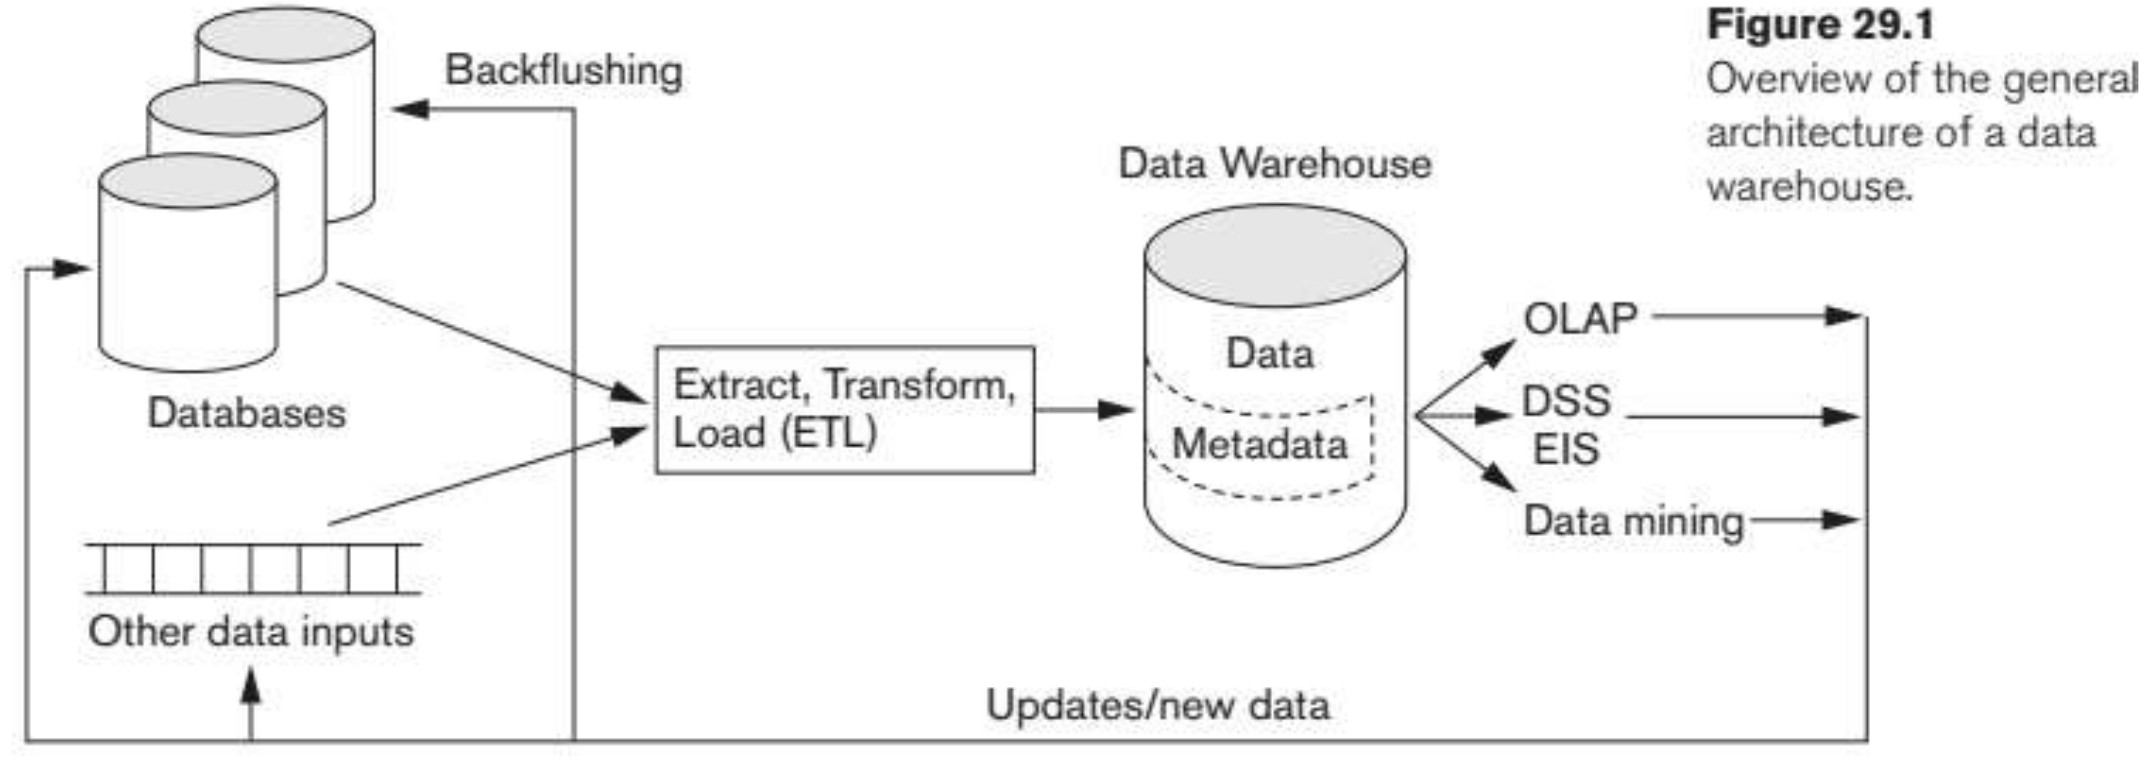
\includegraphics[width=0.9\textwidth]{slide/kien_truc_dw.png}
\caption{Kiến trúc tổng quát của kho dữ liệu}
\label{fig:kien_truc_dw}
\end{figure}

\begin{table}[!htbp]
\centering
\caption{So sánh hệ thống OLTP và OLAP}
\label{tab:oltp_olap}
\begin{tabular}{p{3.2cm}p{5cm}p{5.5cm}}
\toprule
\textbf{Tiêu chí} & \textbf{OLTP} & \textbf{OLAP} \\
\midrule
Định hướng & Giao dịch & Phân tích \\
Người dùng & Nhân viên nhập liệu, quản trị CSDL & Nhà quản lý, chuyên viên phân tích \\
Thiết kế CSDL & Mô hình ER, chuẩn hoá cao & Mô hình sao hoặc bông tuyết, phi chuẩn hoá \\
Dữ liệu & Hiện hành, chi tiết & Lịch sử, tổng hợp, đa chiều \\
Truy cập & Đọc và ghi & Chủ yếu là đọc \\
Đơn vị công việc & Giao dịch ngắn, đơn giản & Truy vấn phức tạp \\
\bottomrule
\end{tabular}
\end{table}

\subsubsection{Mô hình hoá chiều}
Kho ở Chương 3 là một mô hình sao, kiểu thiết kế mà Kimball gọi là mô hình hoá chiều~\cite{kimball2013}. Giữa sao là bảng sự kiện (fact) chứa số đo của nghiệp vụ, ví dụ số tiền bán, cùng khoá ngoại trỏ tới các bảng chiều. Quanh nó là bảng chiều (dimension) chứa thuộc tính mô tả để lọc và nhóm: ngày, sản phẩm, khách hàng. Khi bảng chiều tách nhỏ theo cấp bậc, sao thành bông tuyết (Hình~\ref{fig:sao_bong_tuyet}, vẽ lại theo~\cite{empire}). Kimball thiết kế theo bốn bước: chọn quy trình nghiệp vụ, khai báo độ mịn (một dòng sự kiện thể hiện điều gì), xác định các chiều, xác định các số đo. Thuộc tính của chiều đổi theo thời gian thì xử lý bằng chiều thay đổi chậm (SCD): kiểu 1 ghi đè giá trị cũ, kiểu 2 thêm dòng mới để giữ lịch sử.

\begin{figure}[!htbp]
\centering
% Vẽ lại theo hình trong slide (ảnh cắt từ slide bị chồng hình)
\tikzset{
    chieu/.style={draw, font=\scriptsize, align=center, minimum width=13mm, minimum height=6mm, inner sep=2pt},
    sukien/.style={chieu, fill=gray!15, thick, minimum width=15mm, minimum height=9mm}}
\begin{subfigure}[b]{0.40\textwidth}
    \centering
    \begin{tikzpicture}
        \node[sukien] (fact) {Sales\\Facts};
        \node[chieu, above left=4mm and 3mm of fact] (time) {Time};
        \node[chieu, above right=4mm and 3mm of fact] (cust) {Customer};
        \node[chieu, below left=4mm and 3mm of fact] (prod) {Product};
        \node[chieu, below right=4mm and 3mm of fact] (sell) {Seller};
        \foreach \n in {time,cust,prod,sell} \draw (fact) -- (\n);
    \end{tikzpicture}
    \caption{Mô hình sao}
\end{subfigure}
\hfill
\begin{subfigure}[b]{0.56\textwidth}
    \centering
    \begin{tikzpicture}
        \node[sukien] (fact) {Sales\\Facts};
        \node[chieu, above left=4mm and 3mm of fact] (time) {Time};
        \node[chieu, above right=4mm and 3mm of fact] (cust) {Customer};
        \node[chieu, below left=4mm and 3mm of fact] (prod) {Product};
        \node[chieu, below right=4mm and 3mm of fact] (sell) {Seller};
        \node[chieu, left=3mm of time] (month) {Month};
        \node[chieu, right=3mm of cust] (region) {Region};
        \node[chieu, left=3mm of prod] (cat) {Category};
        \node[chieu, right=3mm of sell] (outlet) {Outlet};
        \foreach \n in {time,cust,prod,sell} \draw (fact) -- (\n);
        \draw (time) -- (month); \draw (cust) -- (region);
        \draw (prod) -- (cat); \draw (sell) -- (outlet);
    \end{tikzpicture}
    \caption{Mô hình bông tuyết}
\end{subfigure}
\caption{Mô hình sao và mô hình bông tuyết}
\label{fig:sao_bong_tuyet}
\end{figure}

\subsubsection{Quy trình ETL và chất lượng dữ liệu}\label{sec:ltetl}
ETL gồm ba bước: trích xuất (Extract) lấy dữ liệu từ nguồn, biến đổi (Transform) làm sạch, đổi định dạng và hợp nhất, nạp (Load) đưa vào kho. Biến thể ELT nạp dữ liệu thô vào kho trước rồi mới biến đổi. Chỗ khó không nằm ở ba động từ đó mà ở tích hợp: các nguồn đặt tên hay mã hoá khác nhau, dữ liệu thiếu, sai hay không nhất quán, nên ETL phải kiểm tra chất lượng trước khi ai đó tin vào kho. Tài liệu môn học~\cite{tlmh} chấm chất lượng dữ liệu theo sáu chiều, và Chương 7 dùng đúng sáu chiều này cho kho của đề tài: tính đầy đủ (tỷ lệ dữ liệu đã lưu so với mức đầy đủ), tính duy nhất (mỗi đối tượng chỉ ghi một lần), tính kịp thời (dữ liệu phản ánh đúng thực tế tại thời điểm cần dùng), tính hợp lệ (đúng định dạng, kiểu và miền giá trị), tính chính xác (mô tả đúng đối tượng trong thực tế) và tính nhất quán (không khác biệt giữa các cách biểu diễn của cùng một đối tượng).

\subsubsection{Phân tích đa chiều (OLAP)}
OLAP xem dữ liệu như một khối nhiều chiều: mỗi chiều là một trục (thời gian, sản phẩm, khu vực), mỗi ô chứa một số đo. Trên khối đó có bốn phép cơ bản~\cite{han2011}: roll-up gộp lên mức tổng quát hơn (từ tháng lên quý), drill-down xuống mức chi tiết hơn, slice cố định một chiều để lấy một lát cắt, dice đặt điều kiện trên nhiều chiều để lấy một khối con (Hình~\ref{fig:olap})~\cite{empire}. Dashboard ở Chương 6 làm bốn phép này bằng truy vấn tổng hợp trên kho, không có máy chủ OLAP riêng.

\begin{figure}[!htbp]
\centering
\begin{subfigure}[b]{0.40\textwidth}
    \centering
    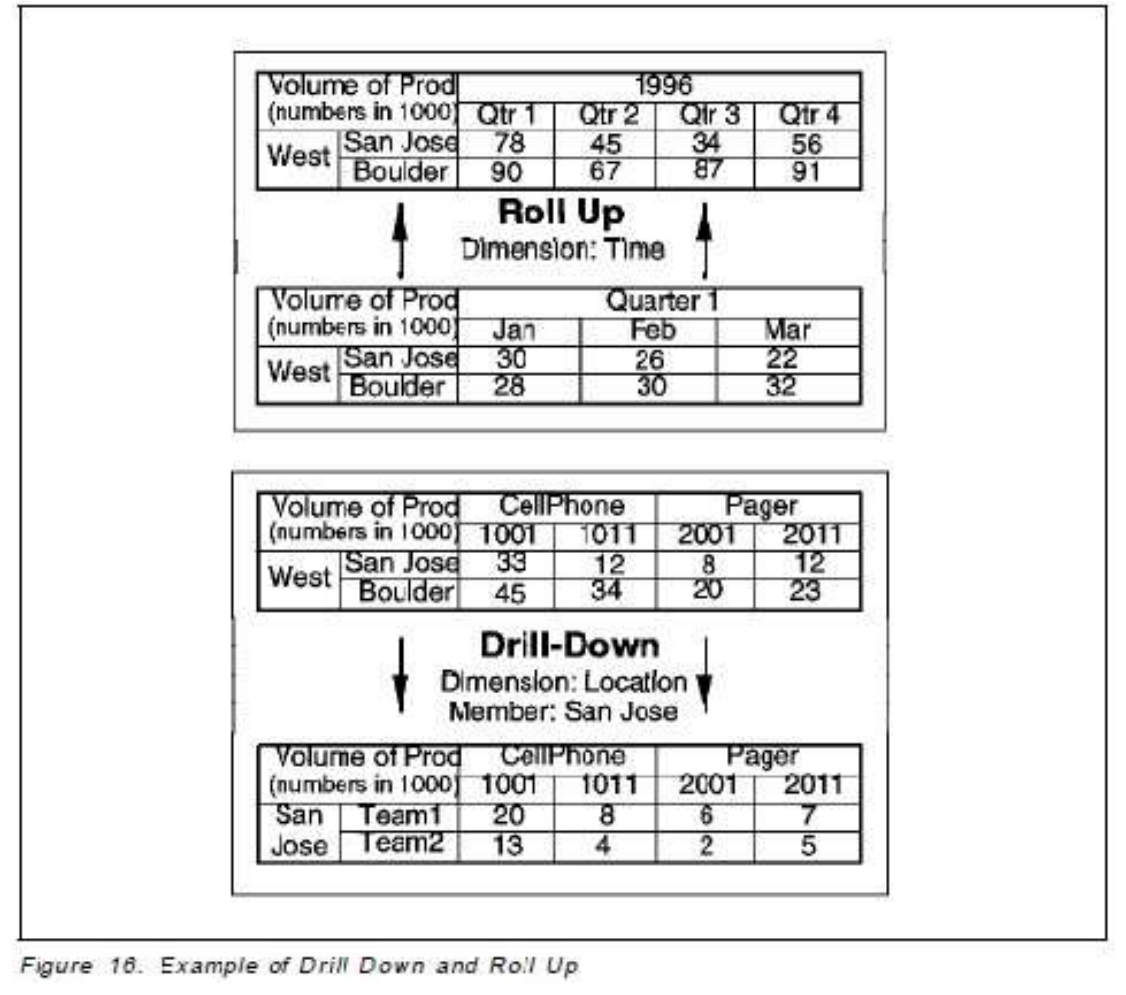
\includegraphics[width=\textwidth]{slide/rollup_drilldown.png}
    \caption{Roll-up và drill-down}
\end{subfigure}
\hfill
\begin{subfigure}[b]{0.56\textwidth}
    \centering
    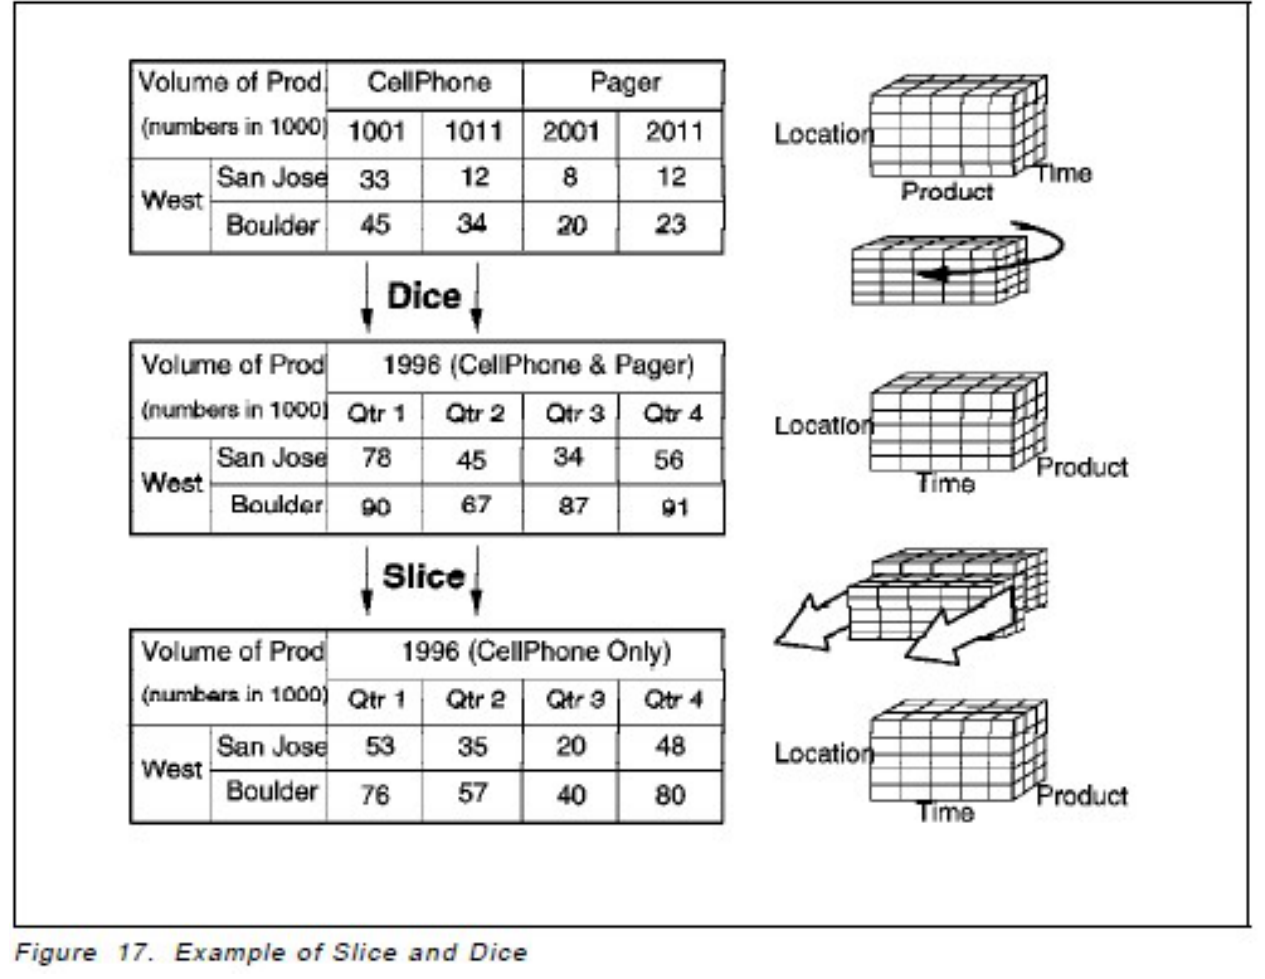
\includegraphics[width=\textwidth]{slide/slice_dice.png}
    \caption{Dice và slice}
\end{subfigure}
\caption{Các phép thao tác OLAP}
\label{fig:olap}
\end{figure}

\subsection{Hệ hỗ trợ ra quyết định}
\subsubsection{Định nghĩa và quá trình ra quyết định}
Bốn pha ra quyết định của Simon (Hình~\ref{fig:simon}) là khung mà Chương 6 dùng để xếp các màn hình của DSS: tìm hiểu (intelligence) phát hiện và phát biểu vấn đề, thiết kế (design) dựng mô hình với các biến và quan hệ giữa chúng, lựa chọn (choice) chọn một giải pháp từ mô hình, thực hiện (implementation) đưa giải pháp vào thực tế. Kết quả thực hiện được theo dõi và phản hồi về các pha trước. Hệ hỗ trợ ra quyết định (DSS), theo Turban và Aronson~\cite{turban2005}, là hệ thống thông tin giúp hỗ trợ và cải thiện việc ra quyết định.

\begin{figure}[!htbp]
\centering
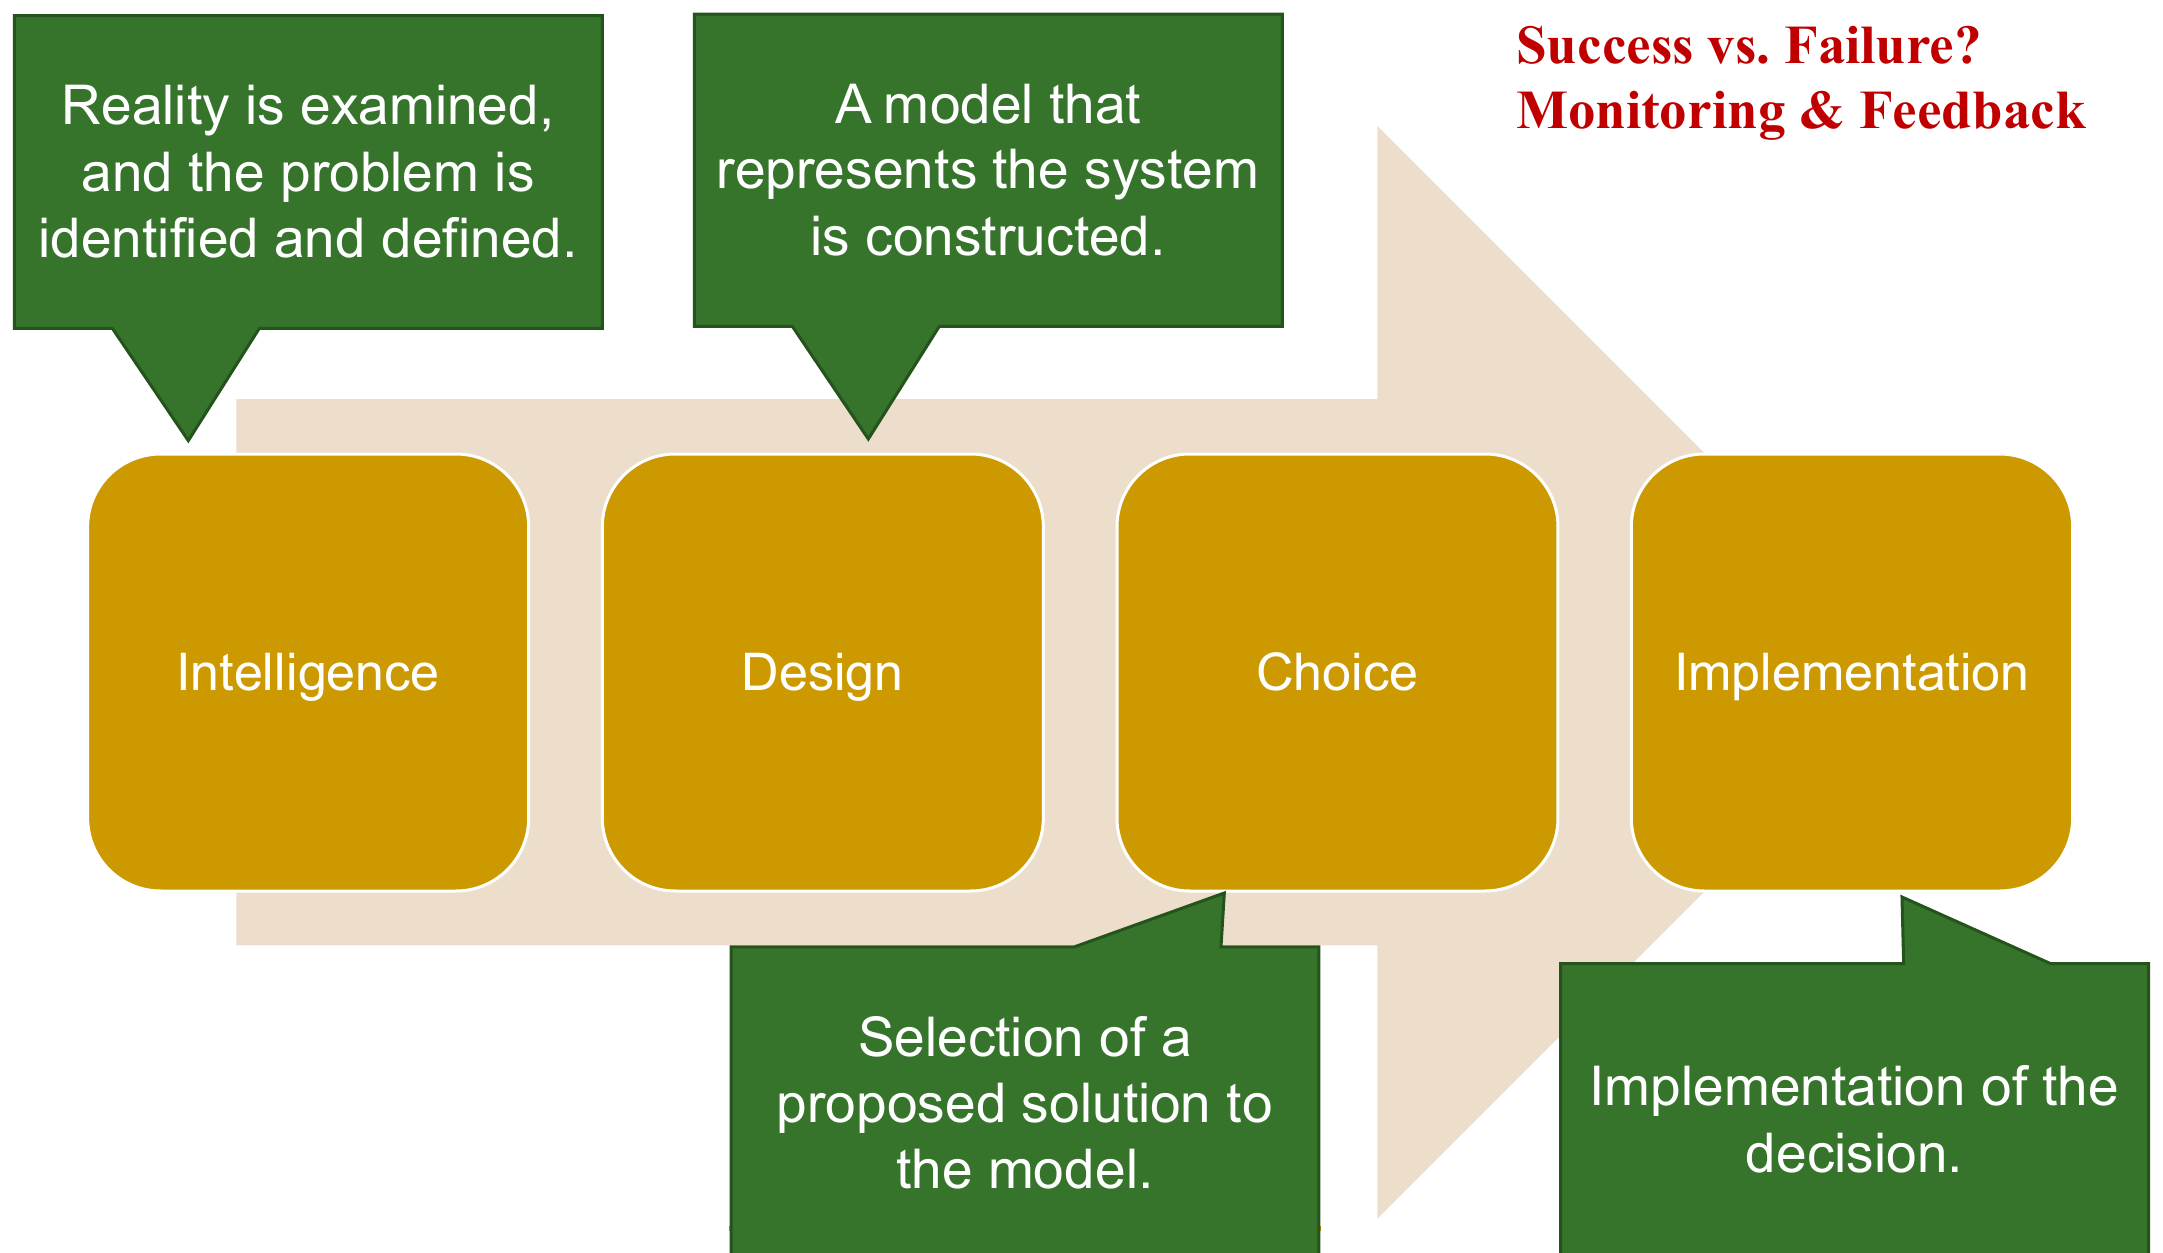
\includegraphics[width=0.72\textwidth]{slide/simon.png}
\caption{Bốn pha của quá trình ra quyết định theo Simon}
\label{fig:simon}
\end{figure}

\subsubsection{Đặc điểm và thành phần của DSS}
DSS hỗ trợ các vấn đề bán cấu trúc và phi cấu trúc cho nhà quản lý ở mọi cấp, nhắm tới hiệu quả của quyết định hơn là hiệu suất tính toán, và con người vẫn kiểm soát máy. Đó là ba trong 14 đặc điểm mà Turban và Aronson~\cite{turban2005} liệt kê (Hình~\ref{fig:dac_trung_dss}). Chương 6 nêu những đặc điểm trong số này mà hệ thống của đề tài đáp ứng đầy đủ.

\begin{figure}[!htbp]
\centering
% Vẽ lại từ hình trong slide (bản scan bị lỗi chữ): DSS ở giữa, bảy đặc điểm mỗi bên
\begin{tikzpicture}[
    dd/.style={draw=black!70, rounded corners=2pt, fill=white, align=left, text width=5.5cm, font=\footnotesize, inner sep=3pt, minimum height=9mm},
    day/.style={black!50, thin}]
    \foreach \i/\chu in {
        1/{(1) Vấn đề bán cấu trúc và phi cấu trúc},
        2/{(2) Hỗ trợ nhà quản lý ở mọi cấp},
        3/{(3) Hỗ trợ cá nhân và nhóm},
        4/{(4) Quyết định phụ thuộc nhau hoặc tuần tự},
        5/{(5) Hỗ trợ đủ bốn pha ra quyết định},
        6/{(6) Nhiều phong cách và quy trình ra quyết định},
        7/{(7) Thích nghi và linh hoạt}} {
        \node[dd, anchor=east] (t\i) at (-1.5, {-(\i-1)*1.0}) {\chu};
    }
    \foreach \i/\chu in {
        8/{(8) Tương tác, dễ sử dụng},
        9/{(9) Hiệu quả, không chỉ hiệu suất},
        10/{(10) Con người kiểm soát máy},
        11/{(11) Người dùng cuối dễ tự phát triển},
        12/{(12) Mô hình hoá và phân tích},
        13/{(13) Truy cập dữ liệu},
        14/{(14) Độc lập, tích hợp hoặc trên nền Web}} {
        \node[dd, anchor=west] (t\i) at (1.5, {-(\i-8)*1.0}) {\chu};
    }
    \node[draw, thick, rounded corners=3pt, fill=gray!15, minimum width=18mm, minimum height=10mm, font=\small\bfseries] (dss) at (0, -3.0) {DSS};
    \foreach \i in {1,...,7} \draw[day] (dss.west) -- (t\i.east);
    \foreach \i in {8,...,14} \draw[day] (dss.east) -- (t\i.west);
\end{tikzpicture}
\caption{Mười bốn đặc điểm của DSS}
\label{fig:dac_trung_dss}
\end{figure}

Bốn thành phần của một DSS (Hình~\ref{fig:thanh_phan_dss})~\cite{turban2005} cũng là bốn phân hệ của hệ thống ở Chương 6: quản lý dữ liệu (lấy dữ liệu từ kho hoặc nguồn khác), quản lý mô hình (lưu và chạy các mô hình thống kê, tài chính, khoa học quản lý), quản lý tri thức (quy tắc nghiệp vụ và tri thức chuyên gia) và giao diện người dùng.

\begin{figure}[!htbp]
\centering
\begin{tikzpicture}[
    tp/.style={draw=black!70, rounded corners=2pt, fill=white, minimum width=30mm, minimum height=10mm, align=center, font=\small},
    noi/.style={{Stealth[length=2mm]}-{Stealth[length=2mm]}, thick}]
    \node[tp] (data) {Quản lý dữ liệu};
    \node[tp, right=14mm of data] (model) {Quản lý mô hình};
    \node[tp, fill=gray!15, thick, below=8mm of $(data)!0.5!(model)$] (ui) {Giao diện người dùng};
    \node[tp, right=10mm of model, yshift=-9mm] (kb) {Quản lý tri thức};
    \node[tp, below=8mm of ui] (user) {Người ra quyết định};
    \draw[noi] (data) -- (model);
    \draw[noi] (data) -- (ui);
    \draw[noi] (model) -- (ui);
    \draw[noi] (kb) -- (ui);
    \draw[noi] (ui) -- (user);
    \node[tp, left=10mm of data] (src) {Kho dữ liệu,\\nguồn khác};
    \draw[-{Stealth[length=2.5mm]}, thick] (src) -- (data);
\end{tikzpicture}
\caption{Các thành phần của một DSS}
\label{fig:thanh_phan_dss}
\end{figure}

\subsubsection{Mô hình hoá và phân tích trong DSS}
Giá trị ròng $Z$ mà Chương 6 cực đại hoá là một biến kết quả theo cách phân loại của Turban và Aronson~\cite{turban2005}. Mô hình toán trong DSS có ba loại biến: biến quyết định là những gì người ra quyết định chọn được, biến không kiểm soát được (tham số) là yếu tố môi trường như giới hạn ngân sách, biến kết quả đo mức độ đạt mục tiêu. Bài toán phối hợp sản phẩm (product-mix) là ví dụ kinh điển: tìm số lượng từng sản phẩm để cực đại $Z$ trong giới hạn tài nguyên, giải bằng quy hoạch tuyến tính hoặc quy hoạch nguyên. Thay sản phẩm bằng khách hàng và tài nguyên bằng ngân sách chăm sóc, ta có bài toán ở Chương 6.

Quyết định diễn ra trong một trong ba điều kiện. Chắc chắn: biết chính xác kết quả của mỗi phương án. Rủi ro: mỗi phương án có nhiều kết quả và biết xác suất của từng kết quả, lúc đó chọn phương án có giá trị kỳ vọng lớn nhất:
\begin{equation}
    EV(a) = \sum_{k} P(s_k)\, v(a, s_k)
\end{equation}
với $P(s_k)$ là xác suất của tình huống $s_k$ và $v(a, s_k)$ là kết quả của phương án $a$ trong tình huống đó. Bất định: không ước lượng được xác suất, nên chọn theo cách lạc quan (maximax) hoặc bi quan (maximin). Chương 5 dùng điều kiện rủi ro với xác suất lấy từ mô hình, còn Chương 6 phải dùng cả ba cách khi tỷ lệ thành công của chăm sóc chưa đo được.

Có mô hình rồi, DSS cho người dùng xoay phương án theo bốn kiểu phân tích~\cite{turban2005}: what-if (đổi một giả định rồi xem kết quả), độ nhạy (đổi một biến nhiều lần để xem kết quả nhạy đến đâu), tìm mục tiêu (tìm đầu vào cần có để đạt một mục tiêu) và tối ưu hoá (tìm giá trị tốt nhất của biến mục tiêu). Chương 6 dùng cả bốn.

\subsection{Phương pháp khai phá dữ liệu}
Đề tài dùng ba bài toán khai phá dữ liệu: phân lớp để chấm điểm nguy cơ, gom cụm để chia nhóm khách, luật kết hợp để gợi ý sản phẩm. Khai phá dữ liệu là quá trình tìm mẫu và tri thức có ích từ dữ liệu lớn~\cite{han2011}, một bước trong quy trình khám phá tri thức (KDD) ở Hình~\ref{fig:kdd}: làm sạch và tích hợp, đưa vào kho, chọn và biến đổi, khai phá, đánh giá và trình bày. Chương 3 và 4 lo các bước trước khai phá, Chương 5 và 6 lo hai bước sau.

\begin{figure}[!htbp]
\centering
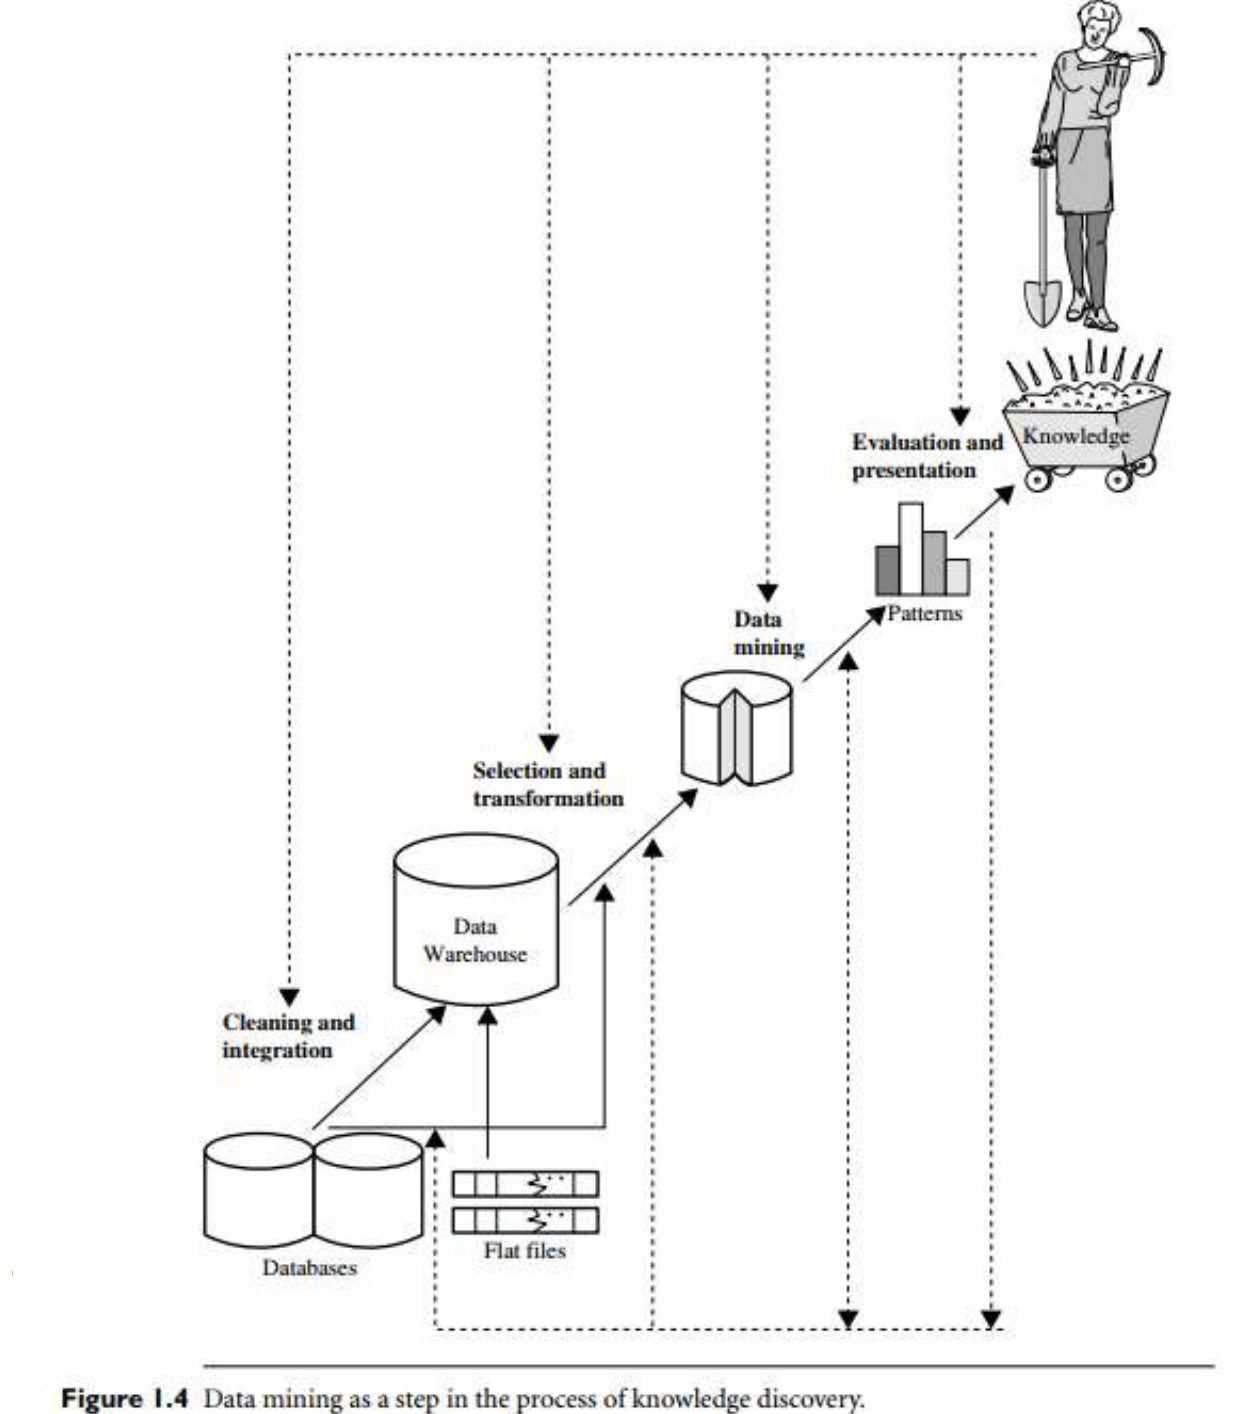
\includegraphics[width=0.4\textwidth]{slide/kdd.png}
\caption{Khai phá dữ liệu là một bước trong quy trình khám phá tri thức}
\label{fig:kdd}
\end{figure}

\subsubsection{Phân lớp và đánh giá mô hình}
Phân lớp (classification) đi qua hai bước~\cite{han2011}: bước học dựng mô hình từ tập huấn luyện đã có nhãn, bước phân lớp dùng mô hình đoán nhãn cho dữ liệu mới. Giữa hai bước, mô hình phải qua một tập thử có nhãn khác tập huấn luyện. Với hai lớp, kết quả thử gói trong ma trận nhầm lẫn (Bảng~\ref{tab:ma_tran_nham_lan}), từ đó ra sáu chỉ số~\cite{han2011}:
\begin{align}
    \text{Accuracy} &= \frac{TP + TN}{P + N}, &
    \text{Error rate} &= \frac{FP + FN}{P + N}, \\
    \text{Recall} &= \frac{TP}{P}, &
    \text{Specificity} &= \frac{TN}{N}, \\
    \text{Precision} &= \frac{TP}{TP + FP}, &
    F_1 &= \frac{2 \times \text{Precision} \times \text{Recall}}{\text{Precision} + \text{Recall}}.
\end{align}
Accuracy dễ bị đánh lừa khi một lớp chiếm đa số, đúng tình huống của đề tài vì phần lớn khách mang nhãn có nguy cơ (Chương 4). Khi đó precision, recall và specificity mới cho biết mô hình sai ở lớp nào.

\begin{table}[!htbp]
\centering
\caption{Ma trận nhầm lẫn cho bài toán hai lớp}
\label{tab:ma_tran_nham_lan}
\begin{tabular}{llcc}
\toprule
 & & \multicolumn{2}{c}{\textbf{Dự đoán}} \\
 & & Dương & Âm \\
\midrule
\multirow{2}{*}{\textbf{Thực tế}} & Dương ($P$) & TP & FN \\
 & Âm ($N$) & FP & TN \\
\bottomrule
\end{tabular}
\end{table}

\subsubsection{Chỉ số bổ sung và kiểm định theo thời gian}\label{sec:chisobosung}
Sáu chỉ số trên đều cần một ngưỡng để đổi xác suất thành nhãn. DSS của đề tài không dùng nhãn mà dùng thẳng xác suất để tính giá trị kỳ vọng, nên cần thêm bốn chỉ số đo chính xác suất, cả bốn đều ngoài nội dung môn học.
\begin{itemize}
    \item \textbf{ROC-AUC}~\cite{fawcett2006} là xác suất mô hình xếp một bản ghi lớp dương cao hơn một bản ghi lớp âm. Giá trị 0,5 là đoán ngẫu nhiên, 1 là xếp hạng hoàn hảo. Chỉ số này không phụ thuộc ngưỡng và tỷ lệ hai lớp.
    \item \textbf{Brier}~\cite{brier1950} là trung bình bình phương sai số giữa xác suất dự đoán và nhãn thật (0 hoặc 1), càng nhỏ càng tốt. Chỉ số này đo xác suất có sát thực tế hay không, điều ROC-AUC không đo được vì ROC-AUC chỉ xét thứ tự.
    \item \textbf{ECE} (sai số hiệu chỉnh kỳ vọng) chia bản ghi theo khoảng xác suất dự đoán rồi lấy trung bình có trọng số của chênh lệch giữa xác suất dự đoán và tỷ lệ lớp dương thật trong từng khoảng. Mô hình đoán 80\% thì trong nhóm đó thực tế phải có khoảng 80\% bản ghi lớp dương.
    \item \textbf{Lift theo decile} chia bản ghi thành mười phần bằng nhau theo điểm giảm dần, rồi so tỷ lệ lớp dương của từng phần với tỷ lệ chung. Lift của phần đầu càng cao thì danh sách ưu tiên càng đáng tin.
\end{itemize}
Dữ liệu của đề tài có thứ tự thời gian và mô hình phải đoán tương lai, nên tập học và tập thử chia theo thời gian, không chia ngẫu nhiên: học trên dữ liệu đến một mốc, thử trên dữ liệu sau mốc, lặp ở nhiều mốc. Chia ngẫu nhiên để thông tin tương lai lọt vào tập học và cho kết quả lạc quan hơn thật. Nhãn rời bỏ cũng phải suy từ cửa sổ quan sát: khách coi là rời bỏ nếu không giao dịch trong một khoảng cố định sau mốc, và một mốc chỉ dùng được khi cửa sổ của nó đã khép lại. Đó là lý do Chương 4 có 20 mốc nhưng chỉ 19 mốc có nhãn.

\subsubsection{Cây quyết định}
Chương 5 dùng cây quyết định làm mô hình đối chứng và lấy luật của lá để giải thích kết quả, vì mỗi đường đi từ gốc tới lá đọc được thành một luật IF--THEN mà người không chuyên tự kiểm tra được. Cây chia dữ liệu dần theo từng thuộc tính: mỗi nút trong kiểm tra một thuộc tính, mỗi nhánh là một kết quả kiểm tra, mỗi lá là một nhãn lớp. Các thuật toán phổ biến là ID3, C4.5 và CART~\cite{han2011}, khác nhau ở cách chọn thuộc tính chia tại mỗi nút. ID3 dùng độ lợi thông tin. CART, thuật toán đề tài dùng, chọn thuộc tính làm chỉ số Gini giảm nhiều nhất (công thức này ngoài nội dung môn học):
\begin{equation}
    Gini(D) = 1 - \sum_{i=1}^{m} p_i^2
\end{equation}
với $p_i$ là tỷ lệ bản ghi thuộc lớp $C_i$ trong tập $D$. Gini bằng 0 khi nút chỉ còn một lớp.

\subsubsection{Bộ phân lớp Naive Bayes}
Naive Bayes là mô hình chấm điểm chính của đề tài, một phần vì nó cho thẳng xác suất của từng lớp (Chương 5 nêu đủ lý do chọn). Mô hình dựa trên định lý Bayes~\cite{han2011}:
\begin{equation}
    P(C_i \mid X) = \frac{P(X \mid C_i)\, P(C_i)}{P(X)}
\end{equation}
với $X$ là một bản ghi và $C_i$ là một lớp. Mô hình gán $X$ vào lớp có $P(X \mid C_i)P(C_i)$ lớn nhất. Để tính $P(X \mid C_i)$ cho đơn giản, mô hình giả định các thuộc tính độc lập với nhau khi đã biết lớp:
\begin{equation}
    P(X \mid C_i) = \prod_{k=1}^{n} P(x_k \mid C_i)
\end{equation}
Giả định này hiếm khi đúng hẳn, nhưng mô hình vẫn thường xếp hạng tốt. Một giá trị thuộc tính chưa từng xuất hiện trong một lớp sẽ cho xác suất 0 và kéo cả tích về 0, nên người ta làm trơn Laplace bằng cách cộng một số nhỏ vào mỗi lần đếm (ngoài nội dung môn học).

\subsubsection{Mạng nơ-ron, gom cụm và luật kết hợp}
Ba kỹ thuật còn lại mỗi thứ phục vụ một việc. Mạng nơ-ron nhiều tầng (MLP) chỉ dùng để so sánh với Naive Bayes: gồm tầng đầu vào, một hay nhiều tầng ẩn và tầng đầu ra, huấn luyện bằng lan truyền ngược~\cite{han2011}, phần này ngoài nội dung môn học.

Gom cụm K-means chia khách thành các nhóm hành vi ở Chương 6. Thuật toán chia dữ liệu thành $k$ cụm~\cite{han2011}: chọn $k$ tâm ban đầu, gán mỗi điểm vào cụm có tâm gần nhất, cập nhật tâm bằng trung bình của cụm, lặp đến khi ổn định. Số cụm thường chọn bằng phương pháp khuỷu tay (elbow) trên tổng bình phương khoảng cách trong cụm, hoặc bằng hệ số Silhouette (đo mỗi điểm gần cụm của mình hơn cụm kế bên bao nhiêu, từ $-1$ đến 1, càng cao càng tốt).

Luật kết hợp, ví dụ bằng thuật toán Apriori, tìm các mặt hàng hay được mua cùng nhau để gợi ý sản phẩm. Luật $A \Rightarrow B$ đo bằng ba chỉ số:
\begin{equation}
    \text{support} = P(A \cup B), \qquad
    \text{confidence} = \frac{P(A \cup B)}{P(A)}, \qquad
    \text{lift} = \frac{P(A \cup B)}{P(A)\,P(B)}
\end{equation}
Lift lớn hơn 1 nghĩa là $A$ và $B$ đi cùng nhau nhiều hơn mức ngẫu nhiên.

\subsubsection{Đặc trưng RFM và phân hạng ABC}\label{sec:rfmabc}
Ba con số đi theo mỗi khách suốt báo cáo là RFM: Recency là số ngày từ lần mua gần nhất, Frequency là số lần mua, Monetary là tổng tiền đã mua. Chúng tính được từ riêng dữ liệu giao dịch, vừa làm đầu vào cho phân lớp và gom cụm, vừa đủ dễ đọc để người quản lý tự kiểm tra. Phân hạng ABC~\cite{flores1986} xếp các đối tượng theo giá trị giảm dần rồi chia hạng theo tỷ trọng giá trị tích luỹ, ví dụ hạng A gồm những đối tượng đầu tiên gộp lại chiếm 80\% tổng giá trị. Phương pháp này sinh ra để quản lý tồn kho, đề tài mượn sang xếp hạng khách theo Monetary.

\clearpage
% Chương Quy trình ETL và kho dữ liệu
% Bảng trong latex/bang/etl_*.tex do python/tao_bang_tex_etl.py sinh từ nhật ký ETL (python/etl_nhat_ky.py).
% Hình etl_luong.png do python/ve_so_do_etl.py vẽ, hình luoc_do_sao.png do python/ve_luoc_do_sao.py vẽ từ DDL thật của kho.
% Nội dung thiết kế bám mục 3.2, 3.3 và kết quả bám mục 4.2 của báo cáo trên Google Doc.
\section{Quy trình ETL và kho dữ liệu}

Chương này mô tả cách nhóm lấy dữ liệu bán hàng của CompanyX, làm sạch rồi đưa vào kho dữ liệu \texttt{CompanyX\_DW} để phân tích. Quy trình này gọi là ETL: lấy dữ liệu ra (Extract), làm sạch và chuyển đổi (Transform), đưa vào kho (Load). Hình~\ref{fig:etlluong} tóm tắt toàn bộ luồng này.

\begin{figure}[H]
\centering
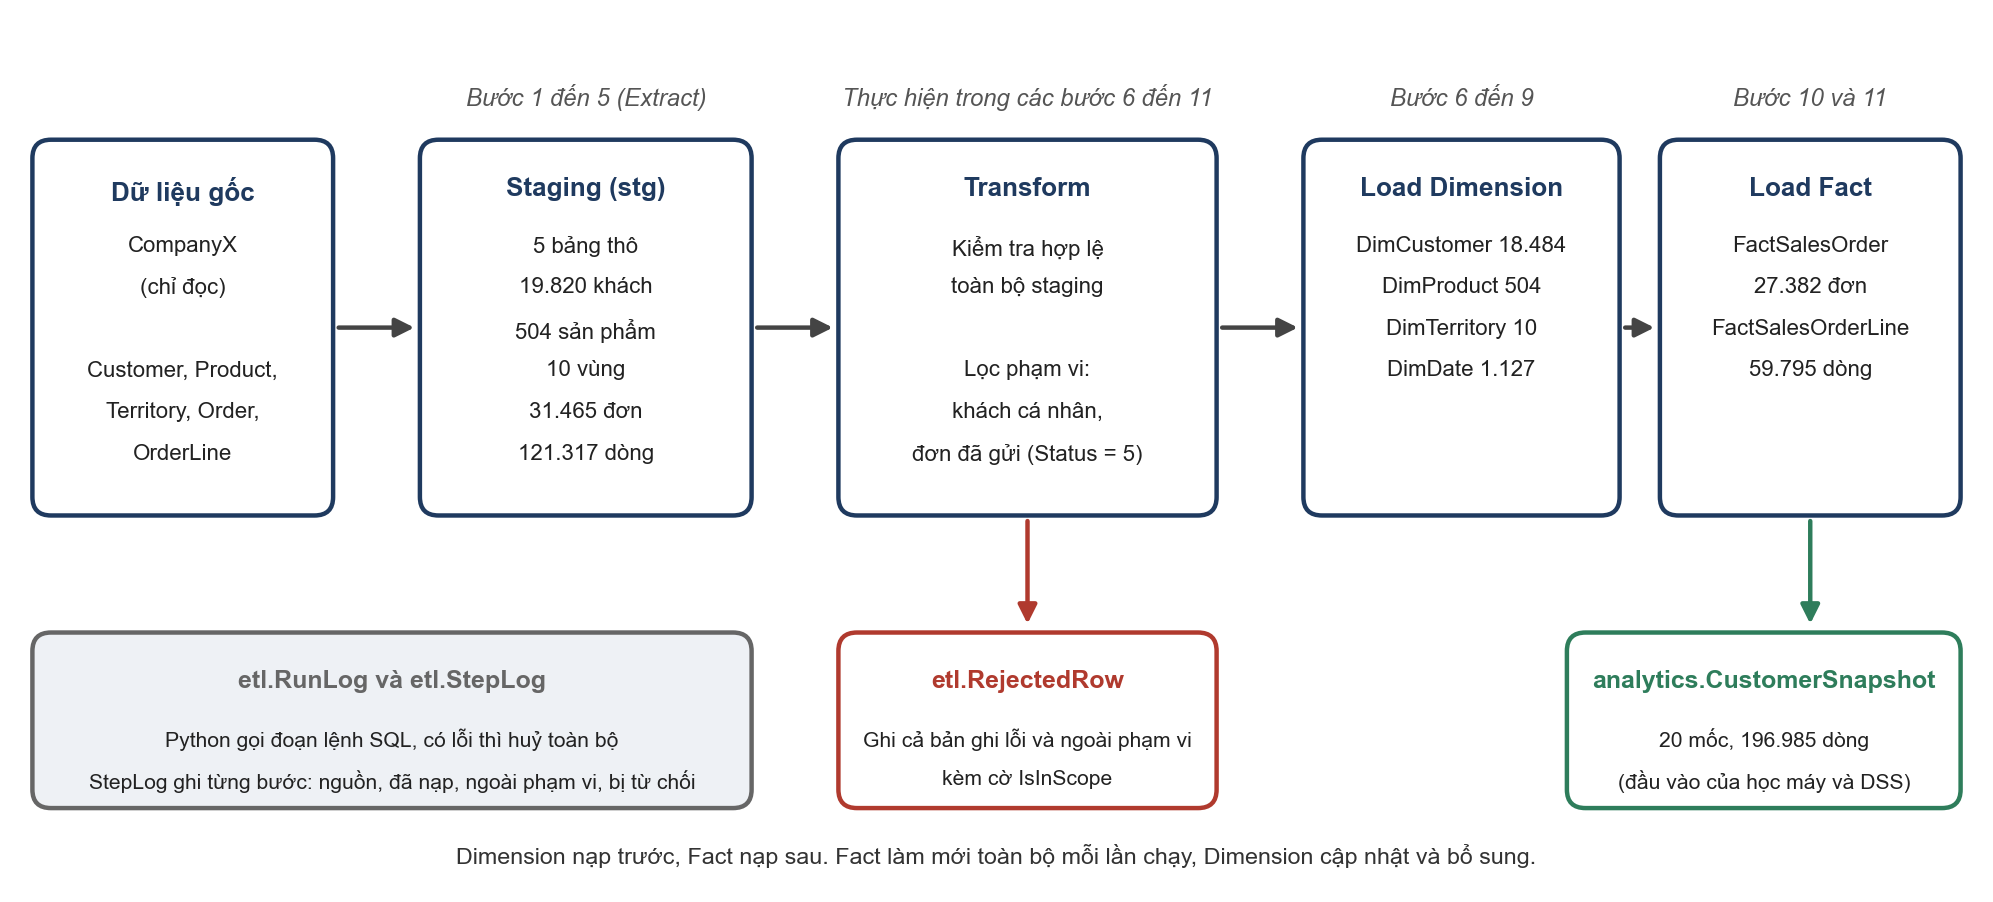
\includegraphics[width=0.8\textwidth]{etl_luong.png}
\caption{Luồng ETL từ dữ liệu gốc đến bảng Snapshot}
\label{fig:etlluong}
\end{figure}

\subsection{Khảo sát dữ liệu nguồn}
Trước khi thiết kế, nhóm xem kỹ cơ sở dữ liệu gốc bằng truy vấn SQL (Bảng~\ref{tab:khaosat}).

\begin{table}[H]
\centering
\caption{Kết quả xem dữ liệu gốc và quyết định của nhóm}
\label{tab:khaosat}
\footnotesize
\begin{tabular}{p{2.7cm}p{7.8cm}p{4.2cm}}
\toprule
Câu hỏi & Nhóm tìm thấy & Nhóm quyết định \\
\midrule
Dữ liệu là gì & CompanyX sản xuất xe đạp, đồng thời bán linh kiện, phụ kiện và trang phục. Cơ sở dữ liệu có 72 bảng về sản xuất, mua hàng và bán hàng. Các đơn được đặt từ 31/05/2011 đến 30/06/2014. Người mua gồm khách cá nhân (cột \texttt{PersonID} có giá trị) và cửa hàng đại lý (cột \texttt{StoreID} có giá trị) & Chỉ dùng phần bán hàng và khách cá nhân \\
Các bảng nối nhau ra sao & Mỗi đơn có một dòng tổng và nhiều dòng chi tiết (mỗi dòng là một sản phẩm), nối bằng \texttt{SalesOrderID}. Sản phẩm thuộc một nhóm nhỏ, nhóm nhỏ thuộc một nhóm lớn & Làm một bảng cho đơn, một bảng cho dòng chi tiết, và các bảng mô tả \\
Điểm cần lưu ý & \texttt{Status} bằng 5 nghĩa là đơn đã gửi. Ngày gửi luôn sau ngày đặt đúng 7 ngày. Tổng tiền đơn bằng tiền hàng cộng thuế và phí vận chuyển. Tháng 6/2014 có 930 đơn nhưng không có xe đạp nào. Có 6 đơn và 75 dòng chi tiết sai quy tắc & Chỉ lấy đơn đã gửi. Chỉ dùng ngày chốt $T$ khi dữ liệu đã có đến ngày $T+97$ (90 ngày theo dõi cộng 7 ngày gửi hàng). Loại các dòng sai quy tắc \\
\bottomrule
\end{tabular}
\end{table}

\subsection{Kiến trúc và luồng xử lý}
Quy trình chỉ đọc dữ liệu gốc, không sửa gì ở đó. Dữ liệu đi qua ba chặng như trong Hình~\ref{fig:etlluong}. Chặng một sao chép nguyên bản sang một vùng tạm gồm năm bảng (gọi là staging, tên \texttt{stg}). Chặng hai kiểm tra và lọc đúng phạm vi cần phân tích. Chặng ba đưa dữ liệu vào bốn bảng mô tả và hai bảng giao dịch của kho. Sau cùng, bảng \texttt{analytics.\allowbreak CustomerSnapshot} tóm tắt cách mua của từng khách để làm đầu vào cho học máy.

Python gọi một đoạn lệnh SQL lưu sẵn tên \texttt{etl.usp\_\allowbreak FullLoad} để làm hết các việc trên. Nếu có lỗi thì mọi thay đổi bị huỷ như chưa từng chạy (transaction). Cách làm này gần với ELT hơn ETL cổ điển: nạp dữ liệu thô vào vùng tạm trước, rồi biến đổi bằng SQL ngay trong SQL Server. Hai bảng \texttt{etl.RunLog} và \texttt{etl.StepLog} ghi lại các lần chạy, đóng vai trò siêu dữ liệu (metadata) của quá trình ETL.

\subsection{Thiết kế kho dữ liệu}
Kho được thiết kế theo mô hình hình sao. Ở giữa là bảng sự kiện (Fact), ghi các giao dịch cần đo. Xung quanh là các bảng chiều (Dimension), cho biết giao dịch đó của ai, mua gì, khi nào, ở đâu. Bảng~\ref{tab:cacbang} liệt kê sáu bảng của kho và Hình~\ref{fig:luocdosao} là sơ đồ. Nhóm đi theo hướng của Kimball: xây trước một kho nhỏ đúng bài toán đang cần (bottom-up), không xây kho chuẩn hoá cho cả công ty như hướng Inmon (top-down). Bảng chiều có phân cấp để xem từ tổng quát đến chi tiết (ngày lên tháng, quý và năm, sản phẩm lên nhóm nhỏ và nhóm lớn, vùng lên quốc gia và nhóm vùng) và gộp sẵn các cấp vào một bảng thay vì tách nhiều bảng nhỏ (hình bông tuyết), nên truy vấn ít phải nối bảng và dễ phân tích nhiều chiều (OLAP).

\begin{table}[H]
\centering
\caption{Sáu bảng của kho \texttt{CompanyX\_DW} và số bản ghi sau ETL}
\label{tab:cacbang}
\small
\begin{tabular}{lp{3.3cm}p{5.6cm}r}
\toprule
Bảng & Mỗi dòng là & Nội dung chính & Số bản ghi \\
\midrule
\texttt{DimCustomer} & Một khách hàng cá nhân & Mã khách, mã cá nhân nguồn, họ tên, mã vùng & 18.484 \\
\texttt{DimDate} & Một ngày & Ngày, tháng, quý, năm & 1.127 \\
\texttt{DimProduct} & Một sản phẩm & Mã sản phẩm nguồn, tên, danh mục con, danh mục & 504 \\
\texttt{DimTerritory} & Một vùng bán hàng & Mã vùng nguồn, tên vùng, quốc gia, nhóm vùng & 10 \\
\texttt{FactSalesOrder} & Một đơn hàng & SubTotal, TaxAmt, Freight, TotalDue & 27.382 \\
\texttt{FactSalesOrderLine} & Một dòng chi tiết đơn & OrderQty, UnitPrice, UnitPriceDiscount, LineTotal & 59.795 \\
\bottomrule
\end{tabular}

\end{table}

\begin{itemize}
    \item \textbf{Phạm vi.} Kho chỉ phục vụ bài toán khách có quay lại mua hay không, nên chỉ chứa khách cá nhân và đơn đã gửi.
    \item \textbf{Hai bảng sự kiện.} Một bảng mỗi dòng là một đơn, một bảng mỗi dòng là một sản phẩm trong đơn. Thuế, phí vận chuyển và tổng tiền tính cho cả đơn nên chỉ để ở bảng đơn, để khi cộng theo sản phẩm không bị tính hai lần.
    \item \textbf{Số liệu đo.} Tiền hàng (\texttt{SubTotal}), thuế (\texttt{TaxAmt}), phí vận chuyển (\texttt{Freight}), tổng tiền (\texttt{TotalDue}), số lượng (\texttt{OrderQty}) và thành tiền của dòng (\texttt{LineTotal}) cộng lại được. Đơn giá (\texttt{UnitPrice}) và tỷ lệ giảm giá (\texttt{UnitPriceDiscount}) thì không cộng được.
    \item \textbf{Mã số và quy tắc.} Mỗi bảng mô tả có một mã số tự tăng do kho tự tạo (khoá thay thế), không dùng mã của hệ thống gốc. Riêng bảng ngày dùng mã dạng \texttt{YYYYMMDD}. Kho có 6 khoá chính (mã không trùng của mỗi bảng), 7 khoá ngoại (liên kết giữa các bảng) và 7 quy tắc chặn dữ liệu sai, ví dụ số lượng phải dương, giảm giá từ 0 đến 1. \texttt{SalesOrderID} có ở cả hai bảng sự kiện để nối đơn với các dòng chi tiết của nó. Cột vùng ở bảng đơn được phép trống, nhưng không đơn nào thiếu vùng nên kho không cần dòng ``không xác định''.
    \item \textbf{Khi thông tin thay đổi.} Khi khách, sản phẩm hay vùng đổi thông tin, kho ghi đè giá trị mới lên giá trị cũ và không giữ bản cũ (slowly changing dimension kiểu 1), vì dữ liệu gốc chỉ lưu giá trị hiện tại.
\end{itemize}

\begin{figure}[H]
\centering
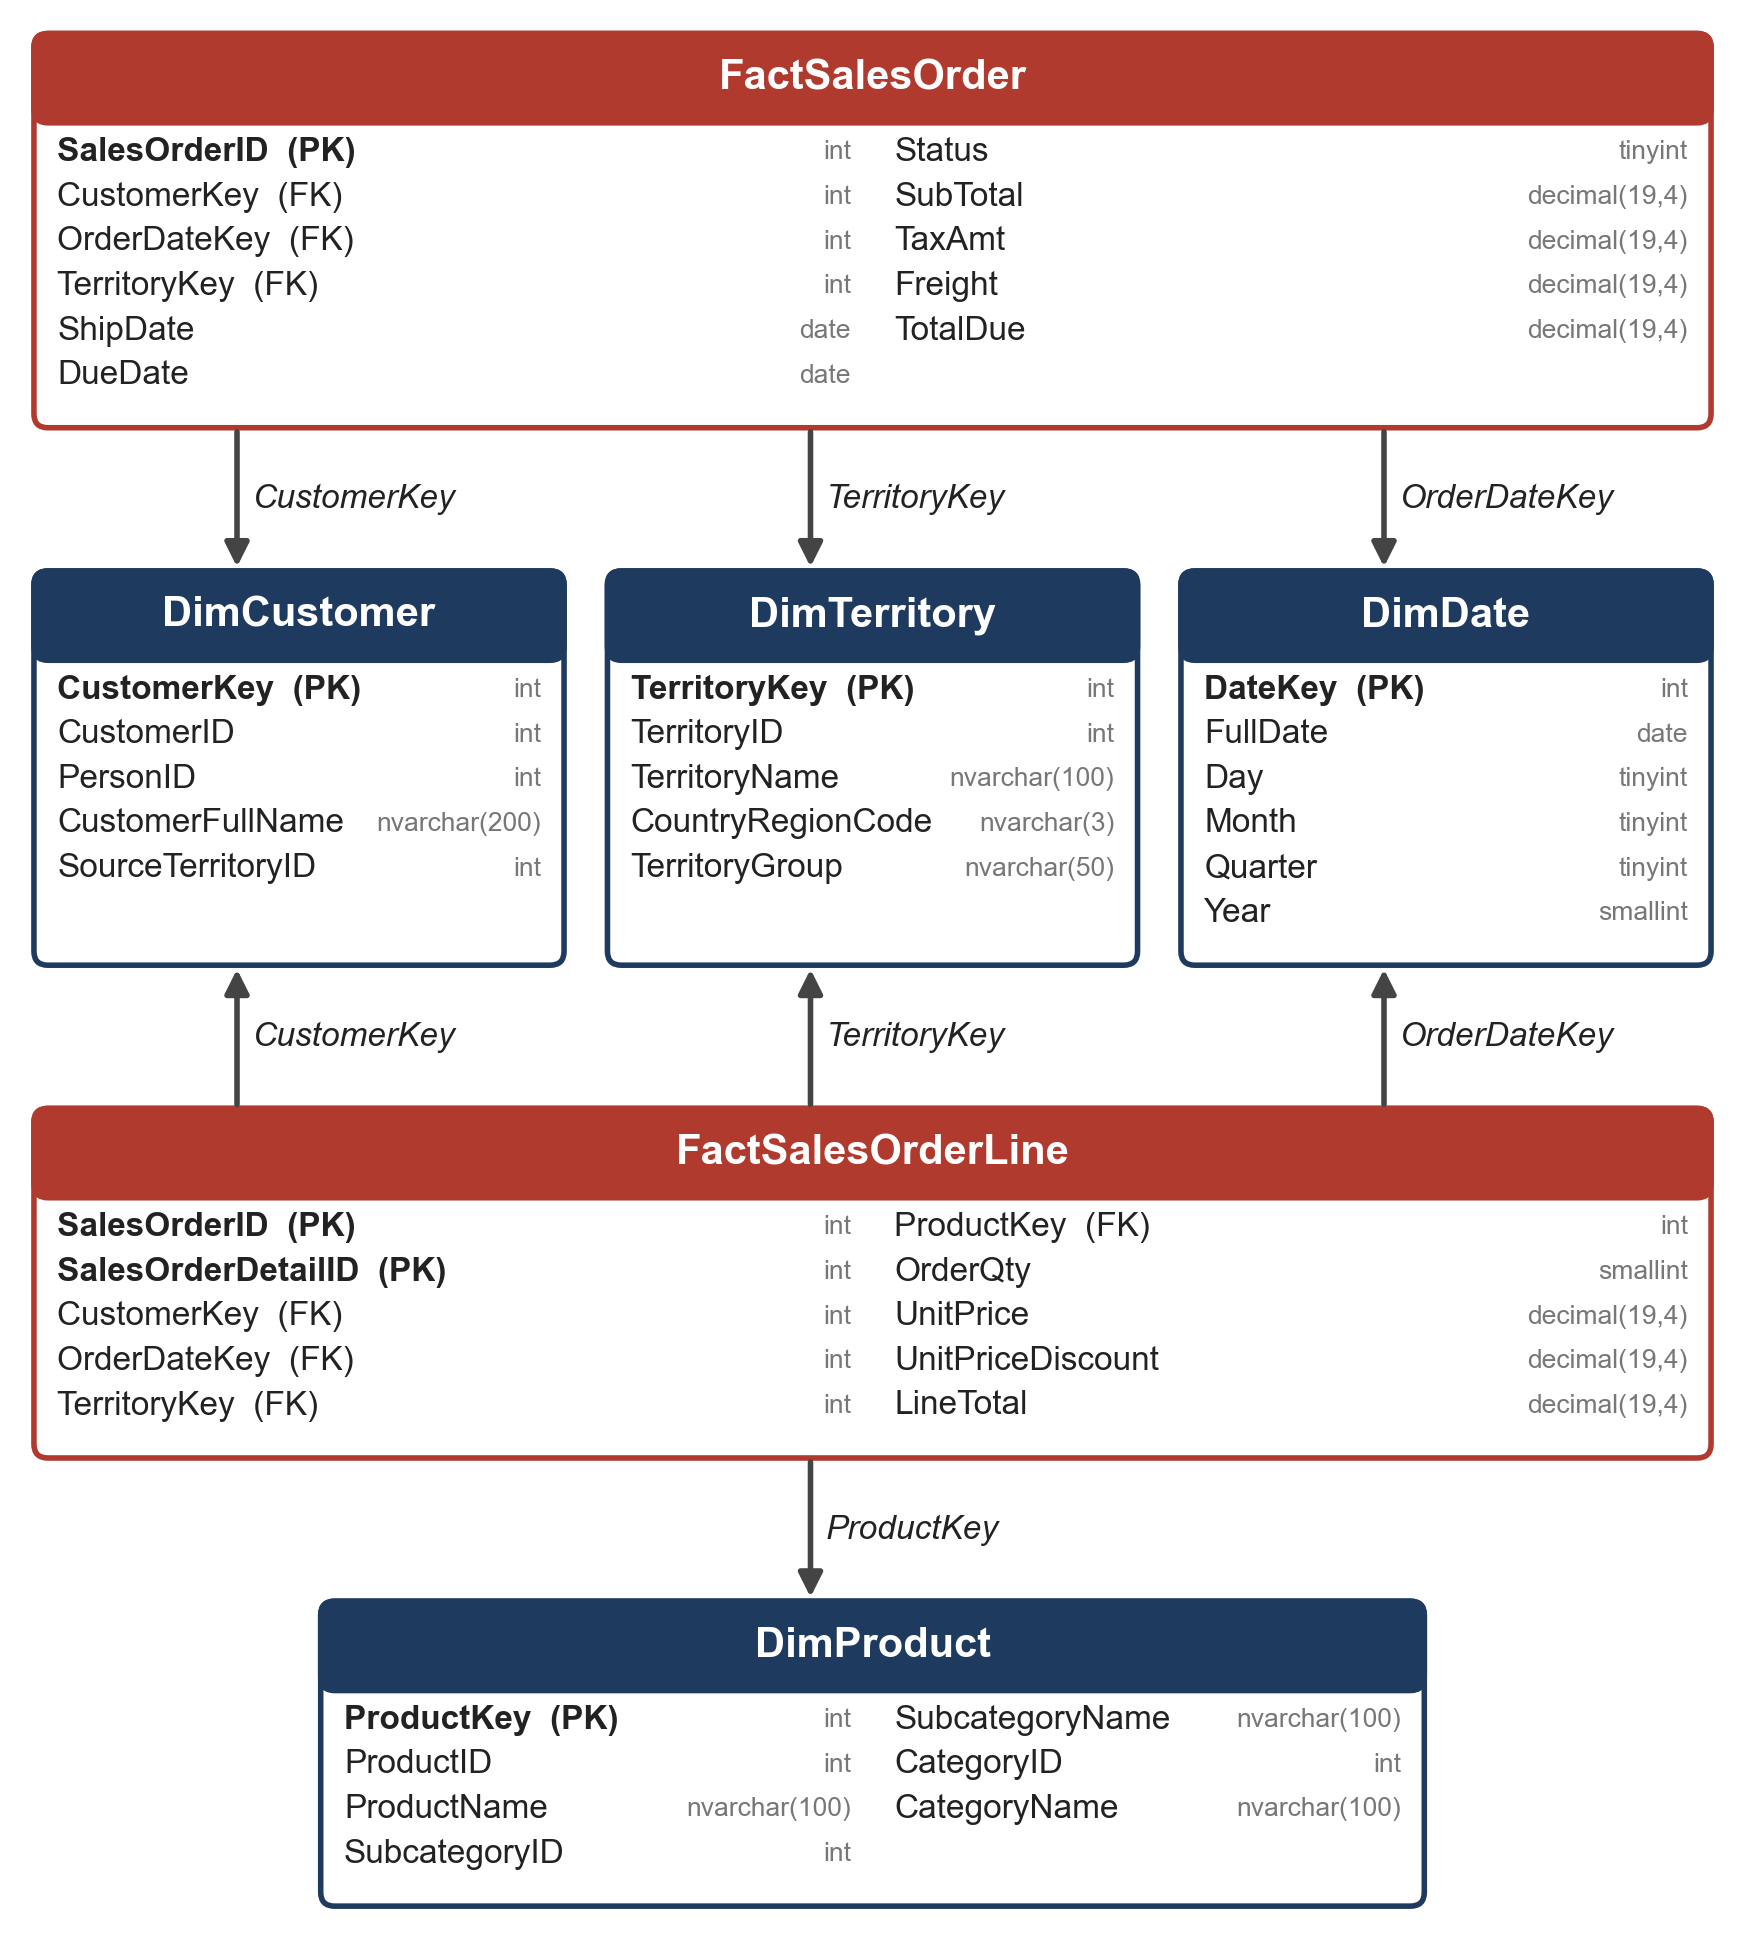
\includegraphics[width=0.5\textwidth]{luoc_do_sao.png}
\caption{Sơ đồ hình sao của kho \texttt{CompanyX\_DW}}
\label{fig:luocdosao}
\end{figure}
\subsection{Dữ liệu gốc đi vào kho như thế nào}
Bảng~\ref{tab:anhxa} cho biết dữ liệu từ bảng gốc nào đi vào bảng nào của kho và được xử lý ra sao.

\begin{table}[H]
\centering
\caption{Dữ liệu từ \texttt{CompanyX} (gốc) đi vào \texttt{CompanyX\_DW} (kho)}
\label{tab:anhxa}
\footnotesize
\begin{tabular}{p{3.8cm}p{3.0cm}p{7.6cm}}
\toprule
Bảng gốc & Bảng trong kho & Cách xử lý \\
\midrule
\texttt{Sales.Customer}, \texttt{Person.Person} & \texttt{DimCustomer} & Chỉ lấy khách cá nhân, ghép họ tên thành một cột \\
\texttt{Product}, \texttt{Product\allowbreak Subcategory}, \texttt{Product\allowbreak Category} & \texttt{DimProduct} & Ghép sản phẩm với nhóm nhỏ và nhóm lớn, vẫn giữ sản phẩm chưa phân loại \\
\texttt{Sales.SalesTerritory} & \texttt{DimTerritory} & Lấy mã vùng, quốc gia, nhóm vùng và đổi tên cột cho rõ nghĩa \\
\texttt{OrderDate} của đơn & \texttt{DimDate} & Tạo đủ mọi ngày từ ngày đặt đầu tiên đến cuối cùng, mã dạng \texttt{YYYYMMDD} \\
\texttt{Sales.\allowbreak SalesOrderHeader} & \texttt{Fact\allowbreak SalesOrder} & Chỉ lấy đơn đã gửi (\texttt{Status} bằng 5), tìm mã khách, ngày, vùng trong các bảng mô tả (vùng được để trống) \\
\texttt{Sales.\allowbreak SalesOrderDetail} & \texttt{Fact\allowbreak SalesOrderLine} & Chỉ lấy dòng của các đơn đã vào kho, tìm mã sản phẩm, giữ số lượng, đơn giá, giảm giá \\
\bottomrule
\end{tabular}
\end{table}

\subsection{Luồng ETL 11 bước}
Bảng~\ref{tab:etl11} liệt kê 11 bước của lần chạy cuối. Ở mỗi bước, số bản ghi ở cột ``Nguồn'' bằng ``Nạp'' cộng ``Loại'' cộng ``Từ chối''. Loại là bản ghi đúng nhưng không thuộc phạm vi phân tích (ví dụ khách là đại lý). Từ chối là bản ghi thuộc phạm vi nhưng bị lỗi dữ liệu.

\begin{table}[H]
\centering
\caption{Mười một bước của lần chạy ETL cuối}
\label{tab:etl11}
\footnotesize
{\setlength{\tabcolsep}{3.5pt}\begin{tabular}{rlp{4.0cm}rrrr}
\toprule
Bước & Tên bước & Việc làm & Nguồn & Nạp & Loại & Từ chối \\
\midrule
1 & \texttt{Extract.Customer} & Trích bảng khách hàng và họ tên vào staging & 19.820 & 19.820 & 0 & 0 \\
2 & \texttt{Extract.Product} & Trích sản phẩm cùng danh mục con và danh mục & 504 & 504 & 0 & 0 \\
3 & \texttt{Extract.Territory} & Trích vùng bán hàng & 10 & 10 & 0 & 0 \\
4 & \texttt{Extract.Order} & Trích đầu đơn hàng, chưa lọc & 31.465 & 31.465 & 0 & 0 \\
5 & \texttt{Extract.OrderLine} & Trích dòng chi tiết đơn, chưa lọc & 121.317 & 121.317 & 0 & 0 \\
6 & \texttt{Load.DimCustomer} & Cập nhật và bổ sung khách cá nhân & 19.820 & 18.484 & 1.336 & 0 \\
7 & \texttt{Load.DimProduct} & Cập nhật và bổ sung sản phẩm & 504 & 504 & 0 & 0 \\
8 & \texttt{Load.DimTerritory} & Cập nhật và bổ sung vùng & 10 & 10 & 0 & 0 \\
9 & \texttt{Load.DimDate} & Sinh lịch liên tục theo ngày đặt & 1.127 & 1.127 & 0 & 0 \\
10 & \texttt{Load.FactSalesOrder} & Kiểm tra rồi nạp đơn đã gửi của khách cá nhân & 31.465 & 27.382 & 4.083 & 0 \\
11 & \texttt{Load.FactSalesOrderLine} & Nạp dòng chi tiết của các đơn đã nạp & 121.317 & 59.795 & 61.522 & 0 \\
\bottomrule
\end{tabular}
}
\end{table}

\textbf{Bước 1 đến 5, lấy dữ liệu.} Sao chép nguyên bản năm bảng gốc vào vùng tạm, chưa lọc gì. Mỗi lần chạy xoá vùng tạm rồi sao chép lại.

\textbf{Kiểm tra và loại.} Trước khi lọc, nhóm kiểm tra dữ liệu ở vùng tạm: mã liên kết, ngày tháng, số tiền, số lượng, và hai phép tính tiền sau phải khớp (cho phép lệch 0,01).
\begin{align*}
\text{TotalDue} &= \text{SubTotal} + \text{TaxAmt} + \text{Freight}, \\
\text{LineTotal} &= \text{OrderQty} \times \text{UnitPrice} \times (1 - \text{UnitPriceDiscount}).
\end{align*}
Bản ghi sai được ghi vào bảng \texttt{etl.RejectedRow} kèm lý do. Nếu một dòng chi tiết sai thì cả đơn bị loại, để tổng các dòng luôn bằng tổng của đơn. Lần chạy cuối có 6 đơn và 75 dòng chi tiết sai, nhưng đều không thuộc phạm vi phân tích nên không có bản ghi nào trong phạm vi bị từ chối.

\textbf{Bước 6 đến 11, đưa vào kho.} Các bảng mô tả nạp trước, các bảng giao dịch nạp sau. Bảng mô tả chỉ cập nhật và thêm dòng nên mã số không đổi giữa các lần chạy. Phần ngoài phạm vi gồm 1.336 khách, 4.083 đơn và 61.522 dòng chi tiết. Hai bảng giao dịch được xoá hết rồi nạp lại mỗi lần chạy, vì dữ liệu của đề tài là bản sao lưu cố định. Lần chạy cuối ngày 31/10/2026 mất 2 giây và thành công (\texttt{SUCCESS}).

\subsection{Bảng Customer Snapshot}
Sau khi nạp kho, một đoạn lệnh riêng tạo bảng \texttt{analytics.\allowbreak CustomerSnapshot}, nằm ngoài sơ đồ hình sao. Mỗi dòng là tình trạng của một khách vào một ngày chốt (gọi là mốc), nhận diện bằng \texttt{CustomerID} và \texttt{SnapshotDate}. Bảng này là đầu vào của mô hình học máy. Có 19 mốc trong quá khứ (ngày 1 và 15 hằng tháng, từ 01/06/2013 đến 01/03/2014) và một mốc chấm điểm, tức ngày dùng để dự đoán cho khách hiện tại, là 08/07/2014. Tổng cộng 196.985 dòng. Chỉ số tại mốc $T$ chỉ tính từ các đơn đã đặt và đã gửi trước $T$, để mô hình không biết trước tương lai.

\subsection{Quản lý và kiểm soát chất lượng kho}
Thiết kế kho ở các mục trên cần đi kèm cách vận hành và kiểm soát kho. Các việc quản lý này đang nằm ở nhiều chương, nên mục này gom lại:
\begin{itemize}
    \item \textbf{Siêu dữ liệu và nhật ký ETL.} Bảng \texttt{etl.RunLog} ghi từng lần chạy, \texttt{etl.StepLog} ghi từng bước, \texttt{etl.RejectedRow} ghi bản ghi bị từ chối kèm lý do (Bảng~\ref{tab:etl11}).
    \item \textbf{Chiến lược làm mới.} Mỗi lần chạy nạp lại toàn bộ (full reload) bằng \texttt{etl.usp\_\allowbreak FullLoad}, trong một transaction. Nếu có lỗi, mọi thay đổi bị huỷ (rollback) như chưa từng chạy. Hạn chế của cách này nêu ở mục Giới hạn cuối chương.
    \item \textbf{Quản lý phiên bản mô hình và điểm.} Mỗi mô hình có một phiên bản trong \texttt{analytics.\allowbreak ModelRegistry}, điểm của từng khách được lưu kèm phiên bản đã chấm (mục~\ref{sec:chamdiem}).
    \item \textbf{Phân quyền theo vai trò.} Ba vai trò dùng DSS có quyền khác nhau (Bảng~\ref{tab:quyen}, mục~\ref{sec:vaitro}). Bản demo chưa có đăng nhập, vai trò chỉ chọn ở thanh bên để minh hoạ.
\end{itemize}
Về kiểm soát chất lượng, nhóm so sánh dữ liệu gốc với kho bằng câu truy vấn SQL, ở hai lớp. Lớp một gồm 44 phép kiểm tra sau khi nạp (Bảng~\ref{tab:kt44}). Ví dụ tổng tiền hàng là 29.052.549,9450 và tổng tiền đơn là 32.103.068,4755, giống nhau ở dữ liệu gốc và kho (lệch không quá 0,01). Lớp hai gồm 21 phép kiểm tra riêng cho bảng Snapshot (Bảng~\ref{tab:kt21}), tính lại chỉ số từ dữ liệu gốc rồi so với kho. Tất cả đều đạt.

\begin{table}[H]
\centering
\caption{Kết quả 44 phép kiểm tra sau khi nạp kho}
\label{tab:kt44}
\footnotesize
\begin{tabular}{lrr}
\toprule
Nhóm kiểm tra & Số phép & Kết quả \\
\midrule
Số lượng bản ghi (đầy đủ) & 8 & 8 đạt \\
Mã định danh nguồn & 8 & 8 đạt \\
Khoá và quan hệ (duy nhất, nhất quán) & 6 & 6 đạt \\
Phạm vi và ánh xạ (hợp lệ) & 8 & 8 đạt \\
Giá trị tài chính (chính xác) & 4 & 4 đạt \\
Bản ghi bất thường & 6 & 6 đạt \\
Nhật ký ETL (truy vết) & 4 & 4 đạt \\
\textbf{Tổng cộng} & \textbf{44} & \textbf{44 đạt, 0 lỗi} \\
\bottomrule
\end{tabular}

\end{table}

\begin{table}[H]
\centering
\caption{Kết quả 21 phép kiểm tra bảng Customer Snapshot}
\label{tab:kt21}
\footnotesize
\begin{tabular}{lrr}
\toprule
Nhóm kiểm tra & Số phép & Kết quả \\
\midrule
Lịch mốc & 4 & 4 đạt \\
Độ phủ khách & 4 & 4 đạt \\
Miền giá trị & 4 & 4 đạt \\
Tính lại RFM từ nguồn & 5 & 5 đạt \\
Tính lại thuộc tính sản phẩm & 4 & 4 đạt \\
\textbf{Tổng cộng} & \textbf{21} & \textbf{21 đạt, 0 lỗi} \\
\bottomrule
\end{tabular}

\end{table}

\subsection{Giới hạn}
\begin{itemize}
    \item ETL chỉ chạy khi có người bấm chạy, chưa tự chạy theo lịch, và chưa thử trường hợp lỗi giữa chừng. Một transaction cho toàn bộ ETL chỉ hợp với dữ liệu nhỏ (2 giây), dữ liệu lớn cần chia nhỏ.
    \item Chỉ có một nguồn dữ liệu, và kho ghi đè thông tin cũ nên không xem lại được thông tin trước đây.
    \item Chỉ ngày đặt hàng nối với bảng ngày.
\end{itemize}

\clearpage
% Chương Tiền xử lý và khám phá dữ liệu (EDA)
% Bảng trong latex/bang/ do python/tao_bang_tex_eda.py sinh từ results/, hình do python/ve_hinh_eda.py vẽ.
% Không sửa tay số liệu trong latex/bang/, chạy lại hai script trên.
\section{Tiền xử lý và khám phá dữ liệu}

Chương này chuẩn bị dữ liệu cho bước học máy, tức bước chọn và biến đổi dữ liệu nằm giữa kho dữ liệu và bước khai phá. Các việc nhóm làm thuộc bốn nhóm tiền xử lý quen thuộc: làm sạch (kiểm tra giá trị thiếu, giữ ngoại lai), tích hợp (đã làm ở ETL, Chương 3), biến đổi (xây dựng thuộc tính, xác định khách rời bỏ, chia khoảng, chuẩn hoá) và rút gọn (thử bỏ bớt thuộc tính). Các con số lấy từ kho \texttt{CompanyX\_DW} và các tệp kết quả của chuỗi phân tích.

\subsection{Dữ liệu đầu vào sau ETL}
Kho có 18.484 khách cá nhân, 27.382 đơn và 59.795 dòng chi tiết (Bảng~\ref{tab:cacbang}). Trong đó 18.360 khách có ít nhất một đơn đã gửi, còn 124 khách chưa có đơn đã gửi nào nên không đưa vào phân tích. Chương 1 tính cả 635 đại lý (tổng 18.995 khách có đơn đã giao) nên tỷ lệ khách chỉ mua một lần là 61,21\%, còn chương này chỉ tính khách cá nhân nên là 63,2\%. Bảng \texttt{analytics.\allowbreak CustomerSnapshot} có 196.985 dòng tại 20 mốc và đã qua các phép kiểm tra ở Bảng~\ref{tab:kt44} và~\ref{tab:kt21}.

\subsection{Khám phá dữ liệu tại mốc chấm điểm}
Mốc chấm điểm là ngày 08/07/2014, ngày dùng để dự đoán cho khách hiện tại, với 18.360 khách. Phần này xem dữ liệu mà người ra quyết định sẽ nhìn thấy.

\subsubsection{Các thuộc tính và phân bố}
Mỗi khách tại mốc $T$ được mô tả bằng 11 thuộc tính (Bảng~\ref{tab:thuoctinh}), gồm 10 cột của bảng Snapshot và BikeBuyer suy ra từ Share\_Bikes, chỉ tính từ các đơn đã gửi trước $T$ nên không chứa thông tin của tương lai. Việc tính các thuộc tính này từ đơn hàng là bước xây dựng thuộc tính (attribute construction) và tổng hợp (aggregation). Không thuộc tính nào bị thiếu giá trị. AOV không đưa vào mô hình phân lớp, chỉ dùng để mô tả và để tính giá trị khách $v_i$ trong DSS (mục 6.2).

\begin{table}[H]
\centering
\caption{Các thuộc tính của khách tại mốc $T$ (tính từ đơn đã gửi trước $T$)}
\label{tab:thuoctinh}
\footnotesize
\begin{tabular}{p{4.4cm}p{10cm}}
\toprule
Thuộc tính & Ý nghĩa \\
\midrule
Recency & Số ngày từ lần đặt hàng gần nhất đến $T$ \\
Frequency & Số đơn đã gửi trước $T$ \\
Monetary & Tổng tiền các đơn đó (\texttt{TotalDue}, đã gồm thuế và phí vận chuyển), tính bằng USD \\
Orders90, Orders180 & Số đơn đặt trong 90 ngày và 180 ngày gần nhất trước $T$ \\
Tenure & Số ngày từ đơn đầu tiên đến $T$ (khách đã gắn bó bao lâu) \\
Share\_Bikes, Share\_Accessories, Share\_Clothing & Tỷ trọng tiền mua xe đạp, phụ kiện, trang phục trong tổng tiền mua của khách \\
NSub & Số nhóm sản phẩm nhỏ khác nhau mà khách đã mua \\
BikeBuyer & Bằng 1 nếu tiền mua xe đạp chiếm trên một nửa tổng tiền mua của khách (Share\_Bikes $> 0{,}5$), tức khách đã mua xe đạp \\
AOV & Tiền hàng trung bình mỗi đơn (\texttt{SubTotal}), không vào mô hình, dùng tính $v_i$ ở DSS \\
\bottomrule
\end{tabular}
\end{table}

Bảng~\ref{tab:thongke} (Monetary và AOV tính bằng USD, Recency và Tenure tính bằng ngày) và Hình~\ref{fig:phanbo} cho thấy ba thuộc tính Recency, Frequency và Monetary (gọi tắt là R, F, M) đều lệch về một phía.
\begin{itemize}
    \item \textbf{Recency:} trung vị 176 ngày, nhưng có khách đã 1.134 ngày chưa mua lại.
    \item \textbf{Frequency:} 11.595 khách (63,2\%) chỉ có một đơn.
    \item \textbf{Monetary:} trung bình 1.748,53 USD nhưng trung vị chỉ 316,97 USD, nên cần xem cả hai con số. Trên trục logarit có hai đỉnh tách biệt, khớp với việc khách có mua xe đạp hay không: 9.270 khách chưa mua xe đạp có trung vị 55,50 USD, 9.090 khách đã mua có trung vị 2.783,46 USD.
\end{itemize}
Các giá trị rất lớn như 14.691,40 USD hay 28 đơn của một khách là giao dịch có thật, thuộc nhóm khách giá trị cao, nên nhóm giữ nguyên, không loại hay làm mịn. Khi chia khoảng (mục 4.5) chúng tự rơi vào khoảng cao nhất nên không làm lệch mô hình.

\begin{table}[H]
\centering
\caption{Thống kê sáu thuộc tính của 18.360 khách tại mốc 08/07/2014}
\label{tab:thongke}
\footnotesize
\resizebox{\textwidth}{!}{\begin{tabular}{lrrrrrrr}
\toprule
Thuộc tính & Trung bình & Độ lệch chuẩn & Nhỏ nhất & Q1 & Trung vị & Q3 & Lớn nhất \\
\midrule
Recency & 198,58 & 148,54 & 8 & 94 & 176 & 272 & 1.134 \\
Frequency & 1,49 & 1,10 & 1 & 1 & 1 & 2 & 28 \\
Monetary & 1.748,53 & 2.334,78 & 2,53 & 55,22 & 316,97 & 2.754,01 & 14.691,40 \\
AOV & 914,41 & 1.042,60 & 2,29 & 39,98 & 163,99 & 1.775,47 & 3.578,27 \\
Tenure & 354,27 & 276,85 & 8 & 148 & 277 & 480 & 1.134 \\
NSub & 2,42 & 1,27 & 1 & 2 & 2 & 3 & 12 \\
\bottomrule
\end{tabular}
}
\end{table}

\begin{figure}[!htbp]
\centering
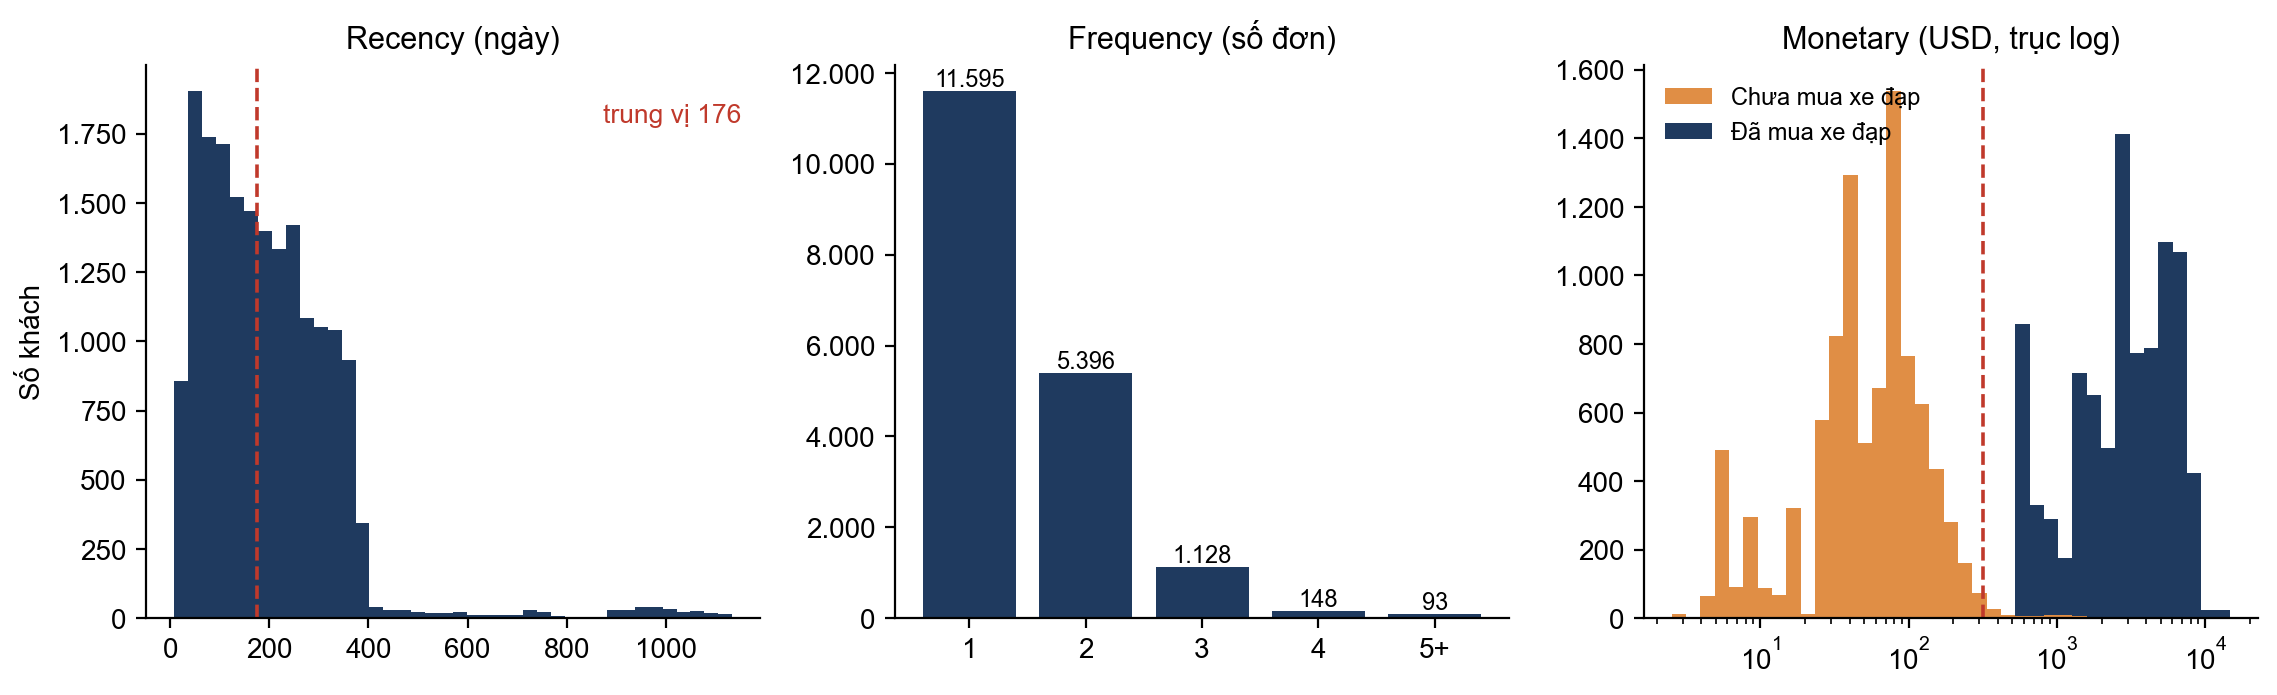
\includegraphics[width=0.85\textwidth]{eda_phan_bo_rfm.png}
\caption{Phân bố Recency, Frequency và Monetary}
\label{fig:phanbo}
\end{figure}

\subsubsection{Quan hệ giữa các thuộc tính}
Hình~\ref{fig:tuongquan} cho hệ số tương quan hạng (Spearman) giữa sáu thuộc tính số: càng gần 1 thì hai thuộc tính càng cùng tăng giảm, càng gần 0 thì càng không liên quan.
\begin{itemize}
    \item Monetary và AOV gần như đi cùng nhau (0,96), nên AOV không cho thêm thông tin.
    \item Recency gần như không liên quan đến Monetary (0,03) và Frequency ($-0{,}18$), nên R, F, M mô tả ba khía cạnh khác nhau.
    \item Các cặp từ 0,7 trở lên trong 11 thuộc tính của mô hình đều gần như trùng nghĩa, ví dụ Share\_Bikes với BikeBuyer (0,87).
\end{itemize}

\begin{figure}[!htbp]
\centering
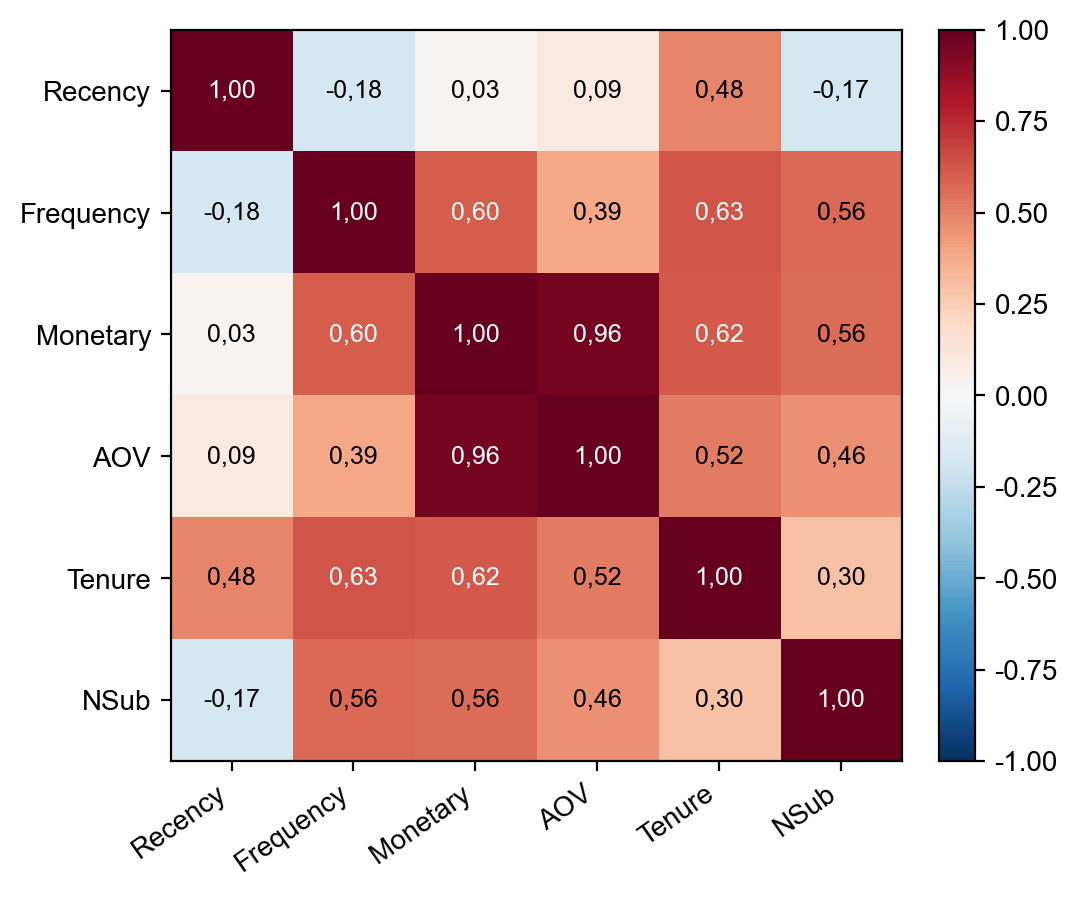
\includegraphics[width=0.55\textwidth]{eda_tuong_quan.png}
\caption{Tương quan hạng Spearman giữa sáu thuộc tính số tại mốc 08/07/2014}
\label{fig:tuongquan}
\end{figure}

\subsubsection{Xu hướng theo thời gian}
Hình~\ref{fig:xuhuongthang} cho thấy số đơn tăng vọt từ tháng 7/2013: khoảng 237 đơn mỗi tháng từ 6/2011 đến 6/2013, rồi khoảng 1.866 đơn mỗi tháng từ 7/2013 đến 5/2014, cao nhất là tháng 5/2014 với 2.209 đơn. Xe đạp chỉ chiếm 15.050 trong 59.795 dòng chi tiết nhưng tạo ra 96,5\% giá trị, còn phụ kiện chiếm nhiều dòng nhất (35.719) nhưng giá trị nhỏ. Tháng 6/2014 bất thường: 930 đơn nhưng không có xe đạp nào, nên doanh thu chỉ khoảng 48,7 nghìn USD. Vì vậy nhóm không dùng tháng 6/2014 để xác định khách rời bỏ.

\begin{figure}[!htbp]
\centering
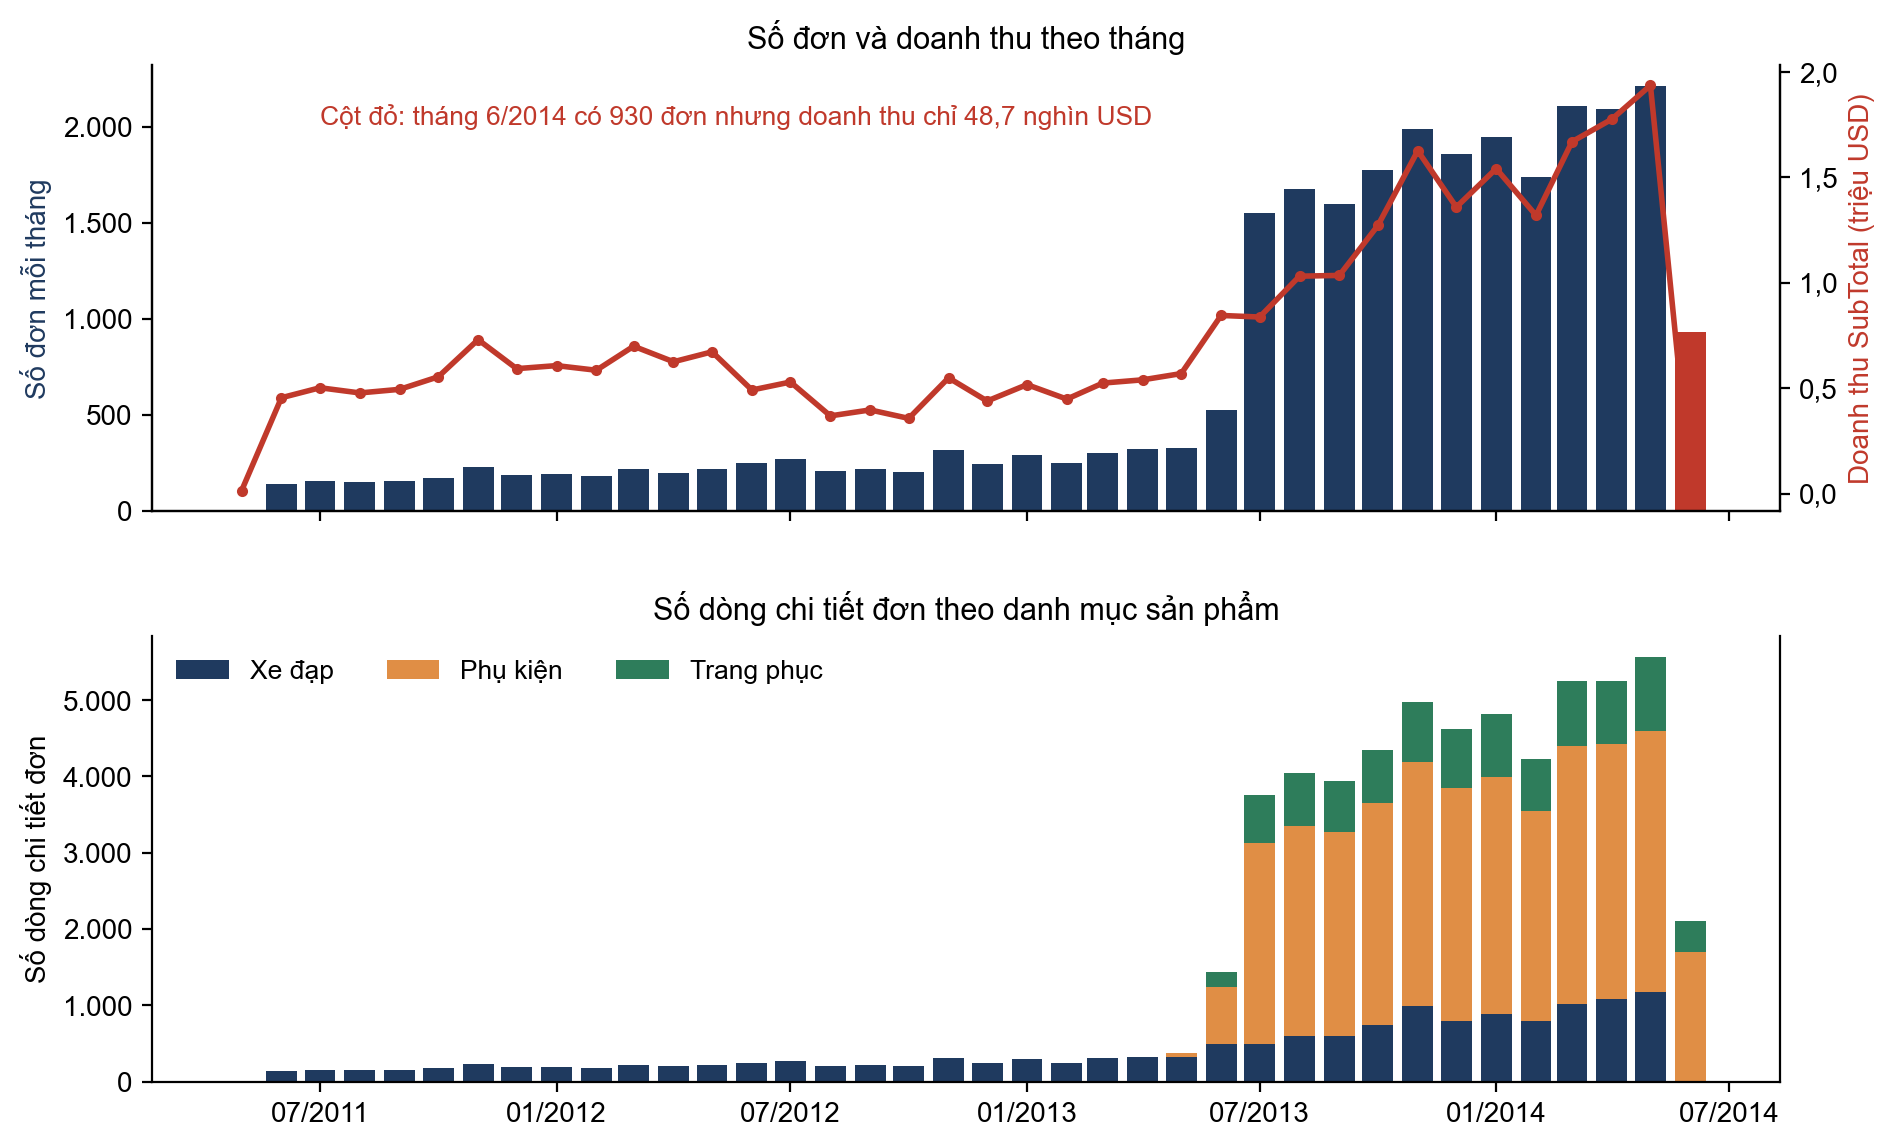
\includegraphics[width=0.75\textwidth]{eda_xu_huong_thang.png}
\caption{Số đơn, doanh thu và số dòng chi tiết theo nhóm sản phẩm của từng tháng}
\label{fig:xuhuongthang}
\end{figure}

\subsubsection{Khách nào mang lại nhiều tiền}
Hình~\ref{fig:pareto} xếp 18.360 khách từ chi tiêu nhiều đến ít. Tiền tập trung vào một số khách nhưng không cực đoan như quy tắc 80/20: 10\% khách đầu mang lại 40,2\% tổng chi tiêu, và cần 28,0\% khách để đạt 80\%. Nhóm chia khách thành ba hạng theo chi tiêu cộng dồn.
\begin{itemize}
    \item \textbf{Hạng A:} 5.137 khách (Monetary từ 2.649,85 USD), tạo ra 80\% tổng chi tiêu.
    \item \textbf{Hạng B:} 2.581 khách (từ 895,40 USD), tạo ra 15\% tiếp theo.
    \item \textbf{Hạng C:} 10.642 khách, chiếm 58,0\% số khách nhưng chỉ mang lại 5\% tổng chi tiêu.
\end{itemize}
Các hạng này dùng ở các chương sau để ưu tiên chăm sóc.

\begin{figure}[!htbp]
\centering
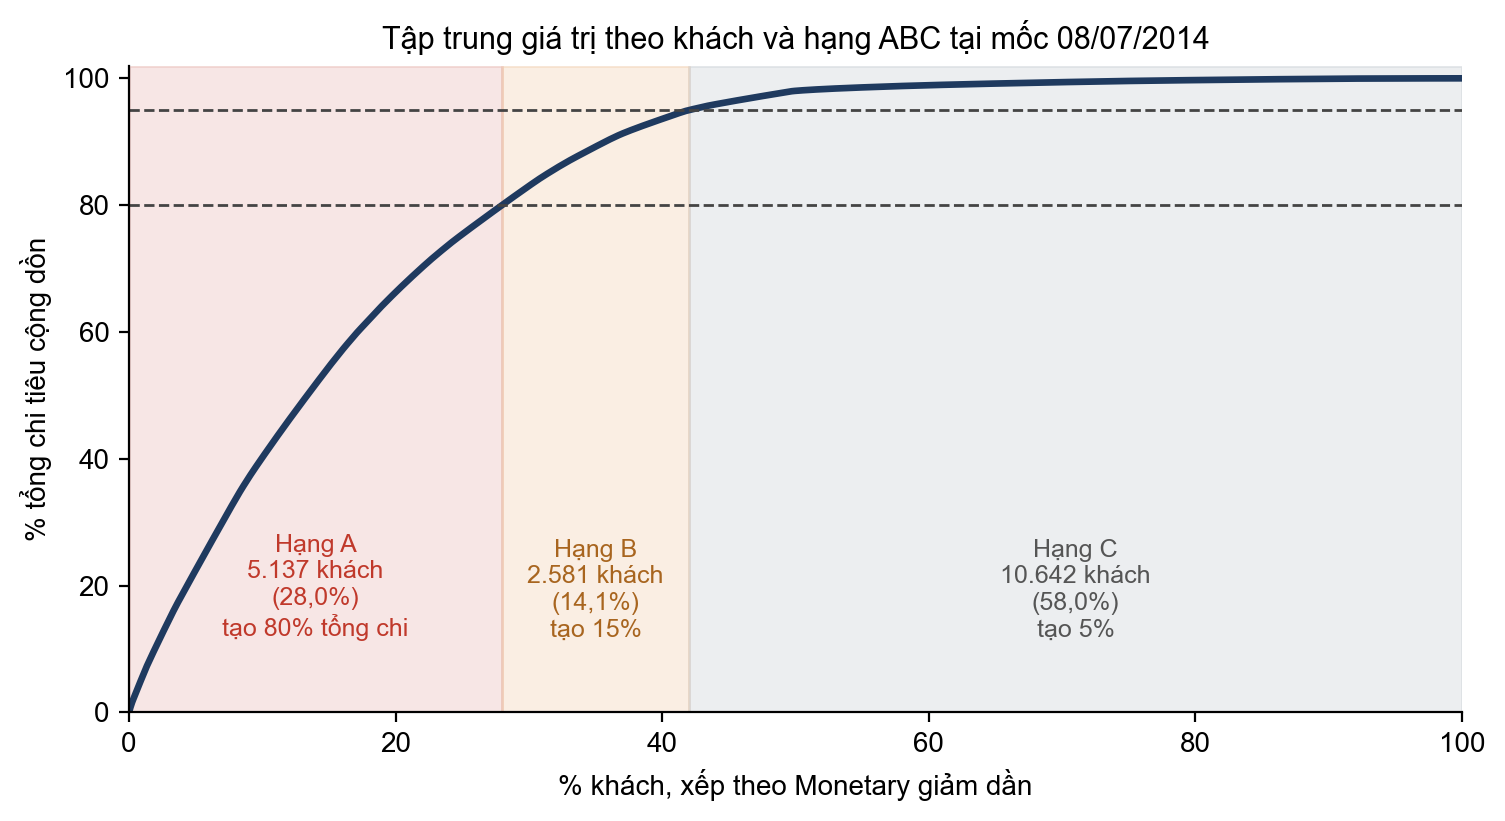
\includegraphics[width=0.65\textwidth]{eda_pareto.png}
\caption{Chi tiêu cộng dồn theo phần trăm khách và ba hạng A, B, C}
\label{fig:pareto}
\end{figure}

\subsection{Xác định khách rời bỏ}
Dữ liệu không có sẵn nhãn rời bỏ nên nhóm tự định nghĩa từ lịch sử mua. Một khách có nhãn $y=1$ (có nguy cơ rời bỏ) nếu sau mốc $T$ khách không đặt đơn nào trong 90 ngày, ngược lại là $y=0$:
\[
y = \begin{cases} 1 & \text{nếu khách không đặt đơn nào trong khoảng } [T,\, T+90) \\ 0 & \text{nếu có đặt ít nhất một đơn.} \end{cases}
\]
Chỉ khách đã có ít nhất một đơn đã gửi trước $T$ mới được gán nhãn. Một mốc $T$ chỉ dùng để huấn luyện mô hình khi đủ hai điều kiện.
\begin{itemize}
    \item \textbf{Đủ thời gian để biết nhãn.} Mốc kiểm tra $E$ phải muộn hơn $T$ ít nhất 97 ngày ($T+97 \leq E$). Lý do là hàng được gửi sau ngày đặt đúng 7 ngày và Snapshot chỉ tính đơn đã gửi, nên đơn đặt ở ngày cuối của 90 ngày ($T+89$) chỉ thấy được từ ngày $T+97$.
    \item \textbf{Không dùng tháng 6/2014.} Cửa sổ 90 ngày phải kết thúc trước 01/06/2014, vì tháng này không có xe đạp.
\end{itemize}
Nhờ vậy 19 mốc từ 01/06/2013 đến 01/03/2014 có nhãn đầy đủ, còn mốc 08/07/2014 chỉ có thuộc tính để dự đoán.

Qua các mốc huấn luyện, số khách tăng từ 5.324 lên 14.167, tỷ lệ $y=1$ luôn quanh 79,3\% đến 82,8\% nhưng cơ cấu khách đổi nhiều: khách chỉ mua một đơn giảm từ 100\% xuống 69,3\%, khách mua từ hai nhóm sản phẩm nhỏ trở lên tăng từ 0\% lên 64,9\%. Vì vậy mô hình được huấn luyện lại ở mỗi kỳ. Tỷ lệ $y=1$ cao cũng nghĩa là một mô hình luôn đoán ``rời bỏ'' đã đúng khoảng 82\%, nên không thể so sánh các mô hình chỉ bằng độ chính xác tổng thể. Nhóm giữ nguyên tỷ lệ này, không lấy mẫu lại hay đổi trọng số hai lớp, vì ở các chương sau xác suất dự đoán được dùng trực tiếp để tính giá trị kinh tế.

\subsection{Chia dữ liệu theo thời gian}
Dữ liệu huấn luyện mô hình và dữ liệu thử mô hình được chia theo thời gian chứ không chia ngẫu nhiên, vì mục tiêu là dự đoán cho tương lai. Mỗi lần thử dùng một cặp mốc $(E \leftarrow T)$, gọi là một fold: mô hình học tại mốc huấn luyện $T$ rồi dự đoán cho khách tại mốc đánh giá $E$ muộn hơn, với $T+97 \leq E$. Bảng~\ref{tab:fold} gồm bốn cặp dùng để phát triển và chọn mô hình, cộng cặp cuối dùng cho lần dự đoán thật ngày 08/07/2014. Hình~\ref{fig:thoigian} vẽ lịch này, thanh màu là cửa sổ 90 ngày và tam giác là mốc đánh giá.

\begin{table}[H]
\centering
\caption{Bốn cặp mốc phát triển và cặp mốc dự đoán thật}
\label{tab:fold}
\footnotesize
\resizebox{\textwidth}{!}{\begin{tabular}{lrrlrrl}
\toprule
Mốc huấn luyện & Số khách & $y=1$ & Mốc đánh giá & Số khách & $y=1$ & Cửa sổ nhãn của mốc huấn luyện \\
\midrule
01/09/2013 & 7.705 & 79,5\% & 15/12/2013 & 11.564 & 81,8\% & 01/09/2013 đến 29/11/2013 \\
01/10/2013 & 8.812 & 79,4\% & 15/01/2014 & 12.617 & 81,8\% & 01/10/2013 đến 29/12/2013 \\
01/11/2013 & 9.898 & 79,4\% & 15/02/2014 & 13.694 & 82,1\% & 01/11/2013 đến 29/01/2014 \\
15/11/2013 & 10.447 & 80,7\% & 01/03/2014 & 14.167 & 82,0\% & 15/11/2013 đến 12/02/2014 \\
01/03/2014 & 14.167 & 82,0\% & 08/07/2014 & 18.360 & -- & 01/03/2014 đến 29/05/2014 \\
\bottomrule
\end{tabular}
}
\end{table}

\begin{figure}[!htbp]
\centering
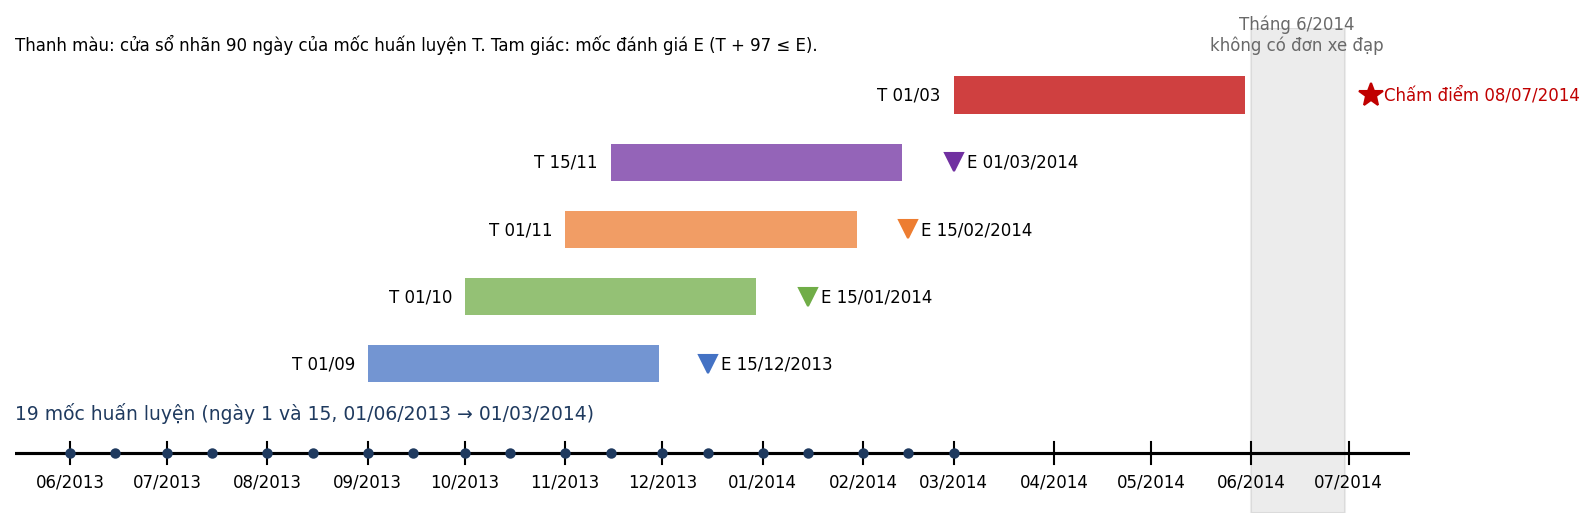
\includegraphics[width=0.8\textwidth]{moc_thoi_gian.png}
\caption{Lịch các mốc huấn luyện, cửa sổ nhãn 90 ngày và mốc đánh giá}
\label{fig:thoigian}
\end{figure}

\subsection{Chia thuộc tính thành khoảng}
Mô hình Naive Bayes làm việc với nhóm giá trị, nên R, F, M được chia thành các khoảng trước khi huấn luyện mô hình. Monetary được chia thành bốn nhóm có số khách xấp xỉ bằng nhau (theo tứ phân vị). Tại mốc huấn luyện 01/03/2014, ba ranh giới là 60,75 USD, 666,86 USD và 3.023,74 USD. Các ranh giới chỉ tính trên mốc huấn luyện rồi giữ nguyên cho mốc đánh giá và mốc dự đoán thật, để mô hình không biết trước tương lai. Với mạng nơ-ron, thuộc tính số được chuẩn hoá z-score (trừ trung bình, chia độ lệch chuẩn) theo cùng nguyên tắc, còn hồi quy logistic dùng cùng các khoảng như Naive Bayes.

Hình~\ref{fig:ytheokhoang} cho thấy quan hệ giữa thuộc tính và nhãn không theo một đường thẳng. Khách mới mua trong 270 ngày gần nhất có tỷ lệ $y=1$ từ 88,9\% đến 91,9\%, còn khách đã từ 270 ngày không mua chỉ có 28,5\% đến 36,7\%. Ở bốn mốc trước đó, tỷ lệ của hai khoảng 270 đến 364 ngày và 365 đến 539 ngày là 46\% đến 72\%. Vậy đây không phải chu kỳ mua dài của khách mà do thành phần khách khác nhau ở từng mốc.

Monetary và BikeBuyer liên quan rất chặt (hệ số Cramér $V$, đo mức liên hệ giữa hai thuộc tính từ 0 đến 1, là 0,923), trong khi Naive Bayes coi các thuộc tính độc lập nên hai thuộc tính này bị tính trùng. Nhóm thử bỏ BikeBuyer (chọn tập con thuộc tính): ROC-AUC tăng từ 0,720 lên 0,729, Brier giảm từ 0,1252 xuống 0,1237 và ECE giảm từ 0,062 xuống 0,048 ở cả bốn cặp mốc (ba chỉ số này định nghĩa ở mục~\ref{sec:chisobosung}), nhưng giá trị ròng $Z$, tiêu chí kinh doanh của đề tài (mục 5.1.2), giảm trung bình 830 USD (khoảng 0,3\%). Vì chênh lệch nhỏ nên nhóm giữ BikeBuyer và ghi nhận đây là một sự đánh đổi (Bảng~\ref{tab:tapthuoctinh}).

\begin{figure}[!htbp]
\centering
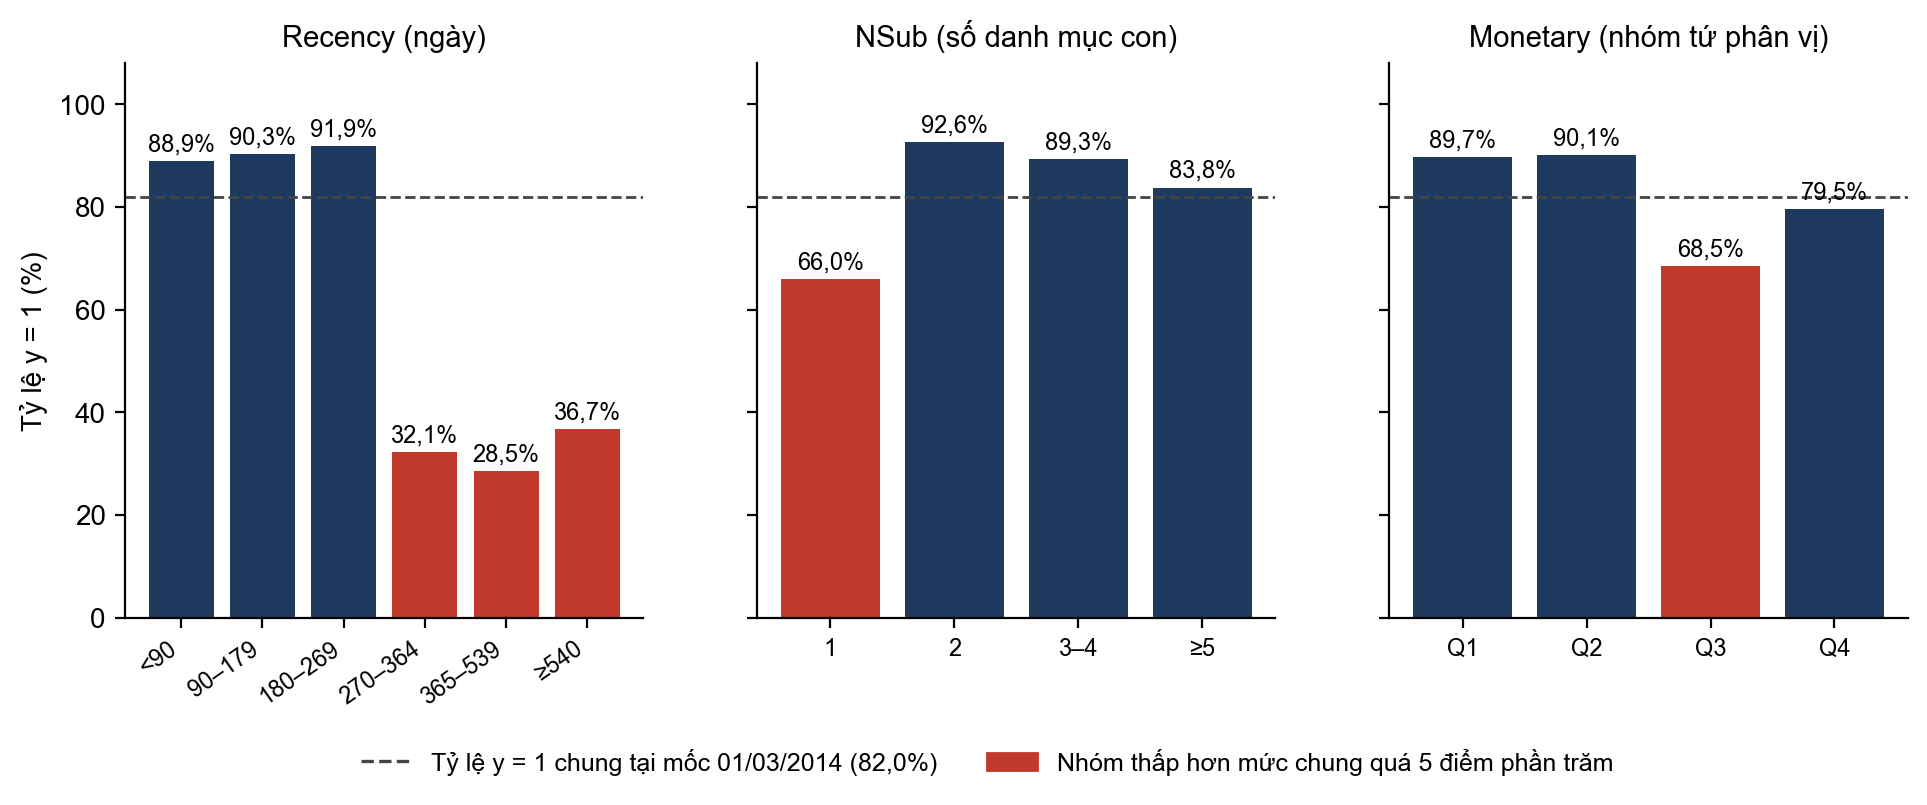
\includegraphics[width=0.7\textwidth]{eda_y_theo_khoang.png}
\caption{Tỷ lệ $y=1$ theo khoảng của Recency, NSub và Monetary}
\label{fig:ytheokhoang}
\end{figure}

\begin{figure}[!tb]
\centering
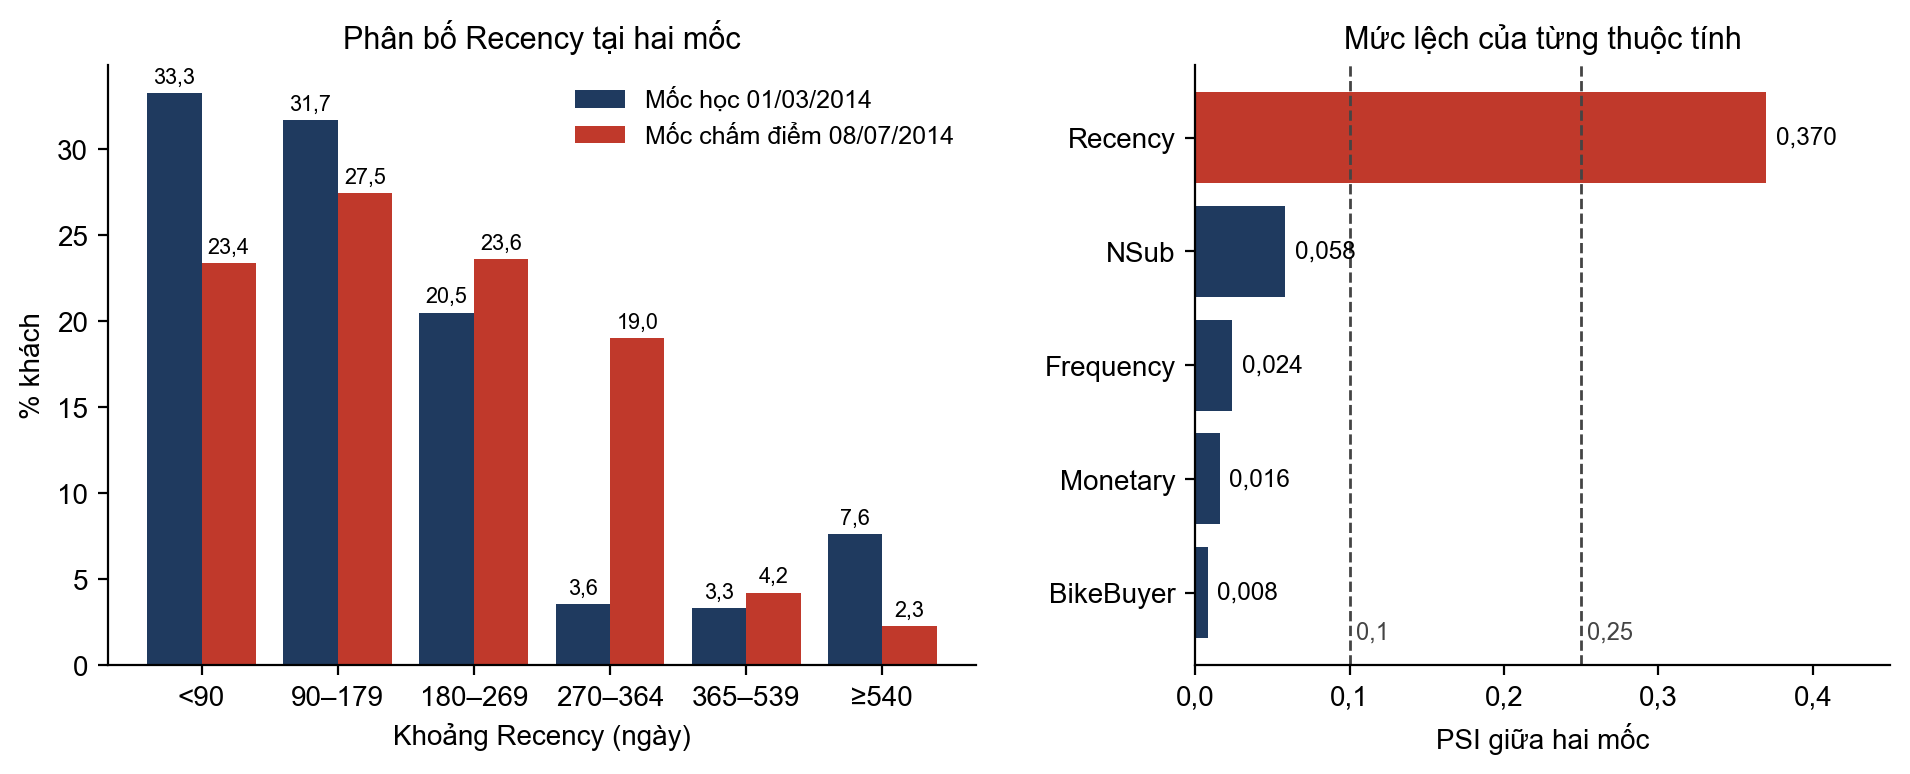
\includegraphics[width=0.42\textwidth]{eda_lech_moc.png}
\caption{Phân bố Recency và PSI của từng thuộc tính giữa mốc huấn luyện và mốc dự đoán}
\label{fig:lechmoc}
\end{figure}

\subsection{Mốc dự đoán có khác mốc huấn luyện không}
Mô hình học tại mốc 01/03/2014 rồi dự đoán tại mốc 08/07/2014, cách nhau 129 ngày, trong khi bốn cặp thử cách nhau 105 đến 106 ngày. Neslin và cộng sự~\cite{neslin2006} ghi nhận trên một cuộc thi dự đoán churn rằng mô hình gần như không giảm độ chính xác khi đem dùng cho dữ liệu thu ba tháng sau tập huấn luyện. Khoảng cách ở đây dài hơn thế, nên nhóm so sánh phân bố giữa hai mốc bằng chỉ số PSI (Population Stability Index, đo mức khác nhau giữa hai phân bố qua các khoảng giá trị, Hình~\ref{fig:lechmoc}), quy ước thường dùng là dưới 0,1 thì hai phân bố giống nhau và trên 0,25 thì khác nhiều.
\begin{itemize}
    \item Recency khác nhiều nhất, PSI là 0,37. Các thuộc tính còn lại đều dưới 0,06.
    \item Khoảng 270 đến 364 ngày chiếm 3,6\% khách ở mốc huấn luyện nhưng 19,0\% ở mốc dự đoán, vì nhóm khách đợt tăng vọt tháng 7/2013 nay rơi vào khoảng này.
    \item Mức khác này không mới: ở bốn cặp thử, PSI của Recency đã là 0,23 đến 0,31.
\end{itemize}
Tuy vậy xác suất của khoảng 270 đến 364 ngày chỉ dựa trên 507 khách của mốc huấn luyện, nên xác suất không mua lại (\texttt{RiskScore}, Chương 5) của nhóm này cần đọc thận trọng.


\textbf{Kiểm tra trước khi huấn luyện.} Nhóm tính lại 10 thuộc tính của 196.985 dòng Snapshot bằng Python, độc lập với SQL, và kết quả khớp hoàn toàn với bảng trong kho. Mười phép kiểm tra miền giá trị đều đạt, ví dụ Tenure không nhỏ hơn Recency và tổng tỷ trọng các nhóm sản phẩm bằng 1.

\clearpage
% Chương Mô hình dự đoán khách hàng rời bỏ
% Bảng m_*.tex và hình m_*.png do python/tao_bang_tex_mohinh.py sinh từ results/. Không sửa tay số liệu trong latex/bang/.
\section{Mô hình dự đoán khách hàng rời bỏ}

Chương này trả lời câu hỏi thứ nhất của đề tài: khách hàng nào có nguy cơ không mua lại. Đầu vào là bảng Customer Snapshot (Chương 3) và nhãn $y$ (Chương 4). Đầu ra là xác suất không mua lại của từng khách, gọi là \texttt{RiskScore}, được ghi vào kho để DSS ở Chương 6 dùng. Chương đi theo quy trình phân lớp hai bước của tài liệu môn học~\cite{tlmh}: học mô hình rồi dùng mô hình để dự đoán. Mọi con số lấy từ kết quả chạy trên kho \texttt{CompanyX\_DW}.

\subsection{Bài toán và tiêu chí chọn mô hình}
\subsubsection{Bài toán}
Đây là bài toán phân lớp hai lớp. Với mỗi khách tại mốc $T$, mô hình nhận các thuộc tính ở Bảng~\ref{tab:thuoctinh} và trả về xác suất $p$ của việc khách không mua lại trong 90 ngày tới ($y=1$). Nhóm cần xác suất chứ không chỉ cần nhãn, vì Chương 6 phải so lợi ích kỳ vọng của việc chăm sóc với chi phí bỏ ra. Hai khách cùng bị dự đoán không mua lại nhưng có xác suất 0,95 và 0,60 thì đáng đầu tư khác nhau.

\subsubsection{Giá trị ròng $Z$: tiêu chí kinh doanh}
Độ chính xác chưa cho biết mô hình có giúp giữ được tiền hay không. Vì vậy nhóm đo thêm giá trị ròng $Z$: số tiền kỳ vọng giữ lại được khi dùng điểm của mô hình để chọn khách chăm sóc trong một ngân sách cố định. Cách tính theo Chương 6: lợi nhuận gộp một đơn của khách $i$ là $v_i = g \cdot AOV_i$, với $AOV_i$ là tiền hàng trung bình mỗi đơn và $g = 41{,}15\%$ là tỷ lệ lợi nhuận gộp tính từ giá vốn. Giá trị kỳ vọng khi chăm sóc khách $i$ là
\begin{equation}
    EV_i = p_i \cdot r \cdot v_i - c
\end{equation}
với $r$ là tỷ lệ chăm sóc thành công và $c$ là chi phí chăm sóc một khách. Danh sách chọn gồm $K = \min(\lfloor B/c \rfloor,\ \text{số khách có } EV_i > 0)$ khách có $p_i v_i$ lớn nhất, với $B$ là ngân sách. Trên mốc đánh giá đã biết nhãn thật $y_i$, giá trị ròng là
\begin{equation}
    Z = r \sum_{i \in S} y_i v_i - c\,K
\end{equation}
với $S$ là danh sách đã chọn. Chỉ khách thật sự không mua lại đem lại lợi ích, vì khách vốn sẽ mua lại thì không cần chăm sóc.

Kịch bản cơ sở là $r = 10\%$, $c = 10$ USD và $B = 40.000$ USD, nên $K = 4.000$. Vì $r$ là giả định, $Z$ chỉ dùng để so các mô hình với nhau, không phải dự báo doanh thu. Hai mốc tham chiếu là chọn chỉ theo giá trị $v$ mà không dùng mô hình (trung bình bốn fold 269.043 USD) và chọn khi biết trước ai không mua lại (346.378 USD). Mô hình hữu ích phải nằm giữa hai mốc này, càng gần mốc sau càng tốt.

\subsubsection{Ba điều kiện chọn mô hình}\label{sec:chon}
Nhóm đặt trước ba điều kiện, mỗi điều kiện ứng với một cách nhìn về mô hình. Một mô hình chỉ được chọn khi đạt cả ba ở mọi fold.
\begin{enumerate}
    \item \textbf{ĐK1, xếp hạng:} ROC-AUC không thấp hơn quy tắc Recency đảo chiều. Cụ thể, khoảng tin cậy 95\% của hiệu hai ROC-AUC (bootstrap, tức lấy mẫu lại có hoàn lại 500 lần để ước lượng khoảng tin cậy~\cite{efron1993}) có cận trên không âm. ROC-AUC và Brier định nghĩa ở mục~\ref{sec:chisobosung}.
    \item \textbf{ĐK2, chất lượng xác suất:} Brier thấp hơn Brier của cách gán cùng một xác suất cho mọi khách.
    \item \textbf{ĐK3, giá trị quyết định:} $Z$ cao hơn $Z$ khi chỉ chọn theo giá trị $v$.
\end{enumerate}
Khi nhiều mô hình cùng đạt, nhóm chọn mô hình có $Z$ cao hơn ở nhiều mốc hơn.

\subsubsection{Các mô hình thử nghiệm}
Nhóm thử chín phương án với cấu hình cố định trước khi chạy (Bảng~\ref{tab:cacmohinh}). Naive Bayes và cây quyết định thuộc nội dung môn học~\cite{han2011}, cây dùng chỉ số Gini của CART~\cite{hastie2009}. Mạng nơ-ron (mục 2.3), Random Forest~\cite{breiman2001}, gradient boosting và kNN~\cite{hastie2009} ngoài nội dung môn học, được thử để biết giới hạn của dữ liệu. Hồi quy logistic và hai mốc so sánh cho biết mô hình chính hơn các cách đơn giản bao nhiêu.

\begin{table}[!htbp]
\centering
\caption{Các mô hình thử nghiệm và cấu hình cố định}
\label{tab:cacmohinh}
\footnotesize
\begin{tabular}{p{3.2cm}p{2.6cm}p{8.6cm}}
\toprule
Mô hình & Vai trò & Cấu hình \\
\midrule
Naive Bayes & Chấm điểm & Năm thuộc tính đã chia khoảng (Recency 6 khoảng, Frequency 3, Monetary 4 theo tứ phân vị, BikeBuyer 2, NSub 4), làm trơn Laplace với hệ số 1 \\
Cây quyết định Gini & Đối chứng, sinh luật & 11 thuộc tính, sâu tối đa 4, mỗi lá có ít nhất 400 khách, xác suất lá làm trơn với $m=50$ \\
Mạng nơ-ron MLP & So sánh & 11 thuộc tính chuẩn hoá z-score, hai tầng ẩn 32 và 16 nơ-ron, ReLU, dừng sớm, hạt giống 0 \\
Hồi quy logistic & So sánh & Năm thuộc tính đã chia khoảng, mã hoá one-hot (mỗi khoảng thành một cột 0/1), chính quy hoá L2 \\
Luôn dự đoán lớp đa số & Mốc so sánh & Xác suất hằng bằng tỷ lệ $y=1$ của mốc huấn luyện \\
Recency đảo chiều & Mốc so sánh & Điểm là thứ hạng phần trăm của Recency, chỉ cho thứ hạng nên không phải xác suất \\
Random Forest, gradient boosting, kNN & Ngoài nội dung môn học & Random Forest 300 cây, gradient boosting độ sâu 4, kNN với $k=200$, đều dùng 11 thuộc tính \\
\bottomrule
\end{tabular}
\end{table}

Xác suất của lá cây được làm trơn bằng ước lượng $m$ để lá nhỏ không cho xác suất cực đoan (ngoài nội dung môn học):
\begin{equation}
    p_{\text{lá}} = \frac{n_{l,1} + m\,\pi}{n_l + m}
\end{equation}
với $n_l$ là số khách trong lá, $n_{l,1}$ là số khách $y=1$ trong lá và $\pi$ là tỷ lệ $y=1$ chung của mốc huấn luyện.

\subsection{Huấn luyện mô hình}
\subsubsection{Giao thức}
Mỗi mô hình được huấn luyện bằng scikit-learn~\cite{pedregosa2011} theo lịch bốn fold ở Bảng~\ref{tab:fold}. Với mỗi cặp $(E \leftarrow T)$, mô hình học trên toàn bộ khách của mốc $T$ rồi chấm điểm toàn bộ khách của mốc $E$. Mọi tham số chia khoảng hay chuẩn hoá chỉ tính trên mốc $T$, để mô hình không nhìn thấy dữ liệu của mốc đánh giá. Toàn bộ vòng huấn luyện và so sánh chạy trong 46 giây trên máy cá nhân. Mô hình chấm điểm thật được học lại trên mốc 01/03/2014 (14.167 khách, tỷ lệ $y=1$ là 82,0\%) rồi chấm 18.360 khách tại mốc 08/07/2014. Mô hình được học lại ở mỗi lần chấm điểm vì cơ cấu khách thay đổi nhanh giữa các mốc (mục~\ref{sec:cauhinh}).

\subsubsection{Chọn tập thuộc tính cho Naive Bayes}
Naive Bayes giả định các thuộc tính độc lập khi đã biết lớp, nên hai thuộc tính nói cùng một điều sẽ bị đếm hai lần. Hệ số tương quan Spearman trên năm mốc huấn luyện cho tám cặp liên quan chặt ($|\rho| \geq 0{,}7$), ví dụ Recency với Orders90 ($-0{,}85$) và Share\_Bikes với BikeBuyer ($0{,}87$). Vì vậy Naive Bayes chỉ dùng năm thuộc tính Recency, Frequency, Monetary, BikeBuyer và NSub. Trong năm thuộc tính này, cặp Monetary và BikeBuyer vẫn phụ thuộc mạnh sau khi chia khoảng (Cramér $V = 0{,}923$), điều này ảnh hưởng đến cách đọc bảng xác suất ở mục~\ref{sec:giaithich}.

Bảng~\ref{tab:tapthuoctinh} so tập thuộc tính thiết kế với các tập khác theo cùng giao thức. NSub có ích: bỏ NSub làm ROC-AUC giảm từ 0,720 xuống 0,701, Brier tăng từ 0,125 lên 0,133, $Z$ giảm 2.577 USD và không fold nào còn đạt ĐK1. Bỏ BikeBuyer, Frequency hoặc Monetary chỉ đổi $Z$ dưới 1\%, nhỏ hơn mức dao động giữa các fold. Thêm Tenure hay Orders180 làm ROC-AUC tăng nhưng Brier xấu đi và $Z$ giảm 8.093 và 11.215 USD, đúng với tương quan mạnh của hai thuộc tính này với Monetary và Recency. Nhóm giữ tập thiết kế vì quy tắc chọn đã chốt từ trước và để tránh chọn lại cấu hình trên chính bốn fold dùng để phát triển. Đây là một đánh đổi: bỏ BikeBuyer cho ROC-AUC 0,729 cao hơn nhưng $Z$ thấp hơn 830 USD.

\begin{table}[!htbp]
\centering
\caption{Naive Bayes theo tập thuộc tính, trung bình bốn fold}
\label{tab:tapthuoctinh}
\footnotesize
\resizebox{\textwidth}{!}{\begin{tabular}{lrrrrcc}
\toprule
Tập thuộc tính & ROC-AUC & Brier & $Z$ (USD) & Chênh $Z$ & Số fold $Z$ cao hơn & ĐK1 \\
\midrule
Thiết kế: R, F, M, BikeBuyer, NSub & 0,720 & 0,125 & 291.883 & -- & -- & 4/4 \\
Bỏ NSub & 0,701 & 0,133 & 289.306 & $-$2.577 & 0/4 & 0/4 \\
Bỏ BikeBuyer & 0,729 & 0,124 & 291.053 & $-$830 & 1/4 & 4/4 \\
Bỏ Frequency & 0,725 & 0,124 & 291.340 & $-$543 & 2/4 & 4/4 \\
Bỏ Monetary & 0,722 & 0,123 & 289.869 & $-$2.014 & 2/4 & 4/4 \\
Chỉ R, F, M & 0,708 & 0,131 & 287.457 & $-$4.426 & 0/4 & 2/4 \\
Thêm Tenure & 0,732 & 0,131 & 283.791 & $-$8.093 & 1/4 & 4/4 \\
Thêm Orders180 & 0,727 & 0,137 & 280.668 & $-$11.215 & 0/4 & 4/4 \\
\bottomrule
\end{tabular}
}
\end{table}

\subsubsection{So sánh các cấu hình}\label{sec:cauhinh}
Bảng~\ref{tab:cauhinh} cho kết quả khi đổi cách học hoặc cấu hình. Học lại ở mốc gần nhất tốt hơn: Naive Bayes học tại mốc gần nhất cho $Z = 291.883$ USD, cao hơn học một lần ở mốc đầu (283.465 USD) và gộp mọi mốc (281.033 USD), khớp với nhận xét ở Chương 4 rằng cơ cấu khách đổi rõ giữa các mốc. Cây ít nhạy với cấu hình: độ sâu từ 3 đến 6 và số khách tối thiểu mỗi lá từ 200 đến 800 chỉ làm ROC-AUC dao động từ 0,669 đến 0,687, còn $m$ từ 0 đến 200 gần như không đổi kết quả, nên nhóm giữ cấu hình xuất phát vì cho luật ngắn nhất. Với mạng nơ-ron, kiến trúc (32, 16) tốt hơn (16) và (64, 32).

\begin{table}[!htbp]
\centering
\caption{So sánh cấu hình, trung bình bốn fold}
\label{tab:cauhinh}
\footnotesize
\begin{tabular}{lrrr}
\toprule
Cấu hình & ROC-AUC & Brier & $Z$ (USD) \\
\midrule
Naive Bayes, học tại mốc gần nhất (thiết kế) & 0,720 & 0,125 & 291.883 \\
Naive Bayes, học một lần ở mốc đầu & 0,717 & 0,131 & 283.465 \\
Naive Bayes, gộp mọi mốc đủ nhãn & 0,713 & 0,134 & 281.033 \\
Cây sâu 3 & 0,669 & 0,140 & 282.077 \\
Cây sâu 4 (thiết kế) & 0,680 & 0,140 & 281.490 \\
Cây sâu 5 & 0,683 & 0,140 & 280.941 \\
Cây sâu 6 & 0,687 & 0,139 & 281.633 \\
Cây, 200 khách mỗi lá & 0,676 & 0,143 & 280.081 \\
Cây, 800 khách mỗi lá & 0,671 & 0,141 & 278.360 \\
Cây, $m=0$ & 0,683 & 0,140 & 281.636 \\
Cây, $m=200$ & 0,680 & 0,139 & 281.314 \\
MLP (16) & 0,708 & 0,140 & 284.725 \\
MLP (32, 16) & 0,751 & 0,128 & 288.379 \\
MLP (64, 32) & 0,741 & 0,128 & 287.443 \\
\bottomrule
\end{tabular}

\end{table}

\subsection{Kết quả và chọn mô hình}
\subsubsection{Kết quả trung bình bốn fold}
Bảng~\ref{tab:trungbinh} và Hình~\ref{fig:zmohinh} tổng hợp kết quả. Chỉ Naive Bayes, mạng nơ-ron, gradient boosting và kNN đạt cả ba điều kiện ở 4/4 fold. Trong bốn mô hình này Naive Bayes có Brier thấp nhất (0,125) và $Z$ cao nhất (291.883 USD).

\begin{table}[!htbp]
\centering
\caption{Kết quả trung bình bốn fold và số fold đạt từng điều kiện}
\label{tab:trungbinh}
\footnotesize
\begin{tabular}{lrrrccc}
\toprule
Mô hình & ROC-AUC & Brier & $Z$ (USD) & ĐK1 & ĐK2 & ĐK3 \\
\midrule
Naive Bayes rời rạc & 0,720 & 0,125 & 291.883 & 4/4 & 4/4 & 4/4 \\
Mạng nơ-ron MLP (32, 16) & 0,751 & 0,128 & 288.379 & 4/4 & 4/4 & 4/4 \\
Cây Gini (sâu 4, 400 khách mỗi lá) & 0,680 & 0,140 & 281.490 & 1/4 & 3/4 & 4/4 \\
Hồi quy logistic & 0,659 & 0,151 & 273.406 & 1/4 & 2/4 & 2/4 \\
Recency đảo chiều & 0,717 & 0,269 & 253.315 & 4/4 & 0/4 & 1/4 \\
Luôn dự đoán lớp đa số & 0,500 & 0,149 & 269.043 & 0/4 & 0/4 & 0/4 \\
Random Forest (300 cây) & 0,724 & 0,131 & 288.179 & 3/4 & 4/4 & 4/4 \\
Gradient boosting & 0,741 & 0,131 & 283.224 & 4/4 & 4/4 & 4/4 \\
kNN ($k=200$) & 0,741 & 0,131 & 283.557 & 4/4 & 4/4 & 4/4 \\
\bottomrule
\end{tabular}

\end{table}

\begin{figure}[!htbp]
\centering
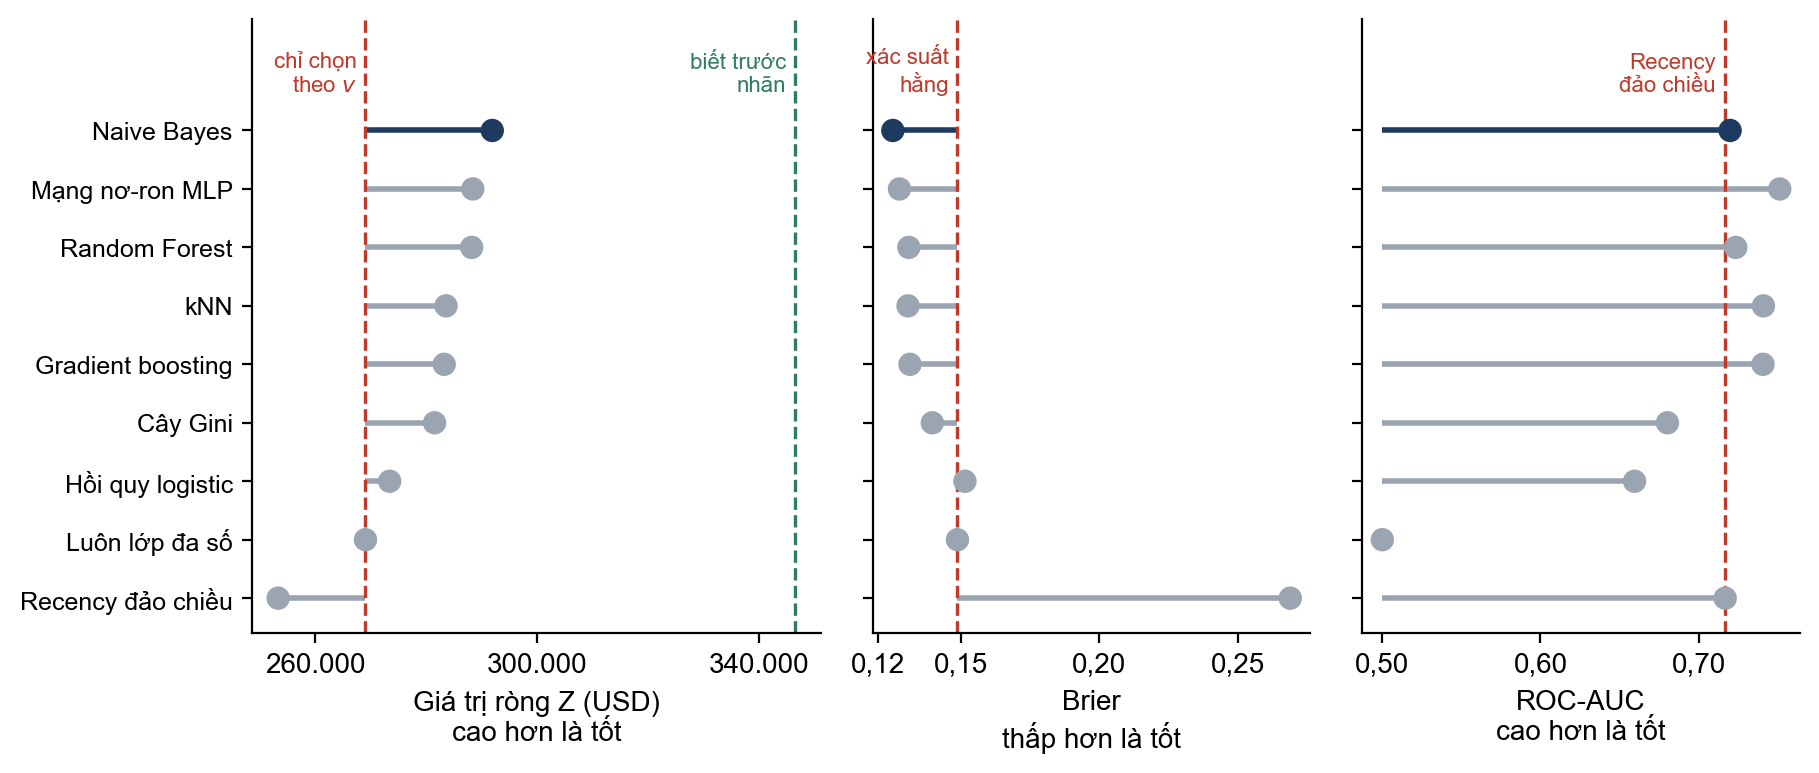
\includegraphics[width=0.95\textwidth]{m_z_mo_hinh.png}
\caption{Ba tiêu chí của chín phương án, trung bình bốn fold}
\label{fig:zmohinh}
\end{figure}

Mạng nơ-ron xếp hạng tốt nhất (ROC-AUC 0,751 so với 0,720), nhưng Naive Bayes có $Z$ cao hơn ở cả bốn mốc, chênh trung bình 3.504 USD, tức 1,2\% (Bảng~\ref{tab:nbmlp}). Theo luật chọn, Naive Bayes thắng. Mạng nơ-ron còn đổi kết quả theo hạt giống khởi tạo: ROC-AUC tại mốc 15/01/2014 dao động từ 0,710 đến 0,769 giữa ba hạt giống, và ở mọi hạt giống $Z$ đều thấp hơn Naive Bayes ở cả bốn mốc (Hình~\ref{fig:nbmlpseed}). Naive Bayes là mô hình xác định, cho cùng kết quả trên mọi máy.

\begin{table}[!htbp]
\centering
\caption{Giá trị ròng $Z$ (USD) của Naive Bayes và mạng nơ-ron tại từng mốc đánh giá}
\label{tab:nbmlp}
\footnotesize
\begin{tabular}{lrrr}
\toprule
Mốc đánh giá $E$ & $Z$ Naive Bayes & $Z$ MLP & Chênh lệch \\
\midrule
15/12/2013 & 292.046 & 290.319 & 1.727 \\
15/01/2014 & 293.085 & 290.012 & 3.073 \\
15/02/2014 & 293.156 & 289.820 & 3.336 \\
01/03/2014 & 289.246 & 283.366 & 5.880 \\
Trung bình & 291.883 & 288.379 & 3.504 \\
\bottomrule
\end{tabular}

\end{table}

\begin{figure}[!htbp]
\centering
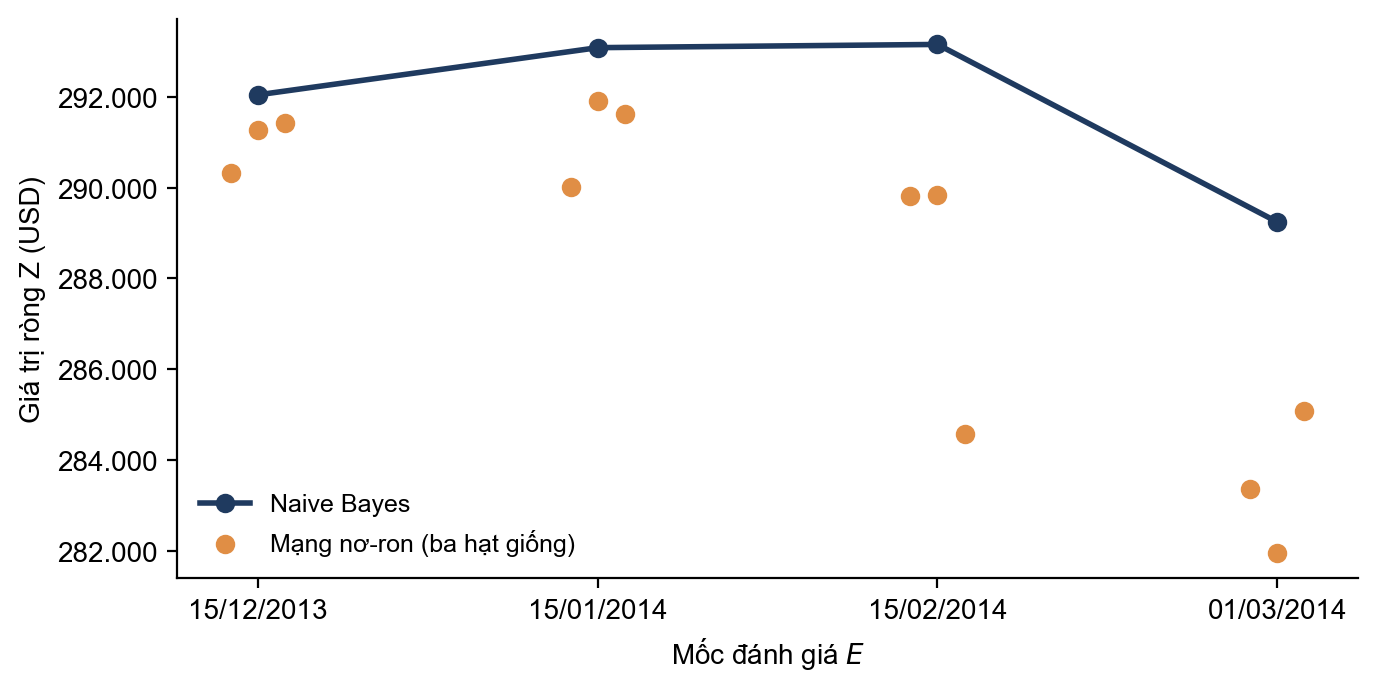
\includegraphics[width=0.7\textwidth]{m_nb_mlp_seed.png}
\caption{Giá trị ròng $Z$ của Naive Bayes và mạng nơ-ron với ba hạt giống}
\label{fig:nbmlpseed}
\end{figure}

Quy tắc Recency đảo chiều xếp hạng gần bằng Naive Bayes (0,717 so với 0,720) nhưng Brier tới 0,269, nên không đạt ĐK2 ở fold nào. Hồi quy logistic có ROC-AUC 0,659, thấp hơn cả quy tắc Recency. Random Forest, gradient boosting và kNN xếp hạng tốt hơn Naive Bayes (ROC-AUC từ 0,724 đến 0,741) nhưng $Z$ không cao hơn. Với bài toán này, xác suất sát thực tế quan trọng hơn khả năng xếp hạng.

\subsubsection{Cây đối chứng: vì sao không dùng để chấm điểm}
Cây Gini đạt điều kiện về $Z$ ở 4/4 fold nhưng ROC-AUC chỉ 0,680 và thấp hơn quy tắc Recency ở 3/4 fold. Nguyên nhân là cây chỉ có 9 đến 11 lá, nên xác suất thô và nhóm nhỏ không tách được thành lá riêng. Vì vậy cây không chấm điểm mà sinh luật IF--THEN để mô tả nhóm khách (mục~\ref{sec:giaithich}). Nút gốc luôn là Recency với ngưỡng từ 131,5 đến 170,5 ngày ở cả bốn mốc, nên luật nhất quán giữa các kỳ.

\subsubsection{Xem kỹ Naive Bayes tại fold cuối}
Phần này xem kỹ Naive Bayes ở fold cuối ($E = 01/03/2014$, học tại $T = 15/11/2013$). Bảng~\ref{tab:lop1} và Hình~\ref{fig:matran} cho ma trận nhầm lẫn và các chỉ số của môn học~\cite{han2011} ở ba cách đặt ngưỡng, cùng cách luôn dự đoán $y=1$ để làm mốc. Ngưỡng Youden~\cite{youden1950} là ngưỡng làm tổng sensitivity (tức recall ở Chương 2) và specificity lớn nhất.

\begin{table}[!htbp]
\centering
\caption{Ma trận nhầm lẫn và chỉ số phân lớp của Naive Bayes tại mốc 01/03/2014}
\label{tab:lop1}
\footnotesize
\resizebox{\textwidth}{!}{\begin{tabular}{lrrrr}
\toprule
Chỉ số & Youden, mốc huấn luyện & Youden, ngoài mẫu & Mức Cao của DSS & Luôn $y=1$ \\
\midrule
Số khách dự đoán $y=1$ & 11.650 & 9.125 & 3.544 & 14.167 \\
Tỷ lệ khách dự đoán $y=1$ & 82,2\% & 64,4\% & 25,0\% & 100,0\% \\
TP & 10.477 & 8.171 & 3.182 & 11.612 \\
FN & 1.135 & 3.441 & 8.430 & 0 \\
FP & 1.173 & 954 & 362 & 2.555 \\
TN & 1.382 & 1.601 & 2.193 & 0 \\
Accuracy & 0,837 & 0,690 & 0,379 & 0,820 \\
Tỷ lệ lỗi (error rate) & 0,163 & 0,310 & 0,621 & 0,180 \\
Precision & 0,899 & 0,895 & 0,898 & 0,820 \\
Sensitivity (recall) & 0,902 & 0,704 & 0,274 & 1,000 \\
Specificity & 0,541 & 0,627 & 0,858 & 0,000 \\
F1 & 0,901 & 0,788 & 0,420 & 0,901 \\
\bottomrule
\end{tabular}
}
\end{table}

\begin{figure}[!htbp]
\centering
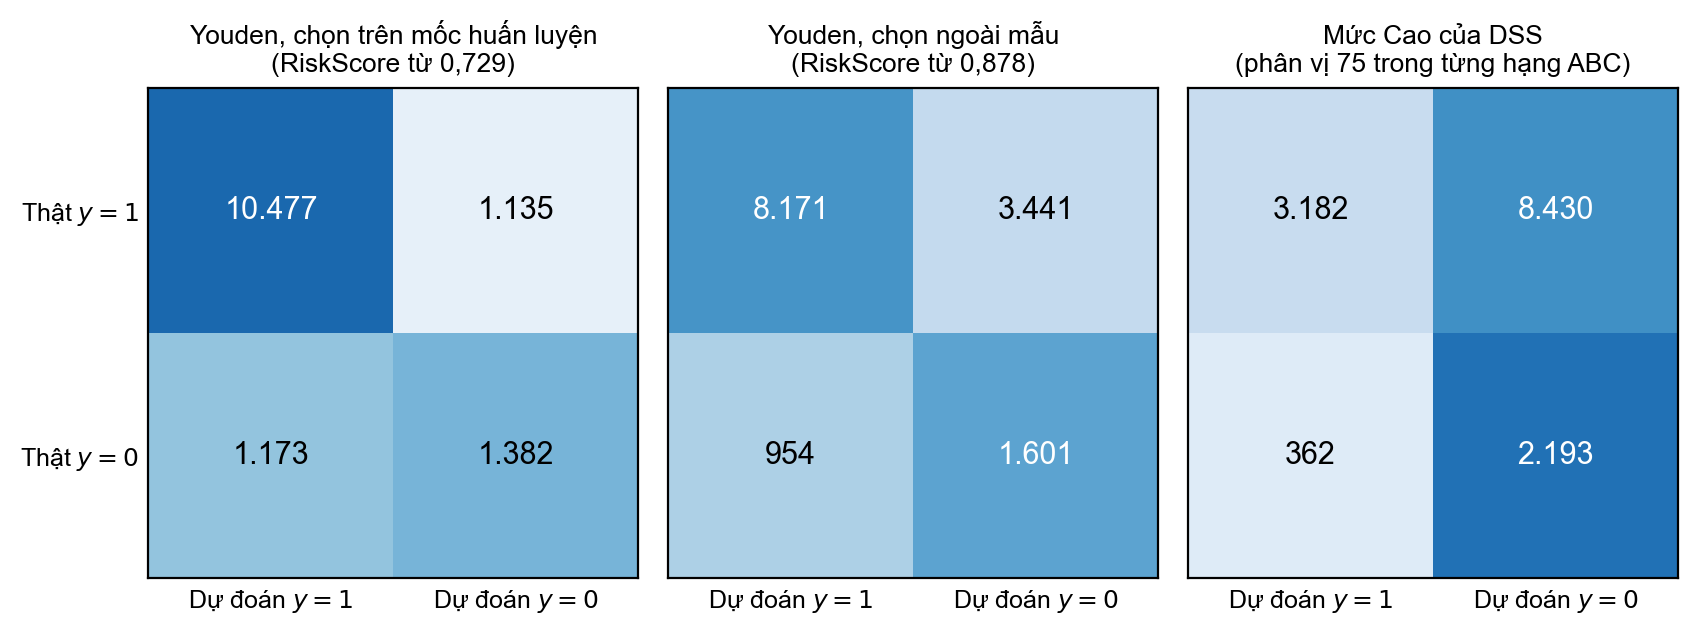
\includegraphics[width=0.95\textwidth]{m_ma_tran.png}
\caption{Ma trận nhầm lẫn của Naive Bayes ở ba cách đặt ngưỡng}
\label{fig:matran}
\end{figure}

Ngưỡng Youden chọn trên mốc huấn luyện cảnh báo 82,2\% số khách, đạt accuracy 0,837 và F1 0,901. Con số đẹp này là do lớp $y=1$ chiếm 82,0\% số khách: cách luôn dự đoán $y=1$ cũng đạt accuracy 0,820 và F1 0,901 nhưng specificity bằng 0. Vì vậy accuracy và F1 không dùng được một mình khi lớp mục tiêu chiếm đa số. Ngưỡng Youden chọn ngoài mẫu (trên mốc 15/11/2013) chỉ cảnh báo 64,4\% khách và cân bằng hơn hẳn (sensitivity 0,704, specificity 0,627), cho thấy ngưỡng chọn trên chính mốc huấn luyện là lạc quan.

Mức Cao của DSS (phân vị 75 trong từng hạng ABC) chỉ cảnh báo 25,0\% khách, nên sensitivity thấp theo chủ ý. Điều quan trọng là precision đạt 0,898 so với tỷ lệ nền 0,820: trong 10 khách mức Cao có khoảng 9 khách thật sự không mua lại, và specificity 0,858 nghĩa là ít khách sẽ mua lại bị làm phiền. Mức Cao là danh sách ưu tiên chứ không phải bộ phát hiện đầy đủ: nó có ít cảnh báo sai nhất (362 khách) nhưng bỏ sót nhiều khách $y=1$ nhất (8.430 khách). Nhóm không gắn mức Cao vẫn có 79,4\% khách $y=1$, chỉ thấp hơn tỷ lệ nền 2,6 điểm phần trăm, nên mô hình tách hai nhóm khách ở mức vừa phải, phù hợp với ROC-AUC 0,72.

Bảng~\ref{tab:lop23} cho hai nhóm chỉ số còn lại: chất lượng xác suất và giá trị quyết định. ROC-AUC của Naive Bayes (0,7207) chỉ nhỉnh hơn Recency đảo chiều (0,7191), đây là điểm yếu cần thừa nhận. Giá trị của mô hình nằm ở xác suất: Brier đạt 0,1176 so với 0,1480 của cách gán xác suất hằng. Khi chọn theo $p \cdot v$, $Z$ đạt 289.245,54 USD, cao hơn 13,7\% so với 254.292,63 USD khi chỉ chọn theo $v$, và lấp được khoảng 41\% khoảng cách từ mức đó đến mức trần 339.886,26 USD khi biết trước nhãn. Nói cách khác, Recency đủ để biết ai có nguy cơ, nhưng cần xác suất tốt để quyết định chi ngân sách cho ai. Hình~\ref{fig:rocpr} vẽ đường ROC (tỷ lệ bắt đúng khách $y=1$ theo tỷ lệ báo nhầm khách $y=0$ khi ngưỡng thay đổi, diện tích dưới đường là ROC-AUC) và cho thấy đường của Naive Bayes và Recency đảo chiều gần trùng nhau, mạng nơ-ron cao hơn ở vùng giữa, còn cây có dạng bậc thang vì chỉ có 11 mức xác suất. Đường Precision--Recall được vẽ thêm vì lớp $y=1$ chiếm khoảng 82\%~\cite{saito2015}.

\begin{table}[!htbp]
\centering
\caption{Chất lượng điểm và giá trị quyết định của Naive Bayes tại mốc 01/03/2014}
\label{tab:lop23}
\footnotesize
\begin{tabular}{llr}
\toprule
Lớp & Chỉ số & Giá trị tại mốc 01/03/2014 \\
\midrule
Xếp hạng & ROC-AUC của Naive Bayes & 0,7207 \\
 & ROC-AUC của Recency đảo chiều & 0,7191 \\
 & Average precision, lớp $y=1$ & 0,893 \\
 & Average precision, lớp $y=0$ & 0,476 \\
 & Precision@4.000 & 89,33\% \\
Chất lượng xác suất & Brier của Naive Bayes & 0,1176 \\
 & Brier của cách dự đoán một xác suất hằng & 0,1480 \\
Giá trị quyết định & $Z$ khi chọn theo $p\cdot v$ (USD) & 289.245,54 \\
 & $Z$ khi chỉ chọn theo $v$ (USD) & 254.292,63 \\
 & $Z$ khi biết trước nhãn (USD) & 339.886,26 \\
\bottomrule
\end{tabular}

\end{table}

\begin{figure}[!htbp]
\centering
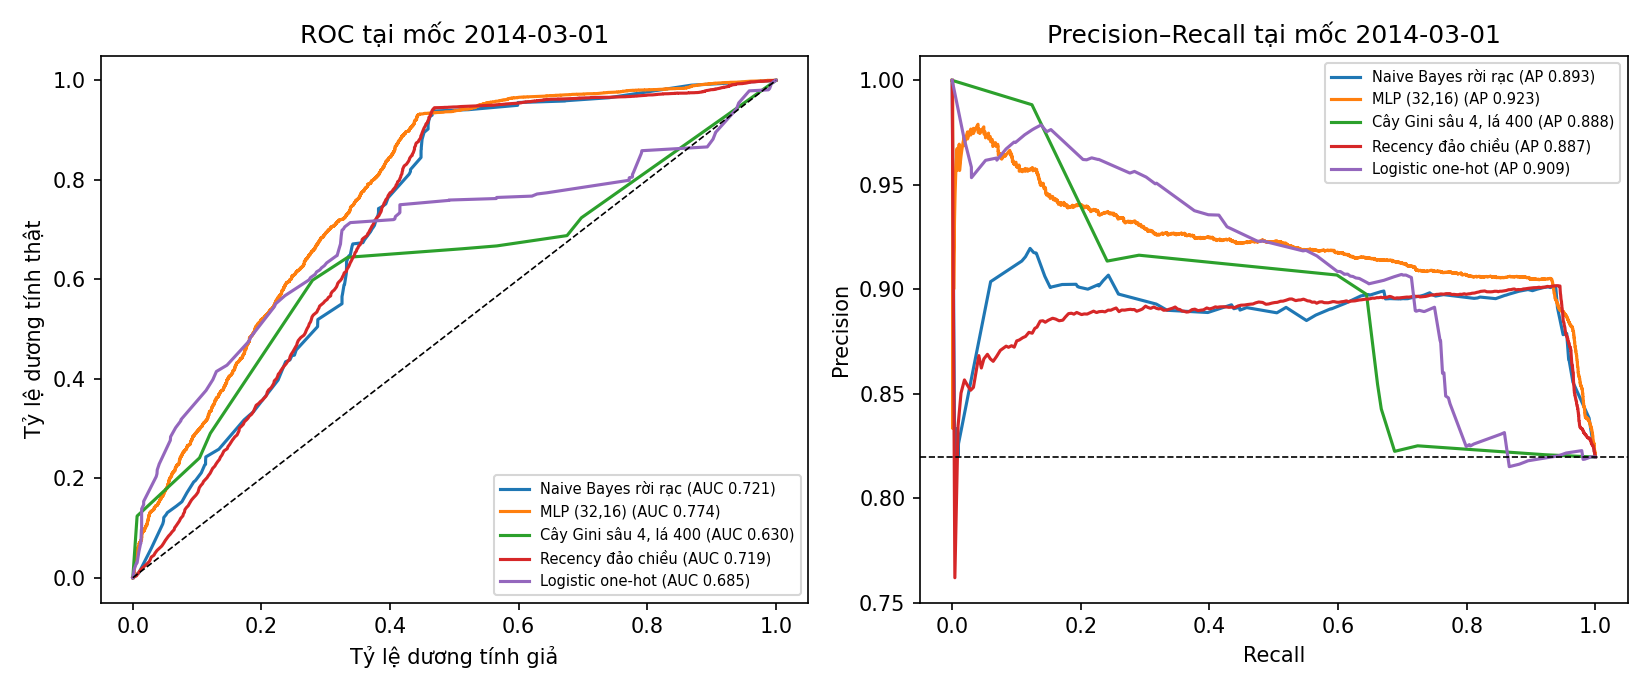
\includegraphics[width=\textwidth]{m_roc_pr.png}
\caption{Đường ROC (trái) và Precision--Recall (phải) tại mốc 01/03/2014}
\label{fig:rocpr}
\end{figure}

\subsubsection{Nhãn 90 ngày và nhãn 180 ngày}\label{sec:nhan180}
Nhãn $y=1$ gồm cả khách đã bỏ đi lẫn khách chưa đến kỳ mua lại. Để đo mức nhiễu này, nhóm so nhãn 90 ngày với nhãn 180 ngày ở 13 mốc từ 01/06/2013 đến 01/12/2013, là các mốc có cửa sổ 180 ngày đã khép (Bảng~\ref{tab:nhan180}). Tỷ lệ $y=1$ trung bình giảm từ 80,8\% xuống 59,6\%. Trong số khách bị gắn $y=1$ theo nhãn 90 ngày, 26,2\% có mua lại trong ngày 90 đến 180, tức khoảng một phần tư là khách chưa đến kỳ chứ chưa bỏ đi. Khi đối chiếu điểm của mô hình học theo nhãn 90 ngày với nhãn 180 ngày ở ba mốc cuối, ROC-AUC trung bình của Naive Bayes tăng từ 0,694 lên 0,752, nghĩa là điểm rủi ro xếp hạng tốt hơn với hành vi không mua lại kéo dài. Quy tắc Recency tăng tương tự (0,693 lên 0,759), cây tăng ít hơn (0,653 lên 0,678).

\begin{table}[!htbp]
\centering
\caption{Tỷ lệ $y=1$ theo nhãn 90 ngày và 180 ngày tại các mốc có đủ cửa sổ 180 ngày}
\label{tab:nhan180}
\footnotesize
\begin{tabular}{lR{1.6cm}R{2.0cm}R{2.0cm}R{3.6cm}R{2.2cm}}
\toprule
Mốc $T$ & Số khách & $y=1$ (90 ngày) & $y=1$ (180 ngày) & Khách $y=1$ mua lại trong ngày 90--180 & Tỷ lệ chưa đến kỳ \\
\midrule
01/06/2013 & 5.324 & 82,8\% & 60,1\% & 1.205 & 27,4\% \\
15/06/2013 & 5.423 & 82,6\% & 59,1\% & 1.271 & 28,4\% \\
01/07/2013 & 5.536 & 82,2\% & 57,5\% & 1.363 & 30,0\% \\
15/07/2013 & 5.889 & 82,0\% & 57,2\% & 1.457 & 30,2\% \\
01/08/2013 & 6.529 & 81,5\% & 57,6\% & 1.563 & 29,4\% \\
15/08/2013 & 7.077 & 80,3\% & 58,3\% & 1.555 & 27,4\% \\
01/09/2013 & 7.705 & 79,5\% & 59,1\% & 1.572 & 25,7\% \\
15/09/2013 & 8.249 & 79,6\% & 59,7\% & 1.640 & 25,0\% \\
01/10/2013 & 8.812 & 79,4\% & 59,9\% & 1.720 & 24,6\% \\
15/10/2013 & 9.305 & 79,3\% & 60,0\% & 1.795 & 24,3\% \\
01/11/2013 & 9.898 & 79,4\% & 60,8\% & 1.835 & 23,4\% \\
15/11/2013 & 10.447 & 80,7\% & 62,5\% & 1.899 & 22,5\% \\
01/12/2013 & 11.055 & 81,4\% & 63,4\% & 1.986 & 22,1\% \\
\bottomrule
\end{tabular}

\end{table}

Nhóm không huấn luyện thẳng một mô hình với nhãn 180 ngày, vì khi đó mốc huấn luyện phải trước 01/06/2013, mà tại đó mọi khách chỉ có một đơn, đều đã mua xe đạp và có $NSub = 1$ nên không có gì để học. Vì vậy nhãn 90 ngày được giữ, và \texttt{RiskScore} cần hiểu là khả năng không mua lại trong kỳ tới, không phải xác suất khách đã rời bỏ hẳn.

\subsubsection{Kết luận chọn mô hình và giới hạn}
Naive Bayes là mô hình chấm điểm vì đạt cả ba điều kiện ở 4/4 fold và có $Z$ cao hơn mạng nơ-ron ở 4/4 mốc. Cây Gini giữ vai trò đối chứng và sinh luật, mạng nơ-ron chỉ để so sánh. Có ba giới hạn cần nhớ. Bốn fold có cửa sổ nhãn chồng nhau và cấu hình cũng được chọn trên chính bốn fold này, nên kết quả có thiên lệch lựa chọn. Chênh lệch $Z$ giữa Naive Bayes và mạng nơ-ron (1,2\%) nhỏ hơn mức dao động của mạng nơ-ron giữa các hạt giống, nên Naive Bayes được chọn vì thắng nhất quán ở mọi mốc và mọi hạt giống, không vì độ lớn của chênh lệch. Khả năng xếp hạng chỉ ngang quy tắc Recency, nên lợi thế của mô hình đến từ chất lượng xác suất.

\subsection{Giải thích dự đoán}\label{sec:giaithich}
Người ra quyết định cần biết vì sao một khách bị chấm điểm cao. Nhóm giải thích ở hai tầng: tầng một cho biết thuộc tính nào kéo xác suất lên hay xuống, tầng hai mô tả khách thuộc nhóm nào.

\subsubsection{Tầng một: xác suất có điều kiện của Naive Bayes}
Bảng~\ref{tab:xacsuat} và Hình~\ref{fig:tysonb} cho xác suất của từng giá trị thuộc tính trong mỗi lớp, ước lượng trên mốc 01/03/2014. Tỷ số $P(x \mid y=1)/P(x \mid y=0)$ lớn hơn 1 nghĩa là giá trị đó làm tăng rủi ro. Recency chi phối: Recency từ 180 đến 269 ngày có tỷ số 2,495, tăng rủi ro mạnh nhất, còn Recency từ 270 đến 539 ngày có tỷ số 0,09 đến 0,10, giảm rủi ro rất mạnh. Điều này khớp với Hình~\ref{fig:ytheokhoang}: nhóm sau chủ yếu là khách của đợt tăng vọt tháng 7/2013 nay đã đến kỳ mua lại. Monetary thấp (Q1) có tỷ số 1,907, NSub bằng 2 có 2,748. Hai thuộc tính Monetary và BikeBuyer phụ thuộc mạnh nên Naive Bayes đếm hai lần cùng thông tin ``đã mua xe đắt'', không cộng dồn hai dòng này khi diễn giải. Trong cây đối chứng, độ quan trọng Gini của Recency là 0,83 và của Monetary là 0,12, còn NSub bằng 0 vì cây sâu 4 đã dùng hết các phép tách cho hai thuộc tính trước. Giá trị của NSub chỉ thể hiện qua Naive Bayes (Bảng~\ref{tab:tapthuoctinh}).

\begin{table}[!htbp]
\centering
\caption{Xác suất có điều kiện của Naive Bayes tại mốc huấn luyện 01/03/2014}
\label{tab:xacsuat}
\footnotesize
\begin{tabular}{llrrr}
\toprule
Thuộc tính & Khoảng & $P(x\mid y=0)$ & $P(x\mid y=1)$ & Tỷ số \\
\midrule
Recency & $<$90 & 20,4\% & 36,1\% & 1,77 \\
 & 90--179 & 17,0\% & 34,9\% & 2,06 \\
 & 180--269 & 9,2\% & 23,0\% & 2,50 \\
 & 270--364 & 13,5\% & 1,4\% & 0,10 \\
 & 365--539 & 13,2\% & 1,2\% & 0,09 \\
 & $\geq$540 & 26,8\% & 3,4\% & 0,13 \\
Frequency & 1 & 75,8\% & 67,9\% & 0,90 \\
 & 2 & 19,9\% & 27,5\% & 1,38 \\
 & $\geq$3 & 4,2\% & 4,6\% & 1,09 \\
Monetary & Q1 (thấp nhất) & 14,4\% & 27,5\% & 1,91 \\
 & Q2 & 13,6\% & 27,4\% & 2,01 \\
 & Q3 & 43,6\% & 20,9\% & 0,48 \\
 & Q4 (cao nhất) & 28,3\% & 24,2\% & 0,85 \\
BikeBuyer & 0 & 28,8\% & 49,7\% & 1,73 \\
 & 1 & 71,2\% & 50,3\% & 0,71 \\
NSub & 1 & 66,0\% & 28,2\% & 0,43 \\
 & 2 & 13,4\% & 36,7\% & 2,75 \\
 & 3--4 & 16,6\% & 30,6\% & 1,84 \\
 & $\geq$5 & 4,0\% & 4,5\% & 1,13 \\
\bottomrule
\end{tabular}

\end{table}

\begin{figure}[!htbp]
\centering
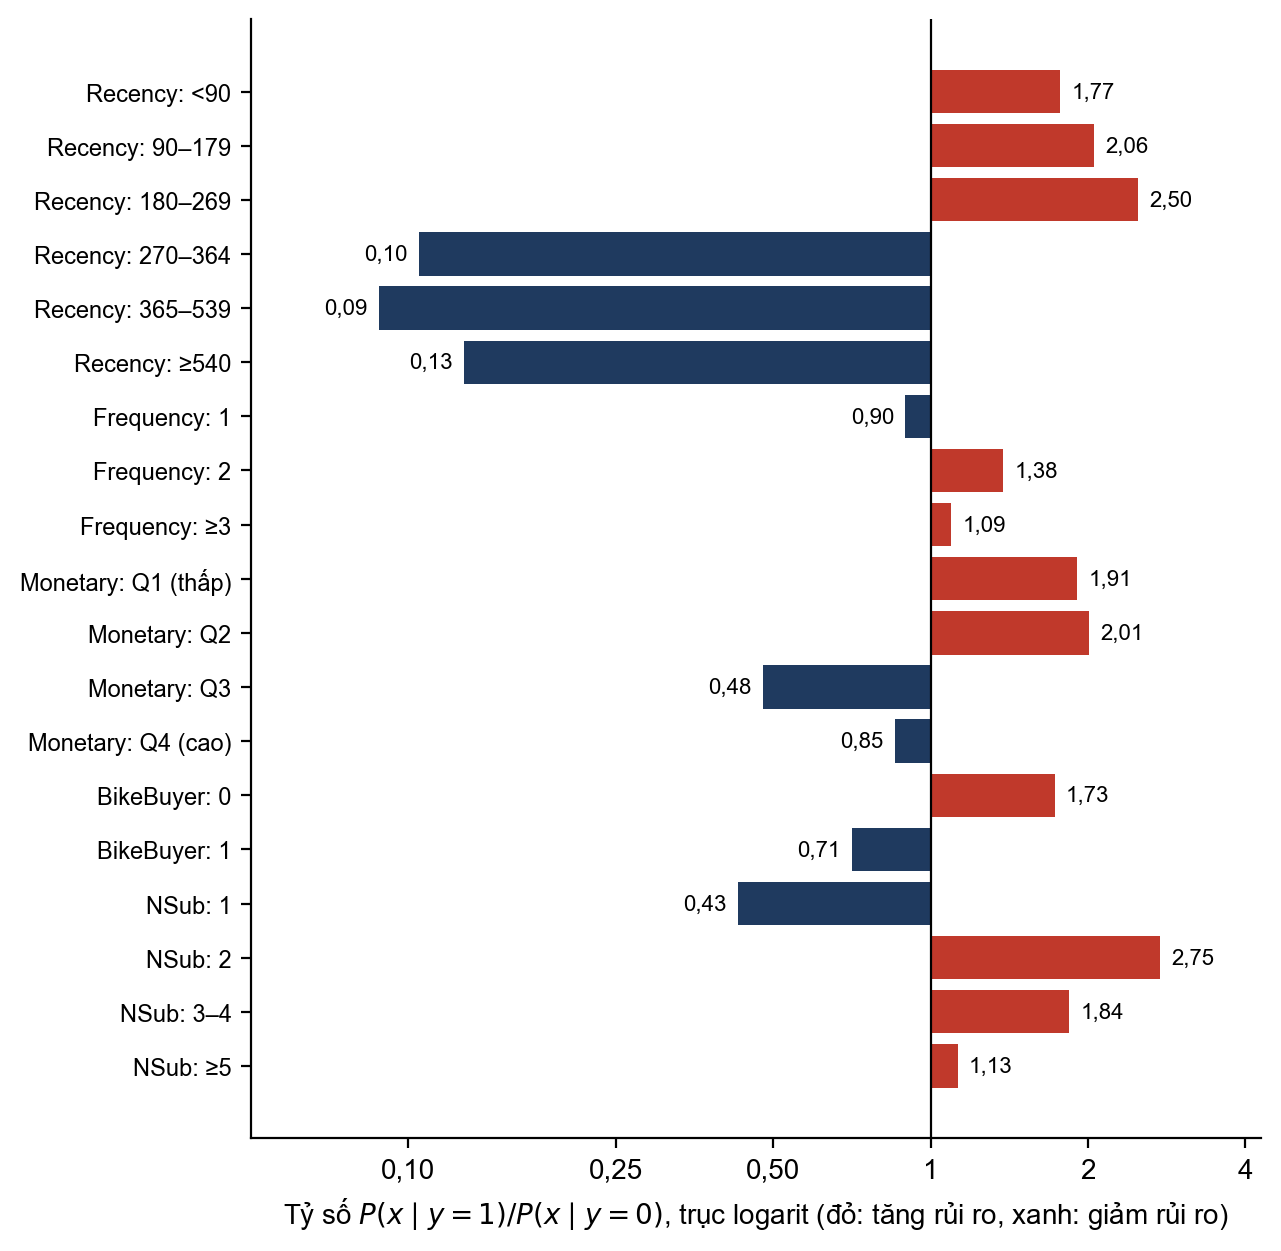
\includegraphics[width=0.62\textwidth]{m_ty_so_nb.png}
\caption{Tỷ số xác suất có điều kiện của Naive Bayes theo khoảng thuộc tính}
\label{fig:tysonb}
\end{figure}

\subsubsection{Tầng hai: luật của cây đối chứng}
Cây học trên mốc 01/03/2014 có 11 lá (Bảng~\ref{tab:lacay}), trong đó 6 lá có tỷ lệ $y=1$ thấp hơn tỷ lệ chung 82,0\%. Mỗi lá là một luật mô tả một nhóm khách giống nhau, kèm tỷ lệ $y=1$ của nhóm và \texttt{TreeScore}, là xác suất của lá sau làm trơn. Đây là mô tả nhóm, không phải lý do tính ra \texttt{RiskScore}. Nhóm có tỷ lệ $y=1$ thấp nhất là lá 8 (Recency trên 275,5 ngày, Tenure không quá 744 ngày, Monetary không quá 1.684,87 USD) với 18,1\%: khách đã lâu không mua nhưng hầu hết vẫn quay lại. DSS hiển thị luật thành câu tiếng Việt, ví dụ ``lần mua gần nhất cách đây trên 275 ngày, đã là khách không quá 744 ngày''.

\begin{table}[!htbp]
\centering
\caption{Các lá của cây đối chứng học tại mốc 01/03/2014 (14.167 khách)}
\label{tab:lacay}
\footnotesize
\begin{tabular}{cp{8.6cm}rrr}
\toprule
Lá & Luật (IF) & Số khách & $y=1$ thô & TreeScore \\
\midrule
1 & Recency $\leq$ 275,5, Monetary $\leq$ 4.640,88, chưa mua xe đạp, Monetary $\leq$ 150,94 & 6.054 & 89,9\% & 0,898 \\
2 & Recency $\leq$ 275,5, Monetary $\leq$ 4.640,88, chưa mua xe đạp, Monetary $>$ 150,94 & 452 & 73,2\% & 0,741 \\
3 & Recency $\leq$ 275,5, Monetary $\leq$ 4.640,88, đã mua xe đạp, Monetary $\leq$ 1.956,81 & 1.756 & 99,5\% & 0,990 \\
4 & Recency $\leq$ 275,5, Monetary $\leq$ 4.640,88, đã mua xe đạp, Monetary $>$ 1.956,81 & 1.904 & 94,6\% & 0,943 \\
5 & Recency $\leq$ 275,5, Monetary từ 4.640,88 đến 4.960,65 & 440 & 55,9\% & 0,586 \\
6 & Recency $\leq$ 275,5, Monetary từ 4.960,65 đến 6.587,16 & 901 & 86,1\% & 0,859 \\
7 & Recency $\leq$ 275,5, Monetary $>$ 6.587,16 & 664 & 95,2\% & 0,943 \\
8 & Recency $>$ 275,5, Tenure $\leq$ 744, Monetary $\leq$ 1.684,87 & 420 & 18,1\% & 0,249 \\
9 & Recency $>$ 275,5, Tenure $\leq$ 744, Monetary từ 1.684,87 đến 2.349,77 & 467 & 37,5\% & 0,418 \\
10 & Recency $>$ 275,5, Tenure $\leq$ 744, Monetary $>$ 2.349,77 & 515 & 20,2\% & 0,257 \\
11 & Recency $>$ 275,5, Tenure $>$ 744 & 594 & 47,8\% & 0,505 \\
\bottomrule
\end{tabular}

\end{table}

\subsubsection{Cờ lệch giữa hai mô hình}
Khi \texttt{RiskScore} và \texttt{TreeScore} chênh nhau quá 0,3, khách được gắn cờ ``cần xem xét thêm''. Cờ không đổi điểm, chỉ báo cho người quản lý rằng hai mô hình không thống nhất. Trong 18.360 khách chấm điểm có 2.560 khách (13,9\%) bị gắn cờ, tập trung ở lá 8 (1.376 trên 2.727 khách), vì \texttt{RiskScore} trung bình của họ là 0,55 trong khi \texttt{TreeScore} chỉ 0,25. Bảng~\ref{tab:minhhoa} minh hoạ ba khách điển hình.
\begin{itemize}
    \item \textbf{Khách 12201} (hạng C, Recency 180 ngày, 2 đơn, 64,29 USD): \texttt{RiskScore} 0,993, thuộc lá 1 (89,9\% không mua lại). Hai mô hình thống nhất.
    \item \textbf{Khách 26339} (hạng A, Recency 186 ngày, 2 đơn, 4.923,32 USD): \texttt{RiskScore} 0,963, mức Cao, nhưng thuộc lá 5 có \texttt{TreeScore} 0,586. Chênh lệch 0,377 vượt 0,3 nên bị gắn cờ.
    \item \textbf{Khách 26774} (hạng C, Recency 508 ngày, 1 đơn, 865,20 USD): \texttt{RiskScore} 0,049, mức Thấp, thuộc lá 8 (\texttt{TreeScore} 0,249). Hai mô hình thống nhất rằng khách này nhiều khả năng sẽ quay lại.
\end{itemize}

\begin{table}[!htbp]
\centering
\caption{Ba khách minh hoạ tại mốc chấm điểm 08/07/2014}
\label{tab:minhhoa}
\footnotesize
\resizebox{\textwidth}{!}{\begin{tabular}{rrrrrrlrcc}
\toprule
Mã khách & Recency & Frequency & Monetary & RiskScore & Phân vị & Mức & TreeScore & Cờ lệch & Lá \\
\midrule
12201 & 180 & 2 & 64,29 & 0,993 & 100,0 & Cao & 0,898 & Không & 1 \\
26339 & 186 & 2 & 4.923,32 & 0,963 & 99,7 & Cao & 0,586 & Có & 5 \\
26774 & 508 & 1 & 865,20 & 0,049 & 0,0 & Thấp & 0,249 & Không & 8 \\
\bottomrule
\end{tabular}
}
\end{table}

\subsection{Chấm điểm và lưu kết quả vào kho}\label{sec:chamdiem}
Kết quả mô hình được đưa trở lại kho để DSS đọc, thay vì để rời trong tệp, qua bốn việc nối tiếp nhau.
\begin{enumerate}
    \item \textbf{Học và chấm điểm.} Python học Naive Bayes và cây trên mốc 01/03/2014, chấm 18.360 khách tại mốc 08/07/2014 rồi sinh các tệp SQL. Script tự kiểm tra: mỗi khách đúng một dòng, \texttt{RiskLevel} khớp phân vị, mỗi hạng ABC có đúng 25\% khách mức Cao.
    \item \textbf{Đăng ký mô hình} vào \texttt{analytics.\allowbreak ModelRegistry} với ba phiên bản: Naive Bayes (chấm điểm), cây (đối chứng) và mạng nơ-ron (so sánh). Một chỉ mục duy nhất có điều kiện bảo đảm chỉ một mô hình chấm điểm đang dùng.
    \item \textbf{Lưu 11 lá của cây} vào \texttt{analytics.\allowbreak ModelTreeLeaf}.
    \item \textbf{Ghi 18.360 dòng điểm} vào \texttt{analytics.\allowbreak CustomerRiskScore} với các cột \texttt{RiskScore}, \texttt{RiskPercentile}, \texttt{RiskLevel}, \texttt{TreeScore}, \texttt{TopFactors} (luật của lá) và thời điểm chấm. Khoá gồm mã khách, ngày chấm và phiên bản mô hình, nên điểm cũ được giữ khi có phiên bản mới.
\end{enumerate}
Mọi tệp SQL chạy trong một transaction (giao dịch cơ sở dữ liệu) và tự dừng nếu số dòng lệch. Sau khi ghi điểm, bảng Snapshot bị khoá không cho tính lại, để điểm và thuộc tính luôn đi cùng nhau. DSS chỉ đọc phiên bản mô hình chấm điểm đang dùng.

\subsubsection{Mức rủi ro tính trong từng hạng ABC}
\texttt{RiskPercentile} là thứ hạng phần trăm của \texttt{RiskScore} trong từng hạng ABC (ba hạng ở Chương 4). Khách có phân vị từ 75 trở lên được gắn mức Cao, khách đồng điểm xếp theo Recency giảm dần. Nhóm tính trong từng hạng chứ không tính chung, vì tính chung thì khách mức Cao dồn vào hạng C và ma trận Rủi ro $\times$ Giá trị ở Chương 6 không còn phân biệt được gì. Hệ quả là không có một ngưỡng \texttt{RiskScore} chung cho mức Cao (Bảng~\ref{tab:hangabc}, hai cột cuối là \texttt{RiskScore} thấp nhất và trung vị của khách mức Cao, và Hình~\ref{fig:diemhang}): \texttt{RiskScore} thấp nhất của khách mức Cao là 0,935 ở hạng A, 0,886 ở hạng B và 0,986 ở hạng C. Cả ba đều cao hơn tỷ lệ nền 0,82, nên khách mức Cao ở hạng nào cũng có xác suất không mua lại cao. Mức rủi ro là thứ tự ưu tiên trong hạng, còn \texttt{RiskScore} mới là xác suất. Trên toàn bộ khách, \texttt{RiskScore} có trung vị 0,922 và hai tứ phân vị 0,803 và 0,975 (Hình~\ref{fig:phanbo_diem}, đường đứt là phân vị 75 của toàn bộ khách, chỉ để tham khảo vì mức Cao tính riêng trong từng hạng).

\begin{table}[!htbp]
\centering
\caption{Kết quả chấm điểm 18.360 khách tại mốc 08/07/2014 theo hạng ABC}
\label{tab:hangabc}
\footnotesize
\begin{tabular}{lrrrrr}
\toprule
Hạng & Số khách & Số khách mức Cao & Tỷ lệ & Thấp nhất & Trung vị \\
\midrule
Hạng A & 5.137 & 1.285 & 25,0\% & 0,935 & 0,946 \\
Hạng B & 2.581 & 646 & 25,0\% & 0,886 & 0,904 \\
Hạng C & 10.642 & 2.661 & 25,0\% & 0,986 & 0,989 \\
Cộng & 18.360 & 4.592 & 25,0\% & -- & -- \\
\bottomrule
\end{tabular}

\end{table}

\begin{figure}[!htbp]
\centering
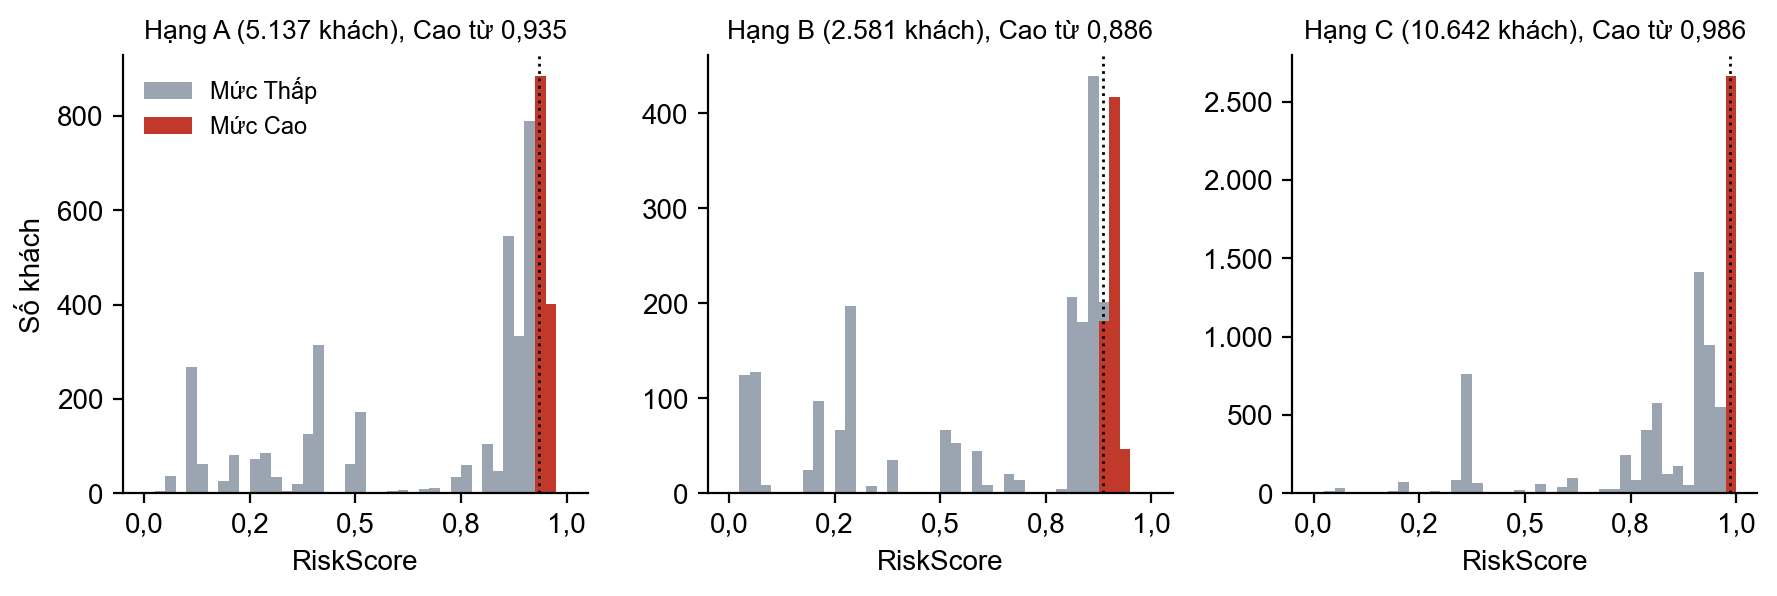
\includegraphics[width=0.95\textwidth]{m_diem_theo_hang.png}
\caption{Phân bố \texttt{RiskScore} của khách mức Cao và mức Thấp theo hạng ABC}
\label{fig:diemhang}
\end{figure}

\begin{figure}[!htbp]
\centering
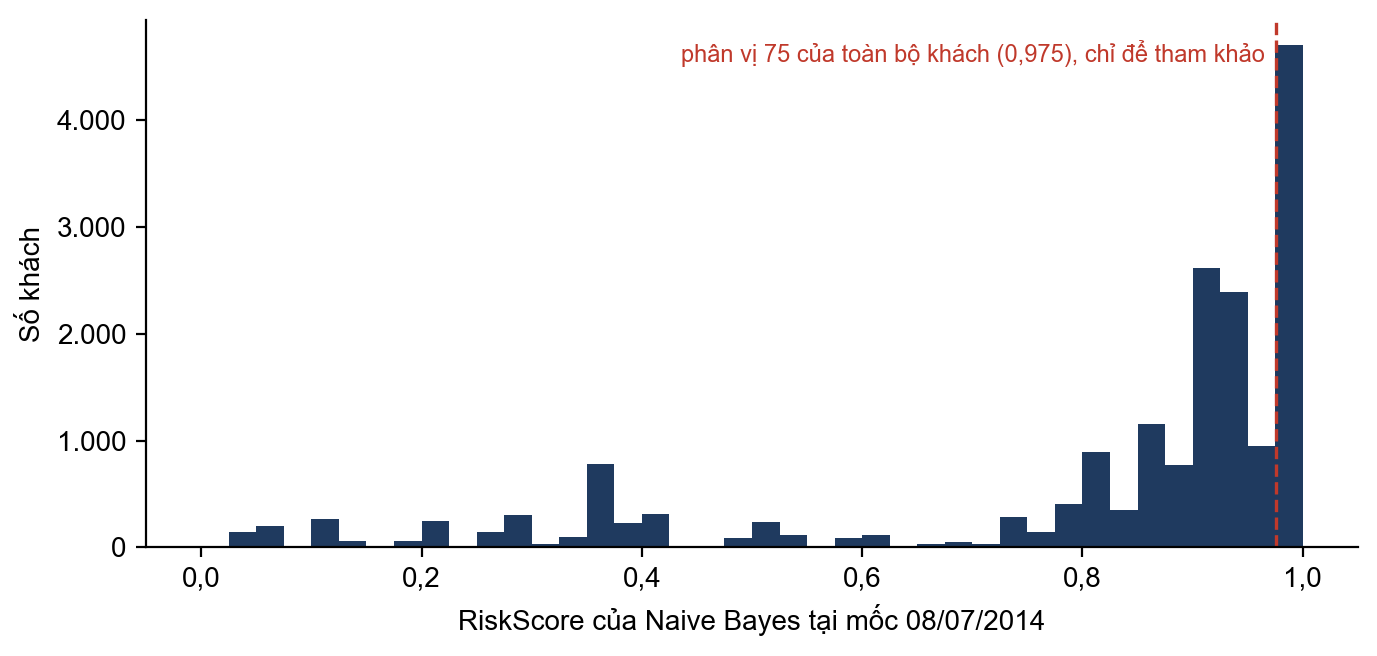
\includegraphics[width=0.55\textwidth]{m_phan_bo_diem.png}
\caption{Phân bố \texttt{RiskScore} trên 18.360 khách tại mốc 08/07/2014}
\label{fig:phanbo_diem}
\end{figure}
\FloatBarrier

\clearpage
% Chương Hệ hỗ trợ ra quyết định
% Số liệu lấy từ results/cum6 và results/cum6b. Bảng d_*.tex do python/tao_bang_tex_dss.py sinh, hình d_chon_k.png và d_man_hinh_*.png do python/ve_hinh_dss.py sinh.
% Hình d_do_nhay.png và d_mo_phong.png do python/ve_hinh_mohinh.py sinh. Không sửa tay số liệu trong latex/bang/.
% Mỗi mục đi theo một câu hỏi của người quản lý, thiết kế và kết quả chạy thật viết chung.
\section{Thiết kế và hiện thực hệ hỗ trợ ra quyết định}

Chương 5 cho ra xác suất không mua lại của từng khách. Chương này biến xác suất đó thành quyết định. Người quản lý cần trả lời bốn câu hỏi: chọn khách nào trong ngân sách (mục 6.2), khách thuộc nhóm nào (6.3), chăm sóc bằng cách nào (6.4) và đặt ngân sách bao nhiêu khi chưa biết chăm sóc có hiệu quả không (6.5). Mục 6.1 nêu bài toán và kiến trúc, mục 6.6 trình bày giao diện và bản demo. Trừ khi nói khác, số liệu tính tại mốc chấm điểm 08/07/2014 cho 18.360 khách.

\subsection{Bài toán và kiến trúc DSS}
\subsubsection{Quyết định cần hỗ trợ}
Tại mỗi mốc chấm điểm, với một ngân sách có hạn, người quản lý phải chọn khách nào cần chăm sóc trong 90 ngày tiếp theo và chăm sóc bằng hành động nào. Phải chọn vì không thể chăm sóc tất cả: ngân sách có hạn và 81,2\% khách có nhãn không mua lại (Bảng~\ref{tab:thamso}). Đây là quyết định bán cấu trúc ở cấp quản lý~\cite{turban2011}. Phần có cấu trúc (tính xác suất, giá trị kỳ vọng, chọn khách trong ngân sách) do máy làm. Phần không có cấu trúc (chọn hình thức chăm sóc, cân nhắc thông tin ngoài dữ liệu, chốt ngân sách) do người quản lý làm. Ba nhóm người dùng là quản lý Marketing/Sales (đặt ngân sách, chạy kịch bản, duyệt danh sách), nhân viên phân tích dữ liệu (chấm điểm, theo dõi mô hình, đề xuất quy tắc) và nhân viên chăm sóc khách hàng (thực hiện theo danh sách).

Hai nguyên tắc thiết kế xuyên suốt. Thứ nhất, DSS đề xuất, người dùng quyết định cuối, và người dùng xem được theo rủi ro, theo giá trị hay theo nhóm tuỳ ý~\cite{turban2011}. Thứ hai, xác suất không mua lại chỉ cho biết khách có nguy cơ, không cho biết chăm sóc có làm khách quay lại hay không~\cite{lemmens2020}, nên hiệu quả chăm sóc là tham số do người quản lý giả định và được thử ở mục 6.5.

\subsubsection{Bốn thành phần và bốn pha ra quyết định}
CompanyX DSS gồm bốn thành phần đúng như Chương 2~\cite{tlmh,turban2011} (Bảng~\ref{tab:thanhphan}), mở rộng từ khung dữ liệu, mô hình và giao diện của Sprague~\cite{sprague1980}. Bảng~\ref{tab:quytrinh} ánh xạ bốn pha của Simon~\cite{simon1977,turban2011} (Hình~\ref{fig:simon}) vào câu hỏi của người quản lý và chức năng tương ứng của DSS. Việc gửi chiến dịch nằm ngoài hệ thống, DSS chỉ cung cấp danh sách và khuyến nghị.

\begin{table}[!htbp]
\centering
\caption{Bốn thành phần của CompanyX DSS}
\label{tab:thanhphan}
\footnotesize
\begin{tabular}{p{2.8cm}p{11.6cm}}
\toprule
Thành phần & Nội dung \\
\midrule
Quản lý dữ liệu & Đọc kho \texttt{CompanyX\_DW}, chủ yếu các bảng \texttt{analytics.\allowbreak CustomerSnapshot}, \texttt{analytics.\allowbreak CustomerRiskScore}, và ghi kết quả vào \texttt{CustomerSegment}, \texttt{CareRecommendation} \\
Quản lý mô hình & Naive Bayes (Chương 5), K-means, mô hình giá trị ròng kỳ vọng và bài toán chọn khách trong ngân sách \\
Quản lý tri thức & Kho quy tắc chăm sóc R1 đến R9 (bảng \texttt{analytics.\allowbreak CareRule}) và luật kết hợp gợi ý sản phẩm \\
Giao diện người dùng & Ứng dụng web Streamlit~\cite{streamlit}, cho đổi giả định mà không cần huấn luyện lại mô hình \\
\bottomrule
\end{tabular}
\end{table}

\begin{table}[!htbp]
\centering
\caption{Bốn pha ra quyết định và chức năng DSS hỗ trợ}
\label{tab:quytrinh}
\footnotesize
\begin{tabular}{p{1.9cm}p{3.9cm}p{5.8cm}p{2.2cm}}
\toprule
Pha & Câu hỏi của người quản lý & Chức năng DSS & Mục \\
\midrule
Tìm hiểu & Tình hình khách không mua lại ra sao, nhóm nào đáng lo? & Dashboard tổng quan: tỷ lệ nguy cơ, phân bố xác suất, hạng giá trị, nhóm khách & 6.3 \\
Thiết kế & Có những phương án nào, mỗi phương án cho kết quả ra sao? & Mô hình giá trị kỳ vọng, what-if, độ nhạy & 6.2, 6.5 \\
Lựa chọn & Chọn khách nào, bao nhiêu khách? & Tối ưu trong ngân sách, tìm mục tiêu, danh sách ưu tiên & 6.2, 6.4 \\
Thực hiện & Làm gì với từng khách, kết quả ra sao? & Khuyến nghị theo quy tắc, xuất danh sách, theo dõi mô hình & 6.4, 6.6 \\
\bottomrule
\end{tabular}
\end{table}

\subsection{Chọn khách nào trong ngân sách}
\subsubsection{Giá trị kỳ vọng của việc chăm sóc một khách}
Mô hình xét một lát cắt tại mốc chấm điểm và một chu kỳ 90 ngày sau mốc. Việc khách $i$ có mua lại hay không ($Y_i$) là điều kiện rủi ro: chưa biết trước nhưng có xác suất $p_i$ từ Chương 5. Tỷ lệ chăm sóc thành công $r$ và chi phí $c$ là điều kiện bất định vì chưa có chiến dịch nào để đo, nên người quản lý nhập theo giả định. Bảng~\ref{tab:bien} liệt kê các biến theo ba loại ở Chương 2, thêm biến trung gian, Hình~\ref{fig:influence} vẽ quan hệ giữa chúng: hình chữ nhật là biến quyết định, hình tròn là biến không kiểm soát được hoặc trung gian, hình bầu dục là biến kết quả, mũi tên gấp khúc là quan hệ rủi ro hoặc bất định.

\begin{table}[!htbp]
\centering
\caption{Các biến của mô hình quyết định chăm sóc khách hàng}
\label{tab:bien}
\footnotesize
\begin{tabular}{p{2.4cm}p{1.8cm}p{6.2cm}p{3.8cm}}
\toprule
Loại biến & Ký hiệu & Ý nghĩa & Nguồn hoặc giá trị \\
\midrule
Biến quyết định & $x_i$ & Chăm sóc khách $i$ ($x_i=1$) hay không ($x_i=0$) & Lời giải của mô hình, người quản lý duyệt \\
Không kiểm soát được & $B$ & Ngân sách chiến dịch, cố định trong một lần giải & Người quản lý nhập \\
Không kiểm soát được & $Y_i$ & Khách $i$ không có đơn hợp lệ trong 90 ngày sau mốc (giá trị quan sát được sau này là nhãn $y_i$ ở Chương 4) & Chưa biết tại mốc \\
Không kiểm soát được & $p_i$ & Xác suất $Y_i=1$ do mô hình phân lớp dự đoán & \texttt{RiskScore} \\
Không kiểm soát được & $AOV_i$ & Giá trị trung bình một đơn của khách $i$ trước mốc (\texttt{SubTotal}, không gồm thuế và phí vận chuyển) & \texttt{FactSalesOrder} \\
Không kiểm soát được & $g$ & Tỷ lệ lợi nhuận gộp trên doanh thu & Tính từ giá vốn các đơn trước mốc \\
Không kiểm soát được & $r$ & Tỷ lệ chăm sóc thành công: xác suất một khách vốn sẽ không mua lại quay lại mua nhờ được chăm sóc & Giả định, người quản lý nhập \\
Không kiểm soát được & $c$ & Chi phí cho mỗi khách được chọn (liên hệ và ưu đãi) & Giả định, người quản lý nhập \\
Trung gian & $v_i=g\cdot AOV_i$ & Lợi nhuận gộp của một lần mua nếu giữ được khách $i$ & Tính từ $AOV_i$ và $g$ \\
Kết quả & $Z=R-C$ & Giá trị ròng kỳ vọng: lợi nhuận gộp kỳ vọng giữ lại $R$ trừ tổng chi phí $C$ & Tính từ mô hình \\
\bottomrule
\end{tabular}
\end{table}

\begin{figure}[!htbp]
\centering
\begin{tikzpicture}[
  dec/.style={draw, rectangle, minimum width=1.0cm, minimum height=0.7cm, font=\small},
  var/.style={draw, circle, minimum size=1.0cm, inner sep=1pt, font=\small},
  res/.style={draw, ellipse, minimum width=1.5cm, minimum height=0.9cm, font=\small},
  cert/.style={-{Stealth[length=2mm]}},
  risk/.style={-{Stealth[length=2mm]}, decorate, decoration={zigzag, amplitude=0.8pt, segment length=4pt}}]
  \node[var] (g) at (0,3.6) {$g$};
  \node[var] (aov) at (0,2.2) {$AOV_i$};
  \node[var] (p) at (0,0.5) {$p_i$};
  \node[var] (y) at (0,-1.0) {$\tilde{Y}_i$};
  \node[var] (r) at (0,-2.5) {$r$};
  \node[var] (v) at (3.0,3.0) {$v_i$};
  \node[var] (R) at (6.0,0.4) {$R$};
  \node[dec] (x) at (3.0,-3.0) {$x_i$};
  \node[var] (B) at (0,-4.2) {$B$};
  \node[var] (c) at (3.0,-5.2) {$c$};
  \node[var] (C) at (6.0,-3.6) {$C$};
  \node[res] (Z) at (9.2,-1.6) {$Z$};
  \draw[cert] (g) -- (v);
  \draw[cert] (aov) -- (v);
  \draw[cert] (v) -- (R);
  \draw[cert] (p) -- (y);
  \draw[risk] (y) -- (R);
  \draw[risk] (r) -- (R);
  \draw[cert] (x) -- (R);
  \draw[cert] (x) -- (C);
  \draw[cert] (c) -- (C);
  \draw[cert] (B) -- node[above, font=\scriptsize] {ràng buộc} (x);
  \draw[cert] (R) -- (Z);
  \draw[cert] (C) -- (Z);
\end{tikzpicture}

\caption{Sơ đồ ảnh hưởng của mô hình quyết định chăm sóc khách hàng}
\label{fig:influence}
\end{figure}

Với một khách $i$ có hai phương án: chăm sóc hoặc không. Bảng~\ref{tab:payoffhai} tính kết quả của hai phương án theo hai trạng thái của khách, lấy chênh lệch so với không chăm sóc. Bảng dựa trên hai giả định: $r$ chỉ tính trên khách sẽ rời bỏ nếu không được chăm sóc, và chăm sóc không đổi hành vi của khách vốn sẽ quay lại.

\begin{table}[!htbp]
\centering
\caption{Bảng kết quả của hai phương án đối với khách $i$}
\label{tab:payoffhai}
\footnotesize
\begin{tabular}{p{3.0cm}p{4.0cm}p{4.0cm}p{2.8cm}}
\toprule
Phương án & Khách sẽ rời bỏ (xác suất $p_i$) & Khách vẫn quay lại (xác suất $1-p_i$) & Giá trị kỳ vọng \\
\midrule
Không chăm sóc & 0 & 0 & 0 \\
Chăm sóc & $r\, v_i - c$ & $-c$ & $p_i\, r\, v_i - c$ \\
\bottomrule
\end{tabular}
\end{table}

Giá trị kỳ vọng của việc chăm sóc khách $i$ và tiêu chí chọn khách là:
\begin{align}
    v_i &= g \cdot AOV_i, \qquad EV_i = p_i\, r\, v_i - c \label{eq:EV}\\
    \text{chọn chăm sóc khách } i \text{ khi } EV_i > 0 &\iff p_i\, v_i > c/r \quad (r>0) \label{eq:chon}
\end{align}
Ví dụ với $r=10\%$, $c=10$ USD (nên $c/r=100$ USD) và $g=40\%$ (giá trị minh hoạ):
\begin{itemize}
    \item Khách A: $p_i=0{,}90$, $AOV_i=2.500$ USD, $v_i=1.000$ USD, $EV_i=0{,}90 \times 0{,}10 \times 1.000 - 10 = 80$ USD, chọn.
    \item Khách B: $p_i=0{,}98$, $AOV_i=40$ USD, $v_i=16$ USD, $EV_i=0{,}98 \times 0{,}10 \times 16 - 10 = -8{,}43$ USD, không chọn.
    \item Khách C: $p_i=0{,}50$, $AOV_i=2.000$ USD, $v_i=800$ USD, $EV_i=0{,}50 \times 0{,}10 \times 800 - 10 = 30$ USD, chọn.
\end{itemize}
Khách B có xác suất rời bỏ cao nhất nhưng không đáng chăm sóc vì giá trị quá nhỏ. Vì vậy xác suất chỉ là đầu vào, việc chọn khách dựa trên giá trị kỳ vọng. Do $p_i$ nhân thẳng vào $EV_i$, mô hình cần xác suất sát thực tế, đây là lý do Chương 5 theo dõi Brier.

\subsubsection{Bài toán tối ưu và cách giải}
Cộng giá trị kỳ vọng của các khách được chọn ta có $Z$. Bài toán là quy hoạch nguyên 0--1, cùng cấu trúc với bài toán phối hợp sản phẩm ở Chương 2~\cite{turban2011}:
\begin{align}
    \max\; Z &= R - C = \sum_i x_i\, p_i\, r\, v_i - c \sum_i x_i = \sum_i x_i\,(p_i\, r\, v_i - c) \label{eq:muctieu}\\
    \text{với}\quad & c \sum_i x_i \leq B, \qquad x_i \in \{0,1\} \label{eq:rangbuoc}
\end{align}
Chương 5 tính cùng công thức $Z$ với nhãn thật $y_i$ thay cho $p_i$ để so các mô hình. Vì chi phí $c$ như nhau cho mọi khách, lời giải tối ưu là xếp khách theo $p_i v_i$ giảm dần và chọn $K$ khách đầu:
\begin{equation}
    K = \min\left(\lfloor B/c \rfloor,\; n_+\right) \label{eq:K}
\end{equation}
với $\lfloor B/c \rfloor$ là số khách ngân sách cho phép và $n_+$ là số khách có $EV_i>0$. Khi chi phí khác nhau giữa các khách (mục 6.4.3), bài toán thành bài toán cái túi 0--1 và được giải bằng quy hoạch nguyên.

Mô hình có ba giới hạn cần nhớ. $p_i$ học từ lịch sử không có chiến dịch giữ chân nào, nên $Z$ là giá trị kỳ vọng theo giả định, không phải hiệu quả đã đo, muốn đo thật cần chiến dịch có nhóm đối chứng~\cite{lemmens2020}. $v_i$ chỉ tính một lần mua với một tỷ lệ lợi nhuận gộp chung, không phải giá trị vòng đời. $c$ phát sinh cả với khách vốn sẽ quay lại.

\subsubsection{Các đại lượng đo từ dữ liệu}
Bảng~\ref{tab:thamso} là các đại lượng đo được từ kho. Khách không mua lại chiếm 81,2\% (trung bình 19 mốc có nhãn) nên không thể chăm sóc tất cả. 50,5\% khách có $v_i$ nhỏ hơn $c/r = 100$ USD, tức chăm sóc riêng không bù được chi phí. Nếu không tính lợi ích từ khách chưa đến kỳ mua lại, $Z$ cơ sở còn 205.555 USD, nên các giá trị $Z$ dưới đây là cận trên.

\begin{table}[!htbp]
\centering
\caption{Các đại lượng của mô hình giá trị kỳ vọng đo từ dữ liệu}
\label{tab:thamso}
\footnotesize
\begin{tabular}{p{4.6cm}p{3.6cm}p{6.2cm}}
\toprule
Đại lượng & Giá trị & Ghi chú \\
\midrule
Tỷ lệ lợi nhuận gộp g, toàn bộ & 0,4115 & Giá vốn ProductCostHistory tại ngày đặt, 59.795 dòng trong phạm vi \\
g của Bikes / Accessories / Clothing & 0,406 / 0,626 / 0,402 & Bikes chiếm 96,5\% doanh thu \\
Z kịch bản cơ sở nếu dùng g theo nhóm & 290.014 USD (g chung 292.595 USD) & 99,7\% khách trong danh sách giữ nguyên \\
Tỷ lệ khách không mua lại trong 90 ngày ($y=1$) & 81,2\% & Trung bình 19 mốc có nhãn \\
Tỷ trọng Monetary của khách $y=1$ & 78,0\% & Trung bình 19 mốc có nhãn \\
Số đơn trung bình của khách quay lại trong 90 ngày & 1,12 & 93,5\% chỉ đặt một đơn \\
Giá trị đơn khi quay lại so với AOV trước đó (trung vị tỷ số) & 0,87 & Trung bình 1.427 USD so với 1.873 USD \\
Khách có v $<$ c/r = 100 USD tại mốc chấm điểm & 50,5\% & Chăm sóc riêng không bù được chi phí \\
Z cơ sở nếu trừ khách chưa đến kỳ khỏi lợi ích & 205.555 USD (r hoà vốn 1,63\%) & 26,2\% khách $y=1$ theo nhãn 90 ngày tự mua lại trong ngày 90–180 \\
Ngân sách để kênh R4 (nhóm N3) bắt đầu có khách & khoảng 61.213 USD & Dưới mức này lợi trên mỗi USD của khách N3 thấp hơn khách khác \\
\bottomrule
\end{tabular}

\end{table}

\subsubsection{Kết quả kịch bản cơ sở và what-if}
Kịch bản cơ sở là $r=10\%$, $c=10$ USD mỗi khách và $B=40.000$ USD. Với kịch bản này hệ thống chọn 4.000 khách, kỳ vọng giữ lại 358 khách và đạt $Z = 292.595$ USD. Với what-if, người quản lý đổi một tham số rồi xem kết quả (Bảng~\ref{tab:whatif}, Hình~\ref{fig:man3}). Tăng $r$ từ 10\% lên 20\% làm $Z$ tăng lên 625.189 USD, nên tỷ lệ thành công là yếu tố ảnh hưởng lớn nhất. Tăng ngân sách lên 100.000 USD thì DSS chỉ dùng 85.540 USD vì đã hết khách có $EV$ dương. Mỗi lần phân tích, DSS lưu tham số và kết quả thành một kịch bản để so sánh.

\begin{table}[!htbp]
\centering
\caption{Phân tích what-if quanh kịch bản cơ sở}
\label{tab:whatif}
\footnotesize
\resizebox{\textwidth}{!}{\begin{tabular}{lrrrr}
\toprule
Kịch bản & Số khách & Chi phí (USD) & $Z$ (USD) & Chênh so với cơ sở (USD) \\
\midrule
Cơ sở ($r=10\%$, $c=10$ USD, $B=40.000$ USD) & 4.000 & 40.000 & 292.595 & 0 \\
$r=5\%$ & 4.000 & 40.000 & 126.297 & $-$166.297 \\
$r=20\%$ & 4.000 & 40.000 & 625.189 & +332.595 \\
$c=5$ USD & 8.000 & 40.000 & 424.359 & +131.764 \\
$c=20$ USD & 2.000 & 40.000 & 152.066 & $-$140.529 \\
$B=20.000$ USD & 2.000 & 20.000 & 172.066 & $-$120.529 \\
$B=60.000$ USD & 6.000 & 60.000 & 359.388 & +66.793 \\
$B=100.000$ USD & 8.554 & 85.540 & 386.235 & +93.640 \\
\bottomrule
\end{tabular}
}
\end{table}

\begin{figure}[!htbp]
\centering
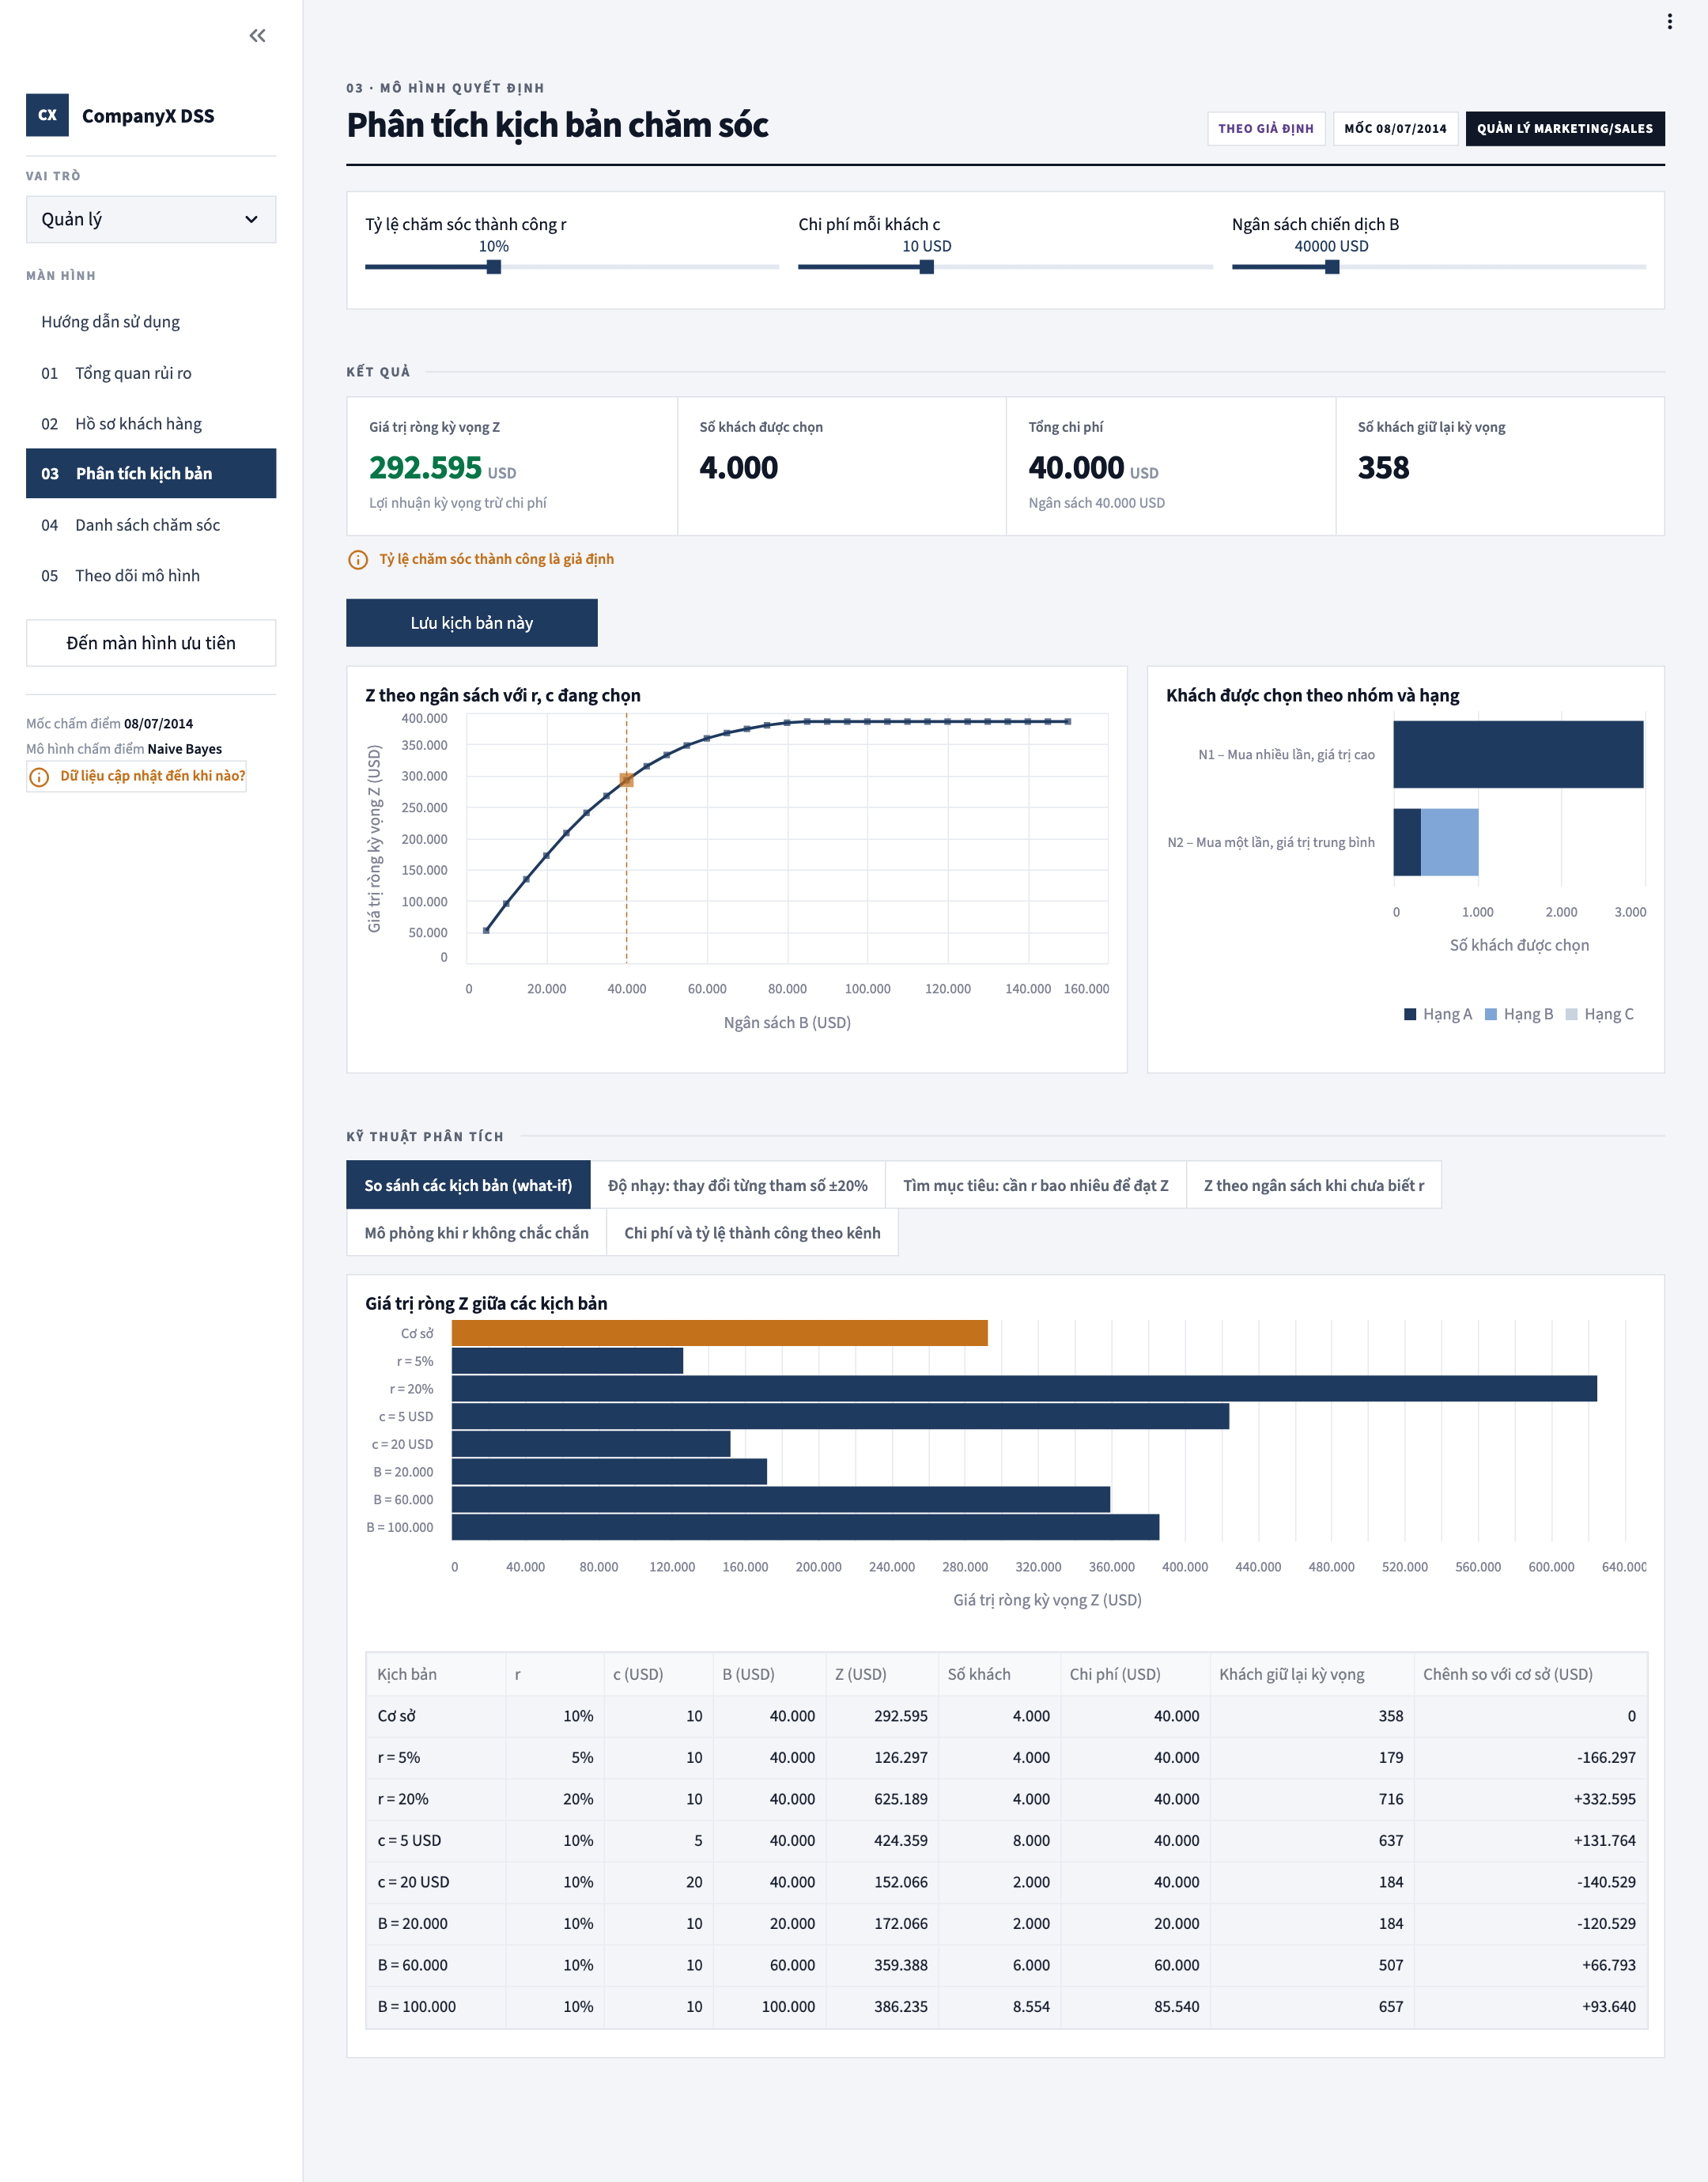
\includegraphics[width=0.95\textwidth]{d_man_hinh_3.png}
\caption{Màn hình 3: phân tích kịch bản và sự thay đổi giá trị ròng kỳ vọng trên DSS}
\label{fig:man3}
\end{figure}

\subsection{Khách thuộc nhóm nào}
Để người quản lý nắm cơ cấu khách và chọn cách chăm sóc phù hợp, DSS chia khách theo hai cách: hạng ABC theo giá trị và nhóm hành vi theo RFM. Cả hai tính tại mốc chấm điểm, chỉ dùng đơn trước mốc, không dùng nhãn. Nhóm và hạng không đổi danh sách chọn theo giá trị kỳ vọng, chúng dùng để mô tả trên dashboard và để chọn hình thức chăm sóc trong kho quy tắc. Kết quả ghi vào \texttt{analytics.\allowbreak CustomerSegment}, mô hình gom cụm lưu trong \texttt{analytics.\allowbreak ModelRegistry} và học lại cùng chu kỳ với mô hình phân lớp.

\subsubsection{Phân hạng ABC theo giá trị}
Phân tích ABC (mục~\ref{sec:rfmabc}) xếp khách theo Monetary (tổng \texttt{TotalDue} trước mốc) giảm dần rồi tính tỷ trọng luỹ kế:
\begin{equation}
    S_k = \frac{M_{(1)} + M_{(2)} + \dots + M_{(k)}}{\sum_i M_i} \label{eq:abc}
\end{equation}
Khách thứ $k$ thuộc hạng A nếu $S_{k-1} < 80\%$, hạng B nếu $80\% \leq S_{k-1} < 95\%$, còn lại là hạng C. Kết quả là 5.137 khách hạng A, 2.581 hạng B và 10.642 hạng C (Bảng~\ref{tab:abc}). Hạng B có xác suất không mua lại trung bình thấp nhất (0,665), hạng A ở giữa (0,749) và hạng C cao nhất (0,867). Mức rủi ro Cao tính theo phân vị trong từng hạng (Chương 5) cho 4.592 khách: hạng A 1.285, hạng B 646, hạng C 2.661. Ghép mức rủi ro với hạng ABC được ma trận Rủi ro $\times$ Giá trị trên dashboard, giúp nhìn cùng lúc nguy cơ và giá trị, ví dụ ô hạng A rủi ro Cao là nhóm cần xem trước khi lập chiến dịch.

\begin{table}[!htbp]
\centering
\caption{Phân hạng ABC theo Monetary tại mốc 08/07/2014}
\label{tab:abc}
\footnotesize
\begin{tabular}{lR{1.5cm}R{1.5cm}R{1.9cm}R{2.2cm}R{2.1cm}R{2.2cm}}
\toprule
Hạng & Số khách & Tỷ lệ khách & Tỷ trọng Monetary & Monetary trung vị (USD) & RiskScore trung bình & $v$ trung vị (USD) \\
\midrule
Hạng A & 5.137 & 28,0\% & 80\% & 4.859,51 & 0,749 & 938,42 \\
Hạng B & 2.581 & 14,1\% & 15\% & 1.918,26 & 0,665 & 493,38 \\
Hạng C & 10.642 & 58,0\% & 5\% & 71,01 & 0,867 & 20,56 \\
\bottomrule
\end{tabular}

\end{table}

Ngưỡng 80\%/95\% là quy ước, không tối ưu từ dữ liệu. Khi thử ngưỡng 70\%/90\% (Bảng~\ref{tab:abcnguong}), 2.278 khách đổi hạng nhưng danh sách theo kênh chỉ đổi từ 6.124 lên 6.480 khách và $Z$ giảm 1.802 USD (khoảng 0,7\%). Quyết định gần như không đổi nên nhóm giữ ngưỡng 80\%/95\%.

\begin{table}[!htbp]
\centering
\caption{Độ nhạy theo ngưỡng ABC: 80\%/95\% so với 70\%/90\%}
\label{tab:abcnguong}
\footnotesize
\begin{tabular}{lrr}
\toprule
Chỉ số & Ngưỡng 80\%/95\% (thiết kế) & Ngưỡng 70\%/90\% \\
\midrule
Số khách hạng A / B / C & 5.137 / 2.581 / 10.642 & 4.019 / 2.539 / 11.802 \\
Khách mức Cao hạng A / B / C & 1.285 / 646 / 2.661 & 1.005 / 635 / 2.951 \\
Khách đủ điều kiện R3 & 1.647 & 1.499 \\
Khách được chọn R3 / R5 & 983 / 5.141 & 934 / 5.546 \\
Tổng khách được chọn & 6.124 & 6.480 \\
Chi phí (USD) & 39.998 & 39.988 \\
$Z$ (USD) & 256.502 & 254.700 \\
Chênh $Z$ so với thiết kế (USD) & 0 & $-$1.802 \\
Số khách đổi hạng & 0 & 2.278 \\
\bottomrule
\end{tabular}

\end{table}

\subsubsection{Năm nhóm hành vi bằng K-means}
Nhóm chọn K-means~\cite{han2011} vì chạy nhanh với vài chục nghìn khách, mỗi nhóm có tâm nên dễ diễn giải, và khách mới được gán vào nhóm gần nhất mà không cần chạy lại. Đặc trưng là Recency, Frequency và Monetary tại mốc. Frequency và Monetary lệch phải mạnh nên lấy $\ln(1+x)$, rồi cả ba chuẩn hoá z-score để không đặc trưng nào lấn át khoảng cách. Thống kê Hopkins (đo mức dữ liệu tụ thành cụm, gần 0 là có cụm, 0,5 là phân bố ngẫu nhiên) bằng 0,004, cho thấy dữ liệu có cấu trúc cụm rõ. Số cụm chọn từ 2 đến 10 bằng đường Elbow và hệ số Silhouette~\cite{rousseeuw1987}, với yêu cầu số nhóm đủ ít để đặt tên và gắn quy tắc. Đường WCSS (tổng bình phương khoảng cách trong cụm) gãy trong khoảng $k=3$ đến 5, trong khoảng này $k=5$ có Silhouette cao nhất (0,466) (Bảng~\ref{tab:chonk}, Hình~\ref{fig:chonk}). Các $k$ lớn hơn có Silhouette nhỉnh hơn một chút nhưng nhóm nhỏ dần, nên nhóm chọn $k=5$. Kết quả ổn định: chỉ số Adjusted Rand Index~\cite{hubert1985} (đo mức giống nhau giữa hai cách chia nhóm, 1 là trùng khớp) bằng 1,0 với ba lần khởi tạo khác và 0,995 khi so với gom cụm phân cấp Ward.

\begin{table}[!htbp]
\centering
\caption{Chọn số cụm $k$: WCSS và Silhouette}
\label{tab:chonk}
\footnotesize
\begin{tabular}{crr}
\toprule
$k$ & WCSS & Silhouette \\
\midrule
2 & 34.456,1 & 0,412 \\
3 & 25.155,1 & 0,449 \\
4 & 18.689,9 & 0,409 \\
5 & 14.784,0 & 0,466 \\
6 & 12.019,8 & 0,452 \\
7 & 10.204,1 & 0,460 \\
8 & 8.517,2 & 0,471 \\
9 & 6.951,6 & 0,455 \\
10 & 5.878,5 & 0,481 \\
\bottomrule
\end{tabular}

\end{table}

\begin{figure}[!htbp]
\centering
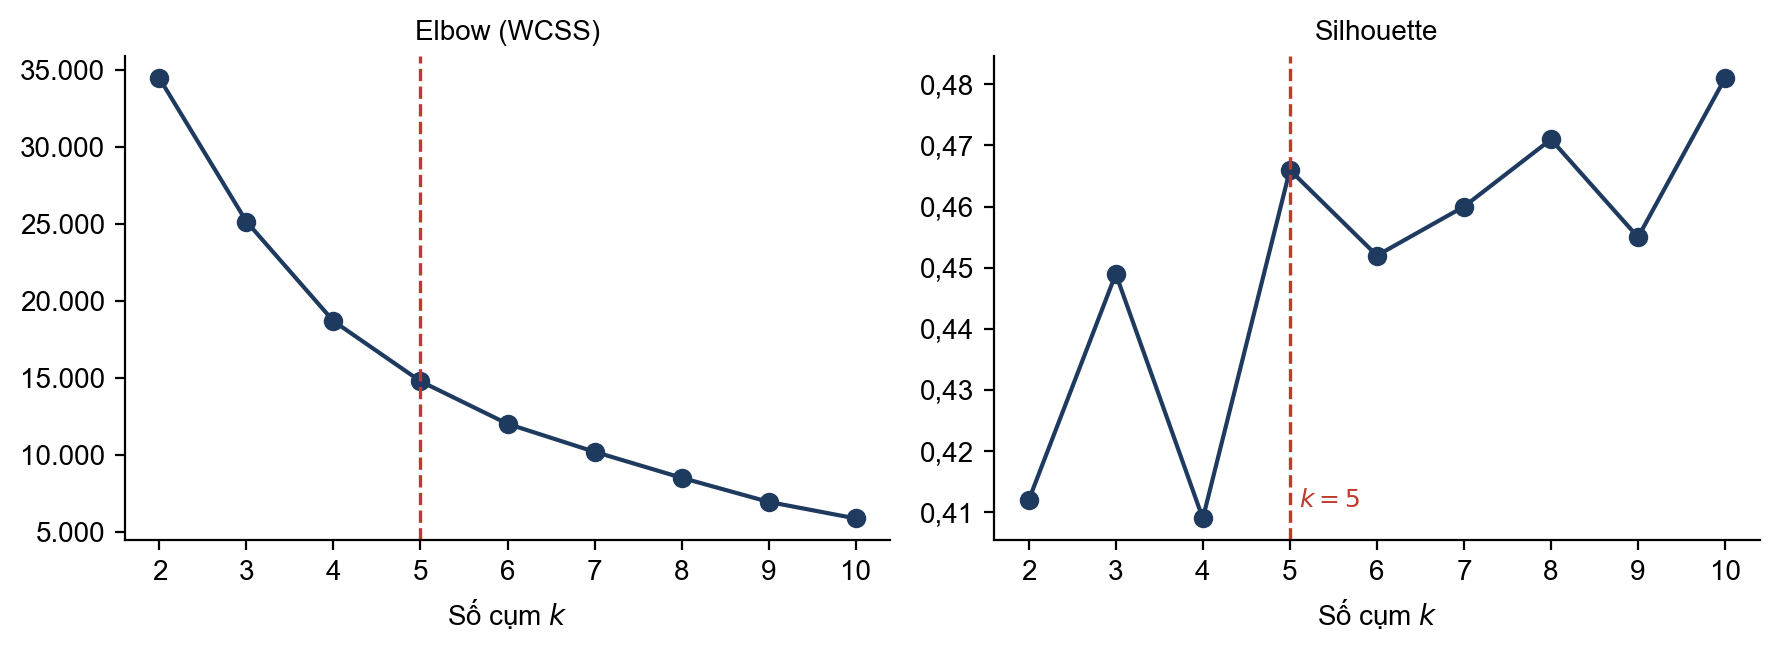
\includegraphics[width=0.8\textwidth]{d_chon_k.png}
\caption{Elbow và Silhouette khi chọn số cụm $k$}
\label{fig:chonk}
\end{figure}

Mỗi nhóm được đặt tên theo mức Recency, Frequency, Monetary so với các nhóm còn lại (Bảng~\ref{tab:honhom}).
\begin{itemize}
    \item \textbf{N1, mua nhiều lần, giá trị cao:} 4.926 khách (26,8\%), mua trung bình 2,2 lần, Monetary trung vị 4.910 USD, giữ 75,6\% tổng giá trị.
    \item \textbf{N2, mua một lần, giá trị trung bình:} 3.741 khách (20,4\%).
    \item \textbf{N3, mua một lần, đã lâu không quay lại:} 428 khách (2,3\%), Recency trung vị 917,5 ngày.
    \item \textbf{N4, mua lặp lại, giá trị thấp:} 1.839 khách (10,0\%), mua 2,7 lần nhưng chủ yếu là phụ kiện, Monetary trung vị chỉ 118 USD.
    \item \textbf{N5, mua một lần, giá trị thấp:} 7.426 khách (40,4\%), đông nhất, mua khoảng 44 USD.
\end{itemize}
N1 và N2 chiếm khoảng 93,6\% tổng Monetary. Hai dòng cuối của Bảng~\ref{tab:honhom} cho thấy nhóm nào được chọn chăm sóc. N4 và N5 không có khách nào $EV$ dương vì giá trị một lần mua quá nhỏ so với chi phí. N3 có 62,6\% khách $EV$ dương nhưng không khách nào được chọn ở ngân sách cơ sở, vì lợi trên mỗi USD thấp hơn các nhóm khác. Danh sách cuối chỉ gồm N1 (3.964 khách) và N2 (2.160 khách), đúng ý đồ dồn ngân sách vào khách có giá trị. Hình~\ref{fig:man1} là màn hình tổng quan trình bày các kết quả này.

\begin{table}[!htbp]
\centering
\caption{Hồ sơ năm nhóm khách hàng K-means tại mốc 08/07/2014}
\label{tab:honhom}
\footnotesize
\resizebox{\textwidth}{!}{\begin{tabular}{lrrrrr}
\toprule
Chỉ số & N1 & N2 & N3 & N4 & N5 \\
\midrule
Số khách & 4.926 & 3.741 & 428 & 1.839 & 7.426 \\
Tỷ lệ khách & 26,8\% & 20,4\% & 2,3\% & 10,0\% & 40,4\% \\
Recency trung vị (ngày) & 170 & 183 & 917,5 & 100 & 191 \\
Frequency trung bình & 2,21 & 1,00 & 1,00 & 2,66 & 1,00 \\
Monetary trung vị (USD) & 4.909,93 & 1.297,80 & 3.953,99 & 117,96 & 44,18 \\
Tỷ trọng Monetary & 75,6\% & 18,0\% & 4,3\% & 0,9\% & 1,3\% \\
Khách hạng A / B / C & 4.280 / 645 / 1 & 561 / 1.810 / 1.370 & 296 / 102 / 30 & 0 / 24 / 1.815 & 0 / 0 / 7.426 \\
RiskScore trung bình & 0,806 & 0,702 & 0,100 & 0,969 & 0,858 \\
Tỷ lệ mức Cao & 33,4\% & 7,0\% & 0,0\% & 55,2\% & 22,5\% \\
Tỷ lệ khách $EV>0$ & 98,7\% & 91,6\% & 62,6\% & 0,0\% & 0,0\% \\
Được chọn theo kênh & 3.964 & 2.160 & 0 & 0 & 0 \\
\bottomrule
\end{tabular}
}
\end{table}

\begin{figure}[!htbp]
\centering
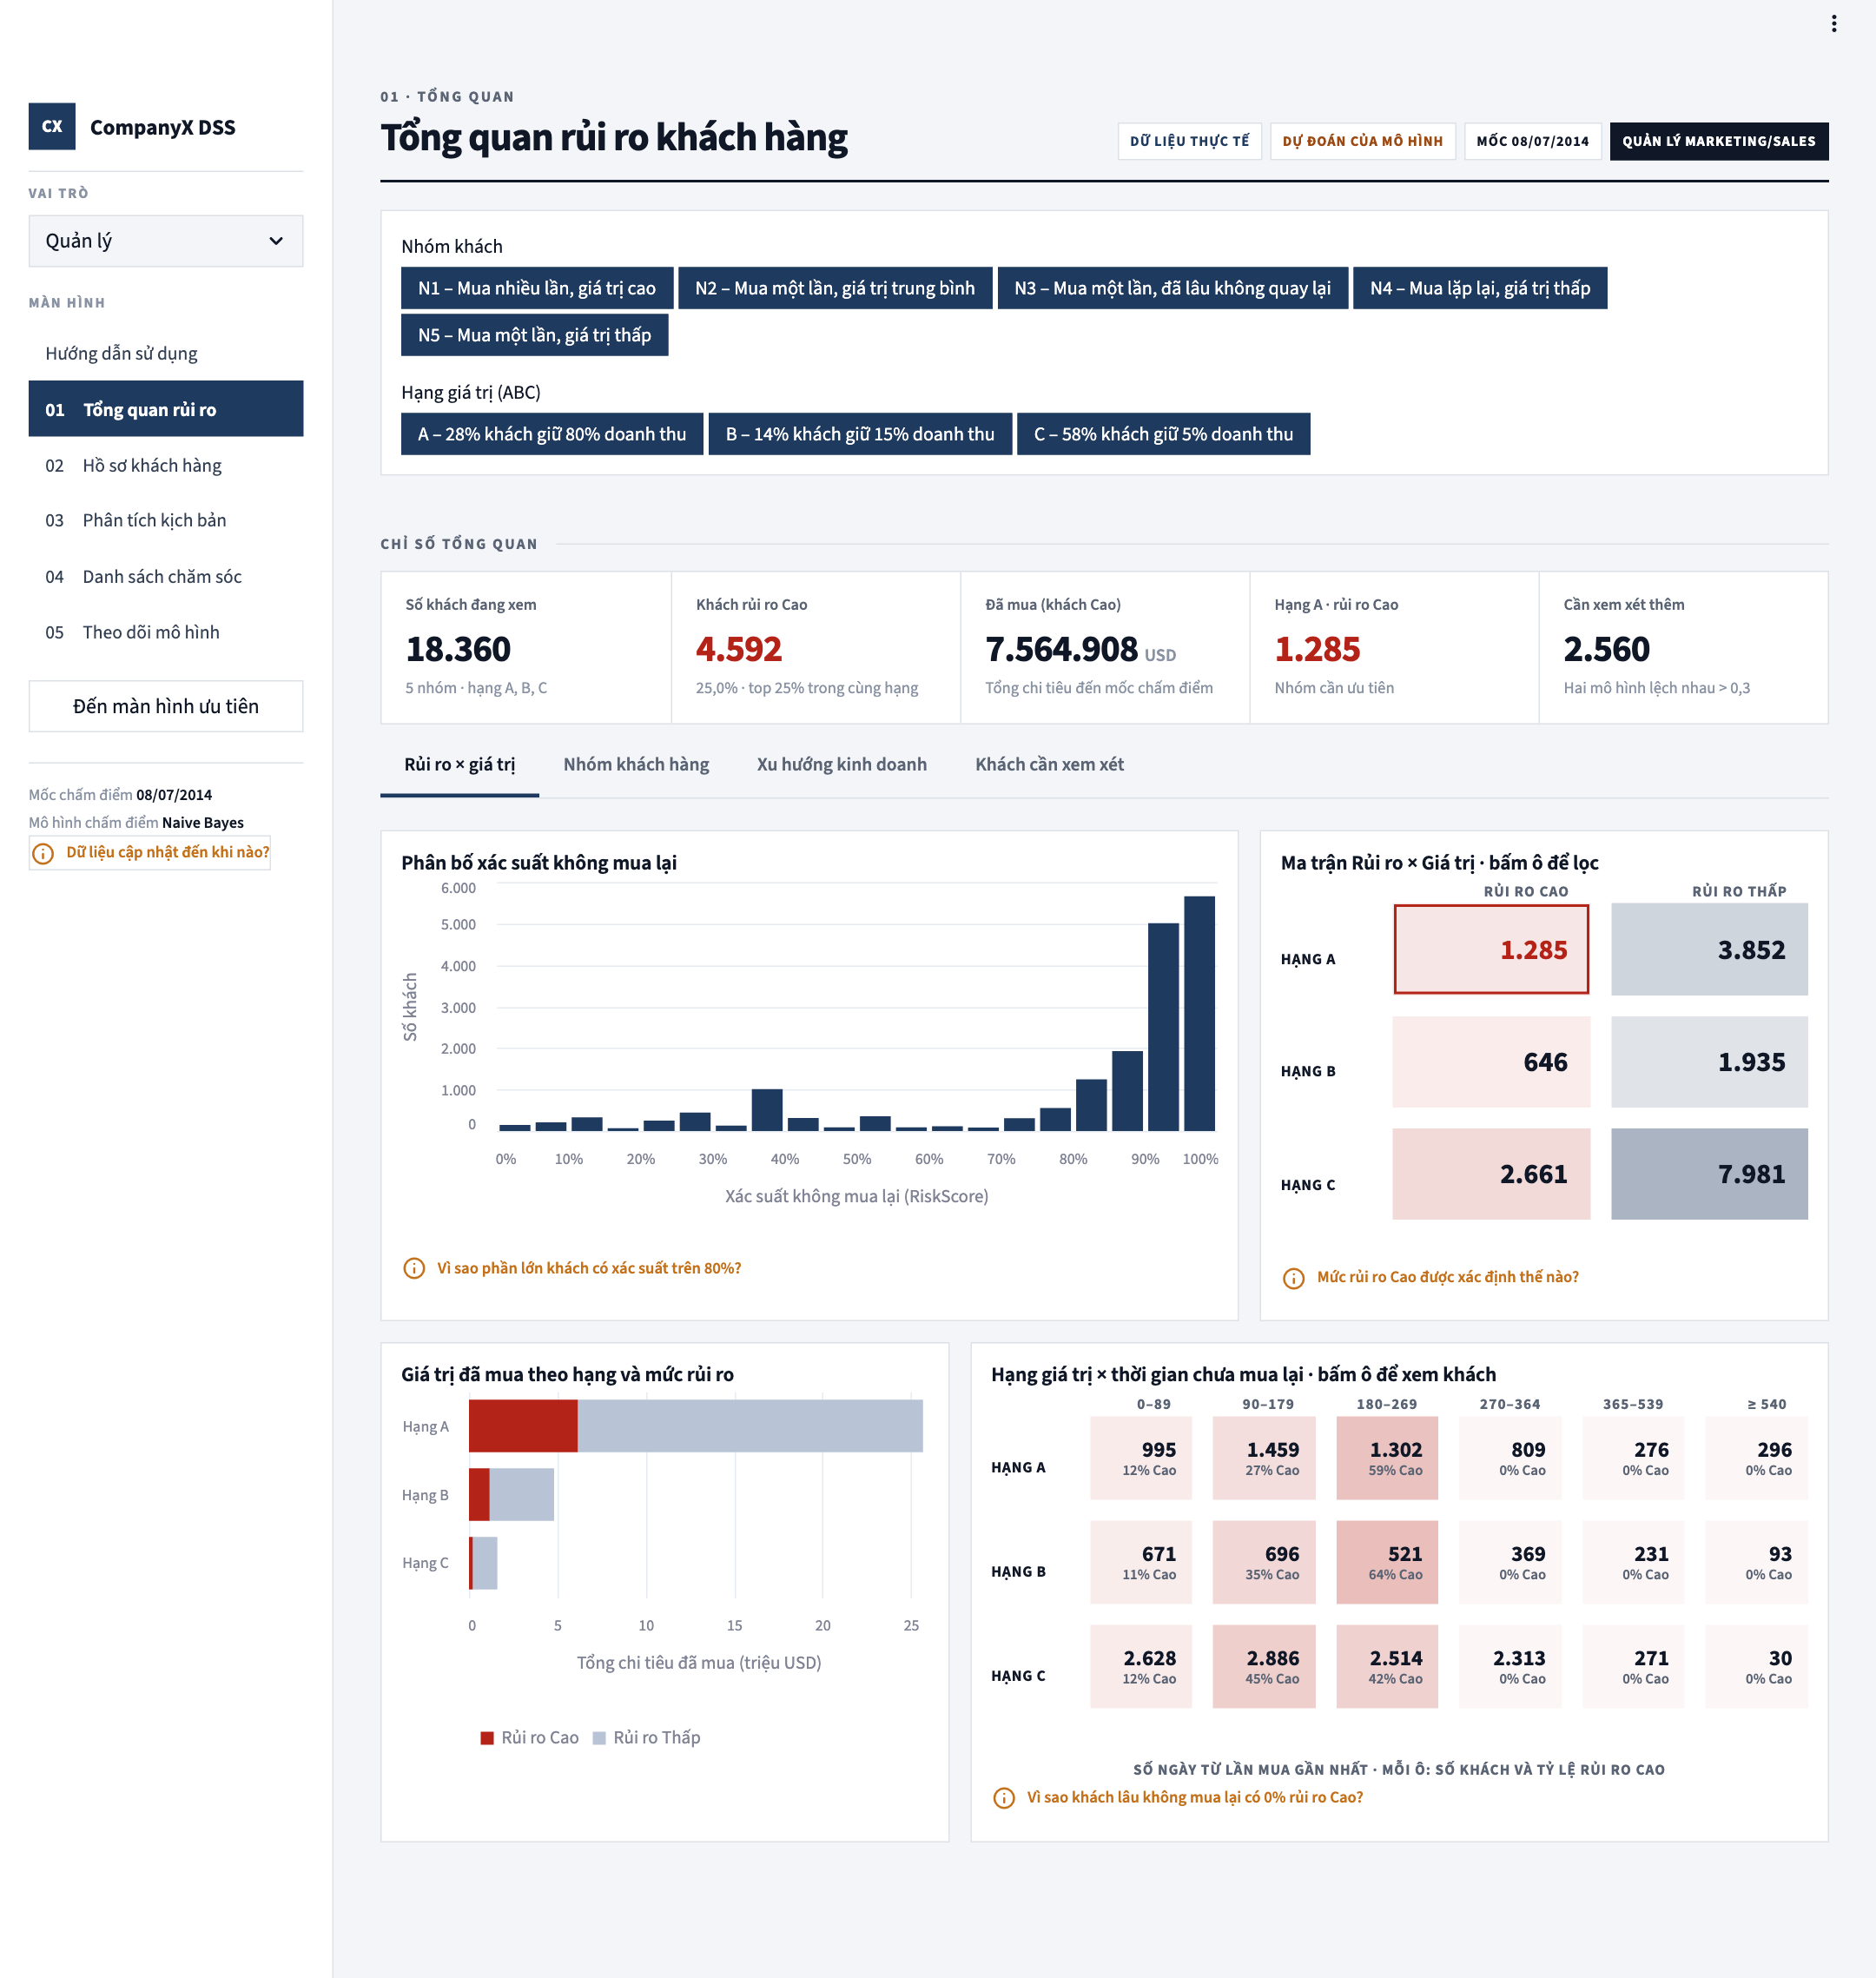
\includegraphics[width=0.95\textwidth]{d_man_hinh_1.png}
\caption{Màn hình 1: tổng quan rủi ro và phân bố khách hàng theo hạng giá trị}
\label{fig:man1}
\end{figure}

\subsection{Chăm sóc bằng cách nào: kho quy tắc}
\subsubsection{Kho quy tắc và trình tự áp dụng}
Phân hệ tri thức lưu các quy tắc IF--THEN để loại khách không đủ điều kiện, gán hình thức liên hệ, đề xuất sản phẩm và giải thích vì sao có đề xuất. Tri thức đến từ ba nguồn: từ dữ liệu (hồ sơ nhóm, cơ cấu sản phẩm, luật kết hợp), từ mô hình (\texttt{RiskScore}, \texttt{RiskLevel}, \texttt{TopFactors} là luật của lá cây mà khách rơi vào, giá trị kỳ vọng) và từ người quản lý (chính sách chăm sóc, mức ưu đãi, kênh liên hệ). Kho gồm chín quy tắc R1 đến R9 (Bảng~\ref{tab:luat}), lưu theo phiên bản tại \texttt{analytics.\allowbreak CareRule}. Bảy quy tắc đang bật. R1 và R9 cần nhật ký liên hệ và kết quả chiến dịch nên đã thiết kế nhưng còn tắt.

\begin{table}[!htbp]
\centering
\caption{Kho quy tắc chăm sóc R1 đến R9}
\label{tab:luat}
\footnotesize
\begin{tabular}{p{0.8cm}p{2.5cm}p{4.8cm}p{4.2cm}p{1.6cm}}
\toprule
Mã & Loại & Điều kiện & Hành động & Trạng thái \\
\midrule
R1 & Loại trừ & Khách đã được liên hệ trong 90 ngày trước (nhật ký CRM) & Không đưa vào danh sách mới & Tắt, thiếu dữ liệu CRM \\
R2 & Loại trừ & $p \cdot r \cdot v - c \leq 0$ & Không đưa vào danh sách chăm sóc cá nhân & Bật \\
R3 & Hình thức liên hệ & Nhóm N1 và mức rủi ro Cao & Liên hệ cá nhân kèm ưu đãi (25 USD, thành công 15\%) & Bật \\
R4 & Hình thức liên hệ & Nhóm N3 & Nội dung mời quay lại kèm ưu đãi (15 USD, thành công 12\%) & Bật \\
R5 & Hình thức liên hệ & Các trường hợp còn lại & Email cá nhân hoá gửi tự động (3 USD, thành công 5\%) & Bật \\
R6 & Sản phẩm gợi ý & Đã mua Touring Bikes, chưa mua Helmets & Gợi ý Helmets & Bật \\
R7 & Sản phẩm gợi ý & Đã mua Mountain Bikes, chưa mua Fenders & Gợi ý Fenders & Bật \\
R8 & Sản phẩm gợi ý & Đã mua Gloves chưa mua Helmets, hoặc đã mua Hydration Packs chưa mua Bottles and Cages & Gợi ý Helmets hoặc Bottles and Cages tương ứng & Bật \\
R9 & Giám sát mô hình & Đã đủ nhãn 90 ngày sau chiến dịch & So ROC-AUC với Recency trên nhóm đối chứng, cảnh báo nếu không hơn & Tắt, thiếu dữ liệu CRM \\
\bottomrule
\end{tabular}
\end{table}

Hình~\ref{fig:luongquytac} là trình tự áp dụng. Quy tắc hình thức liên hệ (R3 đến R5) chạy trước bước tối ưu: mỗi khách được gán một hình thức kèm chi phí và tỷ lệ thành công, rồi R2 và bài toán tối ưu chọn khách trong ngân sách. Quy tắc sản phẩm (R6 đến R8) chỉ áp dụng cho khách đã chọn, khách không khớp quy tắc nào nhận lời mời quay lại kèm giới thiệu chung các nhóm phụ kiện. Mỗi khuyến nghị kèm mã quy tắc đã kích hoạt, căn cứ của quy tắc và \texttt{TopFactors} của khách, và được lưu vào \texttt{analytics.\allowbreak CareRecommendation}. Người quản lý có thể thêm, sửa hoặc tắt quy tắc, mỗi thay đổi tạo một phiên bản mới có ngày hiệu lực và người cập nhật.

\begin{figure}[!htbp]
\centering
\begin{tikzpicture}[
  box/.style={draw, rounded corners=2pt, text width=10.5cm, minimum height=0.9cm, align=center, font=\small},
  off/.style={draw, dashed, rounded corners=2pt, text width=10.5cm, minimum height=0.9cm, align=center, font=\small},
  cert/.style={-{Stealth[length=2mm]}}, node distance=0.55cm]
  \node[box] (a) {Khách tại mốc chấm điểm: \texttt{RiskScore}, nhóm, hạng ABC, $v_i$};
  \node[off, below=of a] (b) {\textbf{R1} loại khách đã được liên hệ trong 90 ngày trước (cần nhật ký CRM)};
  \node[box, below=of b] (c) {\textbf{R3 đến R5} gán hình thức liên hệ kèm chi phí $c_k$ và tỷ lệ thành công $r_k$};
  \node[box, below=of c] (d) {\textbf{R2} loại khách có $EV_i \leq 0$};
  \node[box, below=of d] (e) {Tối ưu: chọn khách trong ngân sách $B$ (bài toán cái túi 0--1)};
  \node[box, below=of e] (f) {\textbf{R6 đến R8} gợi ý sản phẩm cho khách được chọn (nội dung mặc định nếu không khớp)};
  \node[box, below=of f] (g) {Danh sách chăm sóc kèm giải thích: mã quy tắc đã kích hoạt, căn cứ, \texttt{TopFactors}};
  \node[off, below=of g] (h) {\textbf{R9} giám sát mô hình sau chiến dịch (cần nhóm đối chứng và dữ liệu CRM)};
  \foreach \s/\t in {a/b,b/c,c/d,d/e,e/f,f/g}{\draw[cert] (\s) -- (\t);}
  \draw[cert, dashed] (g) -- (h);
\end{tikzpicture}

\caption{Trình tự áp dụng quy tắc và mô hình khi tạo danh sách chăm sóc}
\label{fig:luongquytac}
\end{figure}

\subsubsection{Gợi ý sản phẩm bằng luật kết hợp}
N1, N2 và N3 gần như chỉ mua xe đạp, còn N4 và N5 không mua xe và 73\% đến 77\% giá trị là phụ kiện (Bảng~\ref{tab:cocausp}). Vì vậy gợi ý cho N1 và N2 nên là phụ kiện đi kèm xe. Luật kết hợp (support, confidence và lift như ở Chương 2) tìm bằng Apriori~\cite{han2011} trên 18.360 giỏ theo khách với 17 nhóm sản phẩm nhỏ mà khách cá nhân từng mua, mỗi giỏ là tập nhóm sản phẩm khách đã mua trước mốc. Nhóm tính theo khách thay vì theo đơn vì mục đích là gợi ý món khách chưa từng mua, không phải gợi ý mua kèm tại quầy. Ngưỡng support 1\% (khoảng 184 khách) để luật có đủ số khách, confidence 20\% để cứ 5 khách mua vế trái có 1 khách mua vế phải, và lift phải lớn hơn 1. Từ 164 luật, nhóm giữ 26 luật có một mục mỗi vế và vế phải là phụ kiện hoặc quần áo. Bảng~\ref{tab:apriori} liệt kê 10 luật có lift cao nhất.

\begin{table}[!htbp]
\centering
\caption{Cơ cấu sản phẩm theo nhóm}
\label{tab:cocausp}
\footnotesize
\begin{tabular}{lrrrrr}
\toprule
Nhóm & Bikes & Accessories & Clothing & Tỷ lệ đã mua xe & NSub trung bình \\
\midrule
N1 & 98,6\% & 0,9\% & 0,5\% & 100,0\% & 3,33 \\
N2 & 96,2\% & 2,5\% & 1,3\% & 99,9\% & 2,31 \\
N3 & 100,0\% & 0,0\% & 0,0\% & 100,0\% & 1,00 \\
N4 & 0,0\% & 73,1\% & 26,9\% & 0,0\% & 3,23 \\
N5 & 0,0\% & 77,3\% & 22,7\% & 0,0\% & 1,74 \\
\bottomrule
\end{tabular}

\end{table}

\begin{table}[!htbp]
\centering
\caption{Luật kết hợp dùng làm gợi ý sản phẩm (10 trong 26 luật, xếp theo lift)}
\label{tab:apriori}
\footnotesize
\begin{tabular}{clllrr}
\toprule
Hạng & Vế trái & Vế phải & Support & Confidence & Lift \\
\midrule
1 & Shorts & Caps & 1,36\% & 24,7\% & 2,15 \\
2 & Shorts & Jerseys & 2,03\% & 36,8\% & 2,13 \\
3 & Hydration Packs & Bottles and Cages & 1,92\% & 49,9\% & 2,03 \\
4 & Mountain Bikes & Fenders & 4,85\% & 21,9\% & 1,92 \\
5 & Bike Stands & Tires and Tubes & 1,14\% & 87,5\% & 1,91 \\
6 & Caps & Jerseys & 3,70\% & 32,3\% & 1,87 \\
7 & Jerseys & Caps & 3,70\% & 21,5\% & 1,87 \\
8 & Gloves & Jerseys & 2,06\% & 27,8\% & 1,61 \\
9 & Gloves & Helmets & 3,71\% & 49,9\% & 1,55 \\
10 & Touring Bikes & Helmets & 5,69\% & 49,3\% & 1,53 \\
\bottomrule
\end{tabular}

\end{table}

Trước khi chạy Apriori, nhóm đặt năm luật ứng viên theo lý do nghiệp vụ: Touring Bikes $\rightarrow$ Helmets và Touring Bikes $\rightarrow$ Bottles and Cages (xe đường dài cần mũ và nước), Mountain Bikes $\rightarrow$ Fenders (đường bùn cần chắn bùn), Gloves $\rightarrow$ Helmets (đồ bảo hộ mua cùng nhau) và Hydration Packs $\rightarrow$ Bottles and Cages (cùng nhóm đựng nước). Cả năm đều có trong 26 luật gợi ý (Bảng~\ref{tab:apriori_dc}), bốn luật được đưa vào ba quy tắc R6, R7 và R8 (R8 gộp hai luật), luật Touring Bikes $\rightarrow$ Bottles and Cages chỉ dùng để kiểm tra, chưa đưa vào kho. Khi tính lại theo từng đơn (27.382 đơn), cả năm luật vẫn có lift lớn hơn 1, riêng Mountain Bikes $\rightarrow$ Fenders có confidence theo đơn dưới 20\% nên chỉ mạnh khi xét theo khách. Hai luật mạnh chưa dùng là Shorts $\rightarrow$ Caps và Shorts $\rightarrow$ Jerseys, có thể thêm ở phiên bản sau. Luật kết hợp chỉ mô tả các sản phẩm xuất hiện cùng nhau, không cho biết thứ tự mua hay nhân quả, nên chỉ dùng để chọn sản phẩm nêu trong nội dung chăm sóc, không dùng để chọn khách.

\begin{table}[!htbp]
\centering
\caption{Năm luật ứng viên và vị trí trong kết quả Apriori}
\label{tab:apriori_dc}
\footnotesize
\begin{tabular}{lp{4.6cm}R{1.9cm}R{1.9cm}R{2.1cm}R{1.9cm}}
\toprule
Quy tắc & Luật & Lift theo khách & Hạng trong 26 luật & Confidence theo đơn & Lift theo đơn \\
\midrule
R6 & Touring Bikes $\rightarrow$ Helmets & 1,53 & 10 & 41,2\% & 1,77 \\
R6b & Touring Bikes $\rightarrow$ Bottles and Cages & 1,47 & 12 & 25,5\% & 1,48 \\
R7 & Mountain Bikes $\rightarrow$ Fenders & 1,92 & 4 & 18,1\% & 2,35 \\
R8 & Gloves $\rightarrow$ Helmets & 1,55 & 9 & 42,0\% & 1,80 \\
R8b & Hydration Packs $\rightarrow$ Bottles and Cages & 2,03 & 3 & 45,3\% & 2,63 \\
\bottomrule
\end{tabular}

\end{table}

\subsubsection{Danh sách chăm sóc theo kênh}
Khi mỗi khách được gán một kênh $k(i)$ với chi phí $c_k$ và tỷ lệ thành công $r_k$ riêng theo R3 đến R5, bài toán thành $\max \sum_i x_i (p_i\, r_{k(i)}\, v_i - c_{k(i)})$ với ràng buộc $\sum_i x_i\, c_{k(i)} \leq B$. DSS giải bằng quy hoạch nguyên, thuật toán tham lam xếp theo lợi trên mỗi USD chi phí cho cùng lời giải. Với ngân sách 40.000 USD, DSS chọn 6.124 khách, chi 39.998 USD và đạt $Z = 256.502$ USD (Bảng~\ref{tab:theokenh}, tổng EV các dòng chênh 1 USD so với $Z$ do làm tròn), cao hơn 6,9\% so với cách xếp theo $p \cdot v$ mà bỏ qua chi phí kênh. Khi ngân sách có hạn, cách chọn đúng là xếp theo lợi trên mỗi USD chứ không phải chọn mọi khách có $EV$ dương. Kênh R4 chỉ bắt đầu có khách khi ngân sách từ khoảng 61.213 USD, nên muốn chăm sóc nhóm N3 thì phải tăng ngân sách đến mức đó. Phương án theo kênh và kịch bản cơ sở (4.000 khách, $Z$ 292.595 USD) dùng giả định chi phí và tỷ lệ thành công khác nhau nên không so trực tiếp $Z$ để kết luận phương án nào tốt hơn. Màn hình 4 (Hình~\ref{fig:man4}) trình bày danh sách này kèm nhật ký điều chỉnh và nút xuất CSV.

\begin{table}[!htbp]
\centering
\caption{Danh sách chăm sóc theo kênh}
\label{tab:theokenh}
\footnotesize
\begin{tabular}{lrrrr}
\toprule
Kênh & Khách đủ điều kiện & Được chọn & Chi phí (USD) & EV tổng (USD) \\
\midrule
R3 & 1.647 & 983 & 24.575 & 112.109 \\
R4 & 428 & 0 & 0 & 0 \\
R5 & 16.285 & 5.141 & 15.423 & 144.392 \\
Tổng & 18.360 & 6.124 & 39.998 & 256.501 \\
\bottomrule
\end{tabular}

\end{table}

\begin{figure}[!htbp]
\centering
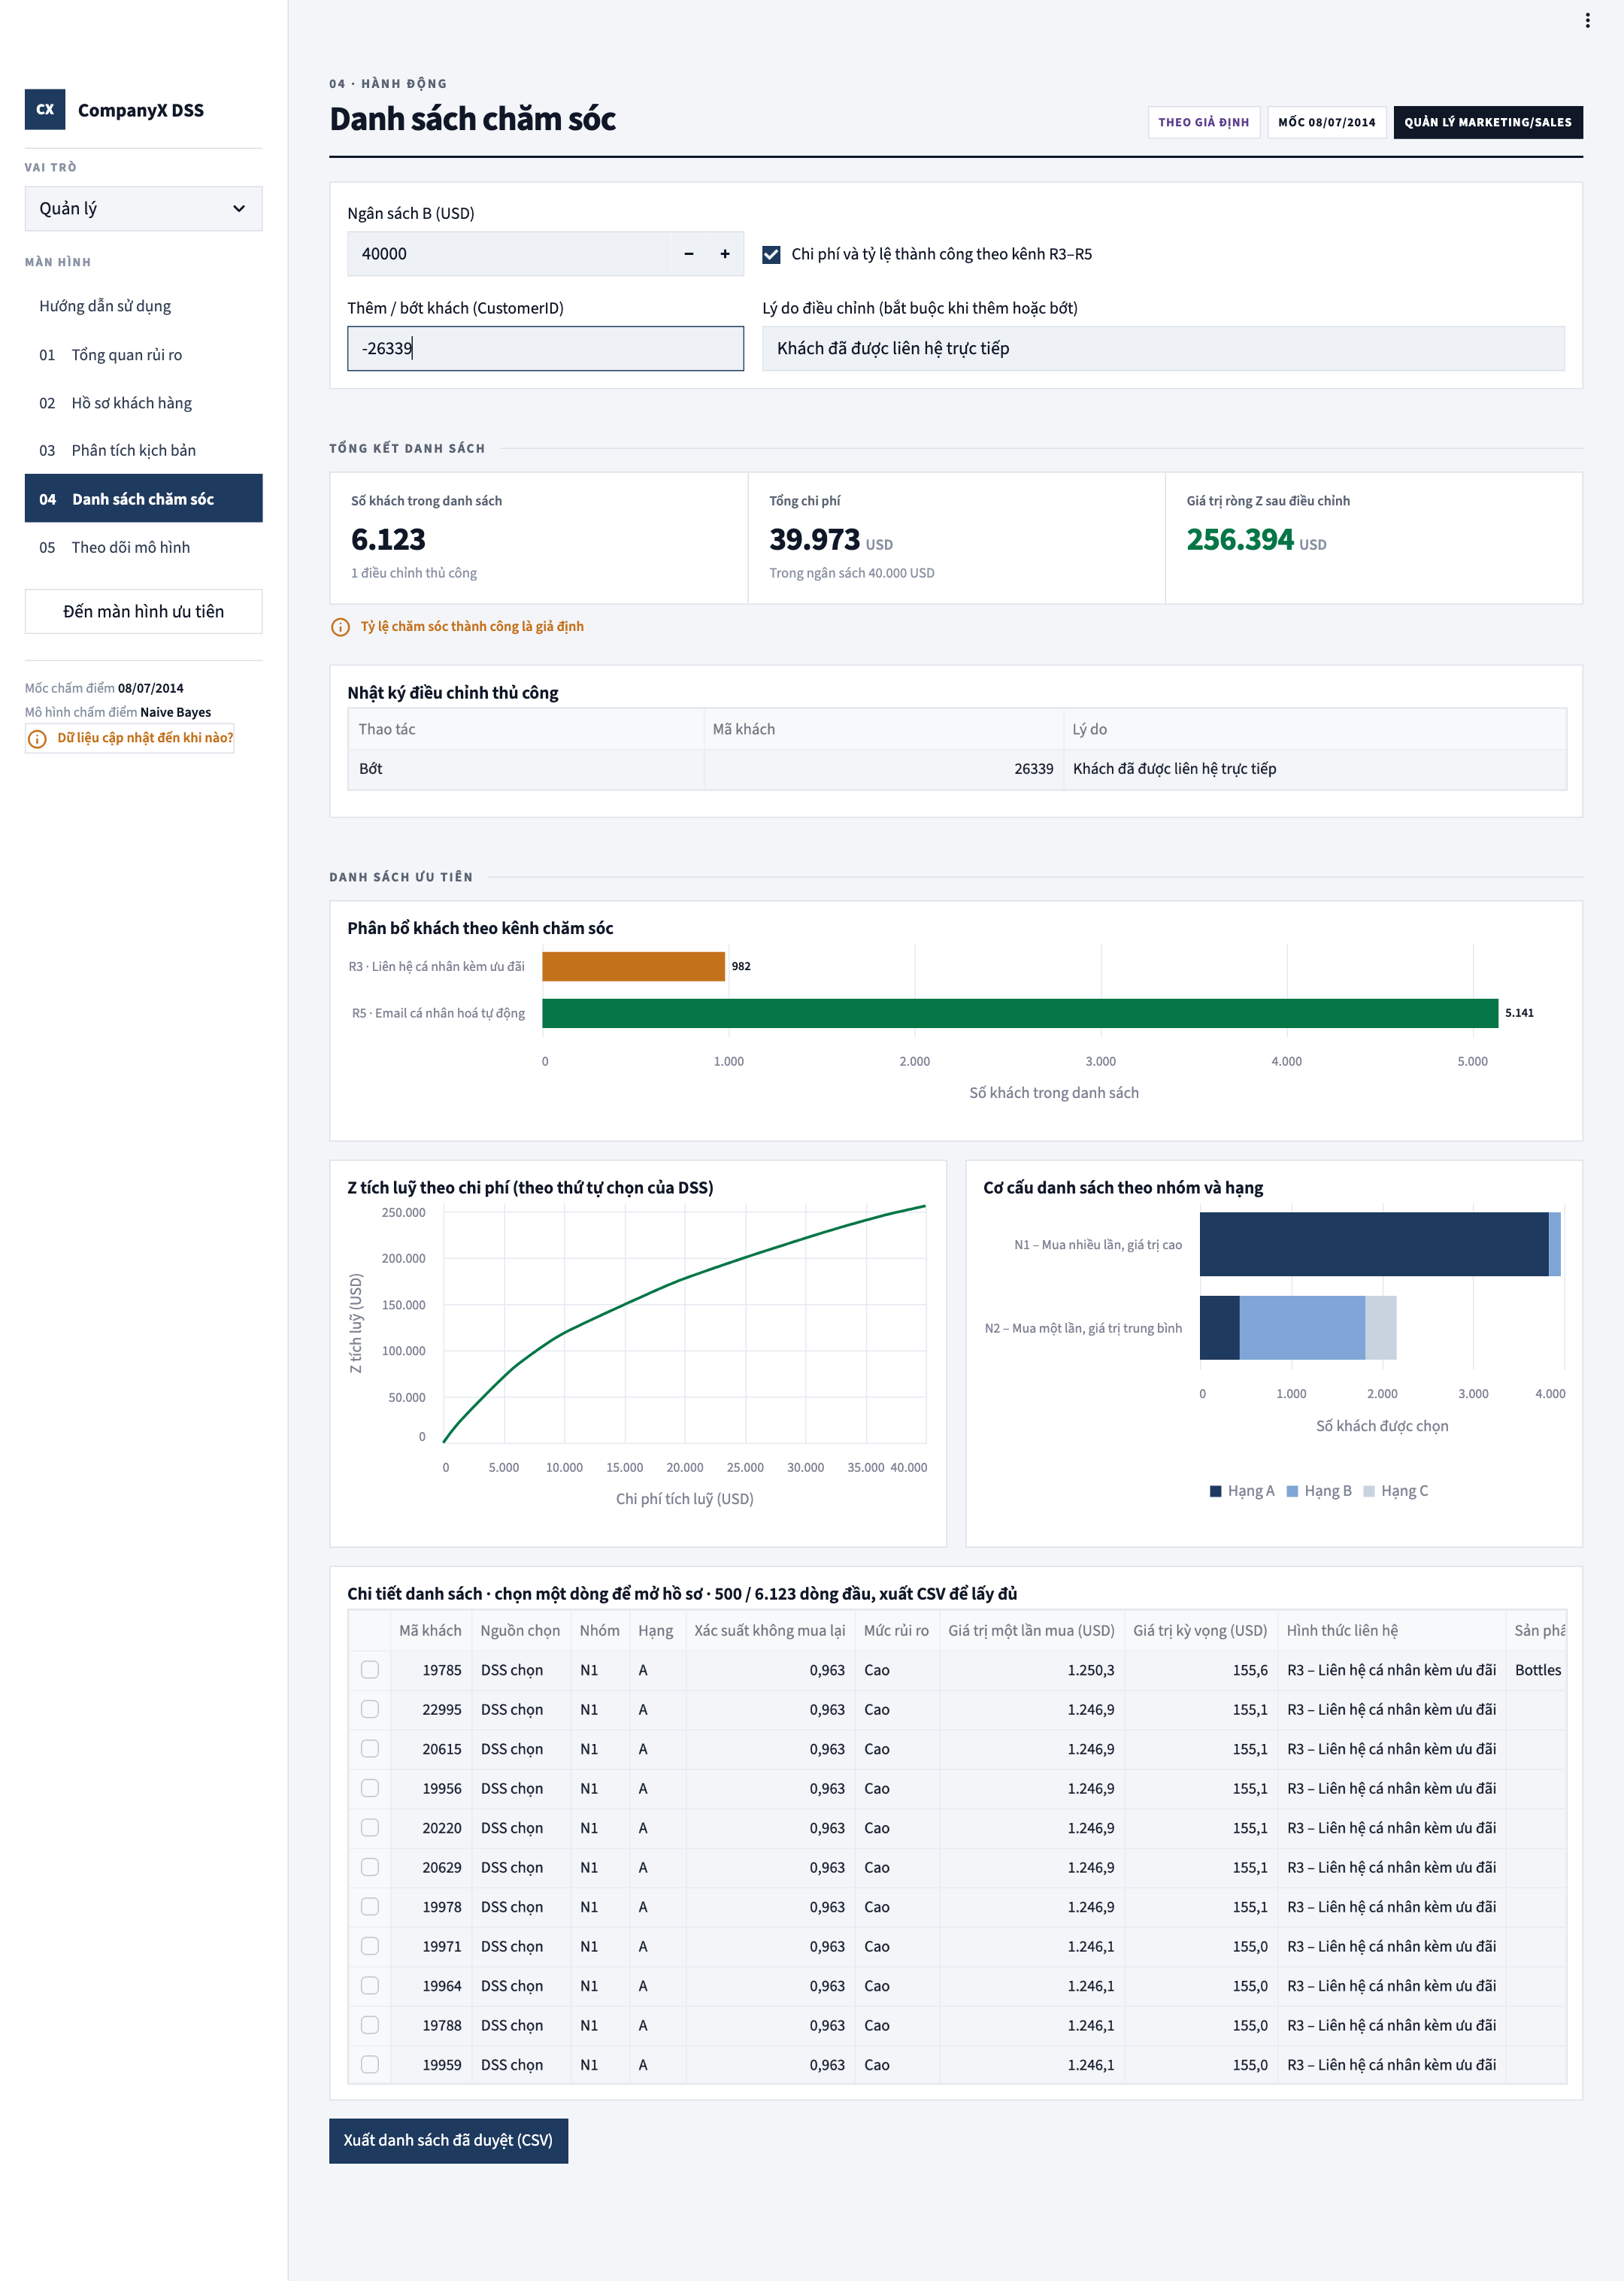
\includegraphics[width=0.95\textwidth]{d_man_hinh_4.png}
\caption{Màn hình 4: danh sách khách hàng ưu tiên chăm sóc sau khi điều chỉnh}
\label{fig:man4}
\end{figure}

\subsection{Ngân sách bao nhiêu khi chưa biết tỷ lệ thành công}
Tỷ lệ thành công $r$ chưa đo được vì chưa có chiến dịch nào. Mục này cho người quản lý thấy $Z$ phụ thuộc vào $r$ đến đâu và đặt ngân sách theo mức chấp nhận rủi ro của mình. Mọi giá trị $Z$ đều là kỳ vọng theo giả định.

\subsubsection{Độ nhạy và tìm mục tiêu}
Thay từng tham số $r$, $p$, $g$, $c$, $B$ quanh kịch bản cơ sở $\pm 20\%$ (Bảng~\ref{tab:donhay_b}, Hình~\ref{fig:donhay}). $r$ và $g$ cùng làm $Z$ đổi $\pm 22{,}7\%$ vì nhân với nhau trong doanh thu, còn $c$ và $B$ tác động ít hơn vì chỉ thêm hoặc bớt khách cuối danh sách. Trong các tham số nhân, $g$ đo được từ dữ liệu, $p$ ước lượng bằng mô hình, còn $r$ chưa có dữ liệu nên cần đo trước tiên~\cite{lemmens2020}.

\begin{table}[!htbp]
\centering
\caption{Độ nhạy của $Z$ khi từng tham số thay đổi 20\%}
\label{tab:donhay_b}
\footnotesize
\resizebox{\textwidth}{!}{\begin{tabular}{lrrrr}
\toprule
Tham số & $Z$ khi giảm 20\% (USD) & Chênh & $Z$ khi tăng 20\% (USD) & Chênh \\
\midrule
$r$ & 226.076 & $-$22,7\% & 359.114 & +22,7\% \\
$p$ & 226.076 & $-$22,7\% & 327.591 & +12,0\% \\
$g$ (qua $v$) & 226.076 & $-$22,7\% & 359.114 & +22,7\% \\
$c$ & 342.856 & +17,2\% & 251.887 & $-$13,9\% \\
$B$ & 251.405 & $-$14,1\% & 326.198 & +11,5\% \\
\bottomrule
\end{tabular}
}
\end{table}

\begin{figure}[!htbp]
\centering
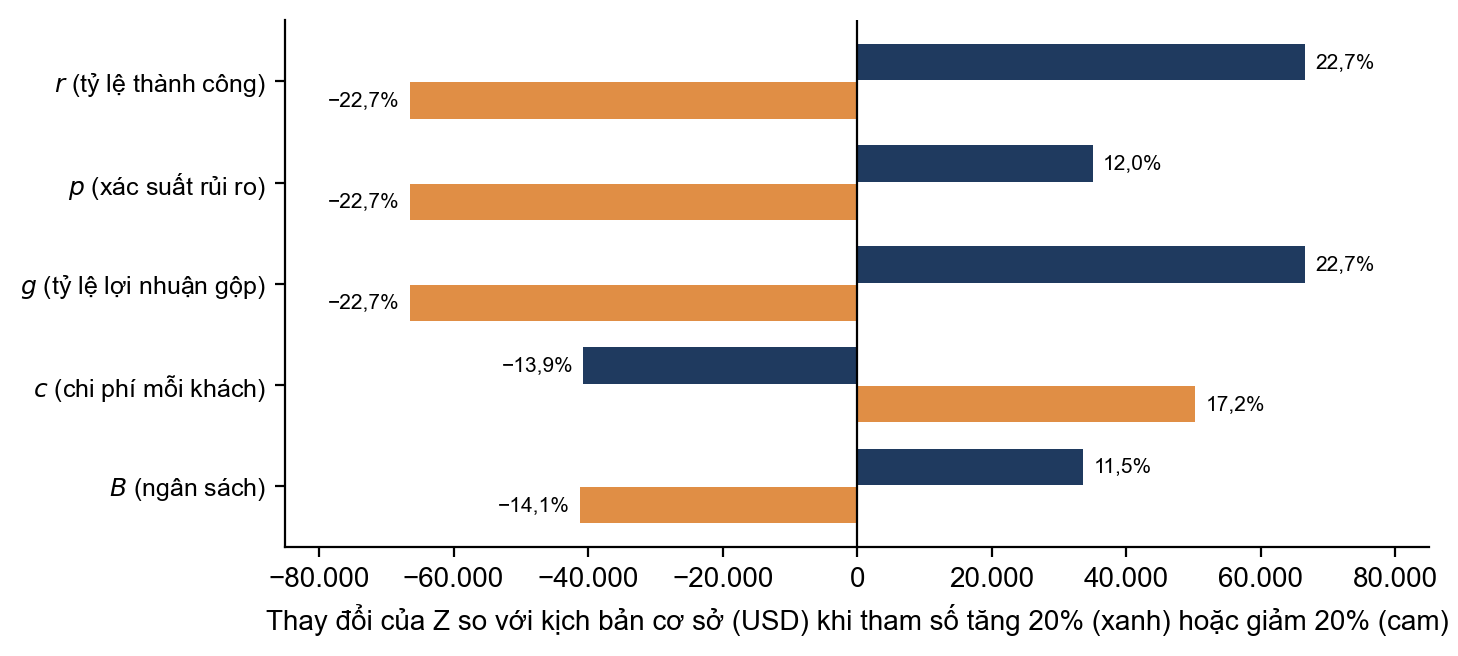
\includegraphics[width=0.8\textwidth]{d_do_nhay.png}
\caption{Thay đổi của $Z$ khi từng tham số của kịch bản cơ sở tăng hoặc giảm 20\%}
\label{fig:donhay}
\end{figure}

Tìm mục tiêu trả lời câu hỏi ngược: $r$ phải bằng bao nhiêu để $Z$ đạt mức $Z^*$. Với danh sách $K$ khách đã chốt, $Z$ là hàm bậc nhất của $r$ nên
\begin{equation}
    r^* = \frac{Z^* + c\,K}{\sum_{i=1}^{K} p_i\, v_i} \label{eq:rstar}
\end{equation}
Mức $r$ hoà vốn ($Z^*=0$) là 1,20\%, mức để $Z$ đạt 100.000 USD là 4,21\%. Chiến dịch chỉ lỗ khi tỷ lệ thành công thật dưới khoảng 1,2\%.

\subsubsection{Ba tiêu chí ra quyết định và mô phỏng}
Khi $r$ chưa biết, phương án là mức ngân sách $B$ và trạng thái là ba mức $r$: 2\% (bi quan), 10\% (cơ sở) và 20\% (lạc quan) với xác suất giả định 30\%, 50\% và 20\%. Gọi $Z(B,s)$ là giá trị ròng của phương án $B$ ở trạng thái $s$, ba tiêu chí ở Chương 2 là:
\begin{align}
    \text{Lạc quan:}\quad & B^* = \arg\max_B \left[\max_s Z(B,s)\right] \label{eq:lacquan}\\
    \text{Bi quan:}\quad & B^* = \arg\max_B \left[\min_s Z(B,s)\right] \label{eq:biquan}\\
    \text{Giá trị kỳ vọng:}\quad & B^* = \arg\max_B \sum_s P(s)\, Z(B,s) \label{eq:kyvong}
\end{align}
Bảng~\ref{tab:payoff} là $Z$ theo ngân sách và $r$. Người lạc quan và tiêu chí giá trị kỳ vọng chọn $B = 100.000$ USD, người bi quan chọn $B = 40.000$ USD. DSS không chọn thay người quản lý mà đưa ra phương án cho từng phong cách ra quyết định.

\begin{table}[!htbp]
\centering
\caption{$Z$ theo ngân sách và tỷ lệ chăm sóc thành công (USD)}
\label{tab:payoff}
\footnotesize
\resizebox{\textwidth}{!}{\begin{tabular}{rrrrrr}
\toprule
Ngân sách $B$ (USD) & Số khách & $r=2\%$ & $r=10\%$ & $r=20\%$ & Giá trị kỳ vọng \\
\midrule
20.000 & 2.000 & 18.413 & 172.066 & 364.132 & 164.383 \\
40.000 & 4.000 & 26.519 & 292.595 & 625.189 & 279.291 \\
60.000 & 6.000 & 23.878 & 359.388 & 778.775 & 342.612 \\
100.000 & 8.554 & 8.815 & 386.235 & 858.009 & 367.364 \\
\bottomrule
\end{tabular}
}
\end{table}

Thay cho ba mức rời rạc, mô phỏng coi $r$ là đại lượng ngẫu nhiên theo phân phối Beta (phân phối cho đại lượng từ 0 đến 1) với $\alpha=2{,}2$, $\beta=19{,}8$, trung bình 10\%, các $r_k$ theo kênh co giãn cùng hệ số. Mỗi lần mô phỏng rút một giá trị $r$ rồi tính $Z$ cho danh sách đã chốt, lặp 10.000 lần~\cite{turban2011}. Mô hình được kiểm định bằng cách tại $r=10\%$ kết quả phải trùng kịch bản cơ sở. Kết quả (Hình~\ref{fig:mophong}): $r$ trung bình 9,9\%, $Z$ trung bình 290.490 USD và xác suất lỗ 1,7\%. Xác suất này đúng theo phân phối giả định, không phải xác suất lỗ đã xác thực.

\begin{figure}[!htbp]
\centering
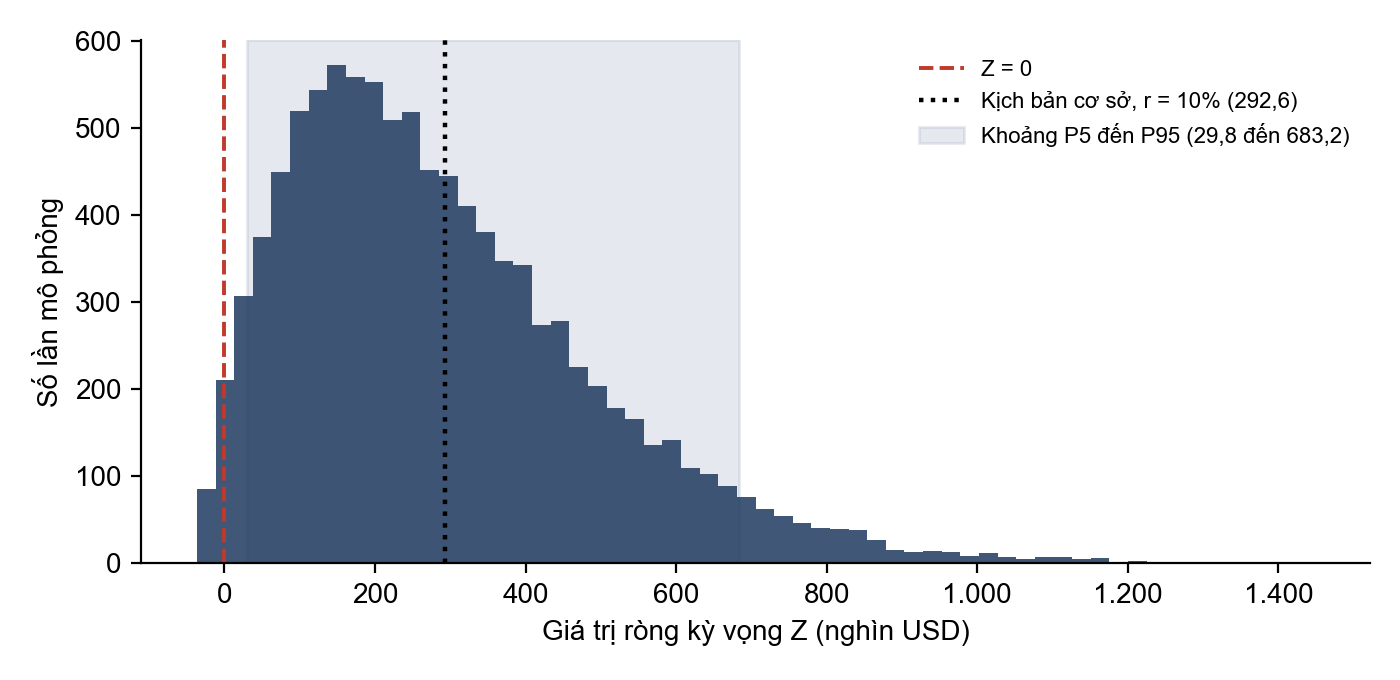
\includegraphics[width=0.7\textwidth]{d_mo_phong.png}
\caption{Phân bố của $Z$ trong 10.000 lần mô phỏng với $r$ theo phân phối Beta}
\label{fig:mophong}
\end{figure}

\subsubsection{Dự báo theo tháng}
Để ước quy mô kỳ 90 ngày khi đặt ngân sách và để cảnh báo khi thực tế lệch xa dự báo, màn hình theo dõi (Hình~\ref{fig:man5}) dùng hồi quy tuyến tính~\cite{han2011} trên chuỗi tháng của số đơn và doanh thu, với biến xu hướng và biến chỉ thị tháng. MAPE (sai số phần trăm tuyệt đối trung bình) ở hai tháng ngoài mẫu (tháng 4 và 5/2014) là 8,2\% với số đơn và 15,4\% với doanh thu, tốt hơn nhiều so với mức nền cùng tháng năm trước (84,9\% và 70,1\%) (Bảng~\ref{tab:dubao}). Tháng 6/2014 lệch mạnh vì không có đơn xe đạp, đúng là tình huống bất thường mà chức năng này cần phát hiện.

\begin{table}[!htbp]
\centering
\caption{Dự báo hồi quy tuyến tính số đơn và doanh thu}
\label{tab:dubao}
\footnotesize
\resizebox{\textwidth}{!}{\begin{tabular}{lrrr}
\toprule
Chỉ số & MAPE tháng 4--5/2014 & MAPE mức nền (cùng tháng năm trước) & Dự báo vượt thực tế tháng 6/2014 \\
\midrule
Số đơn & 8,2\% & 84,9\% & 134\% \\
Doanh thu & 15,4\% & 70,1\% & 3.721\% \\
\bottomrule
\end{tabular}
}
\end{table}

\begin{figure}[!htbp]
\centering
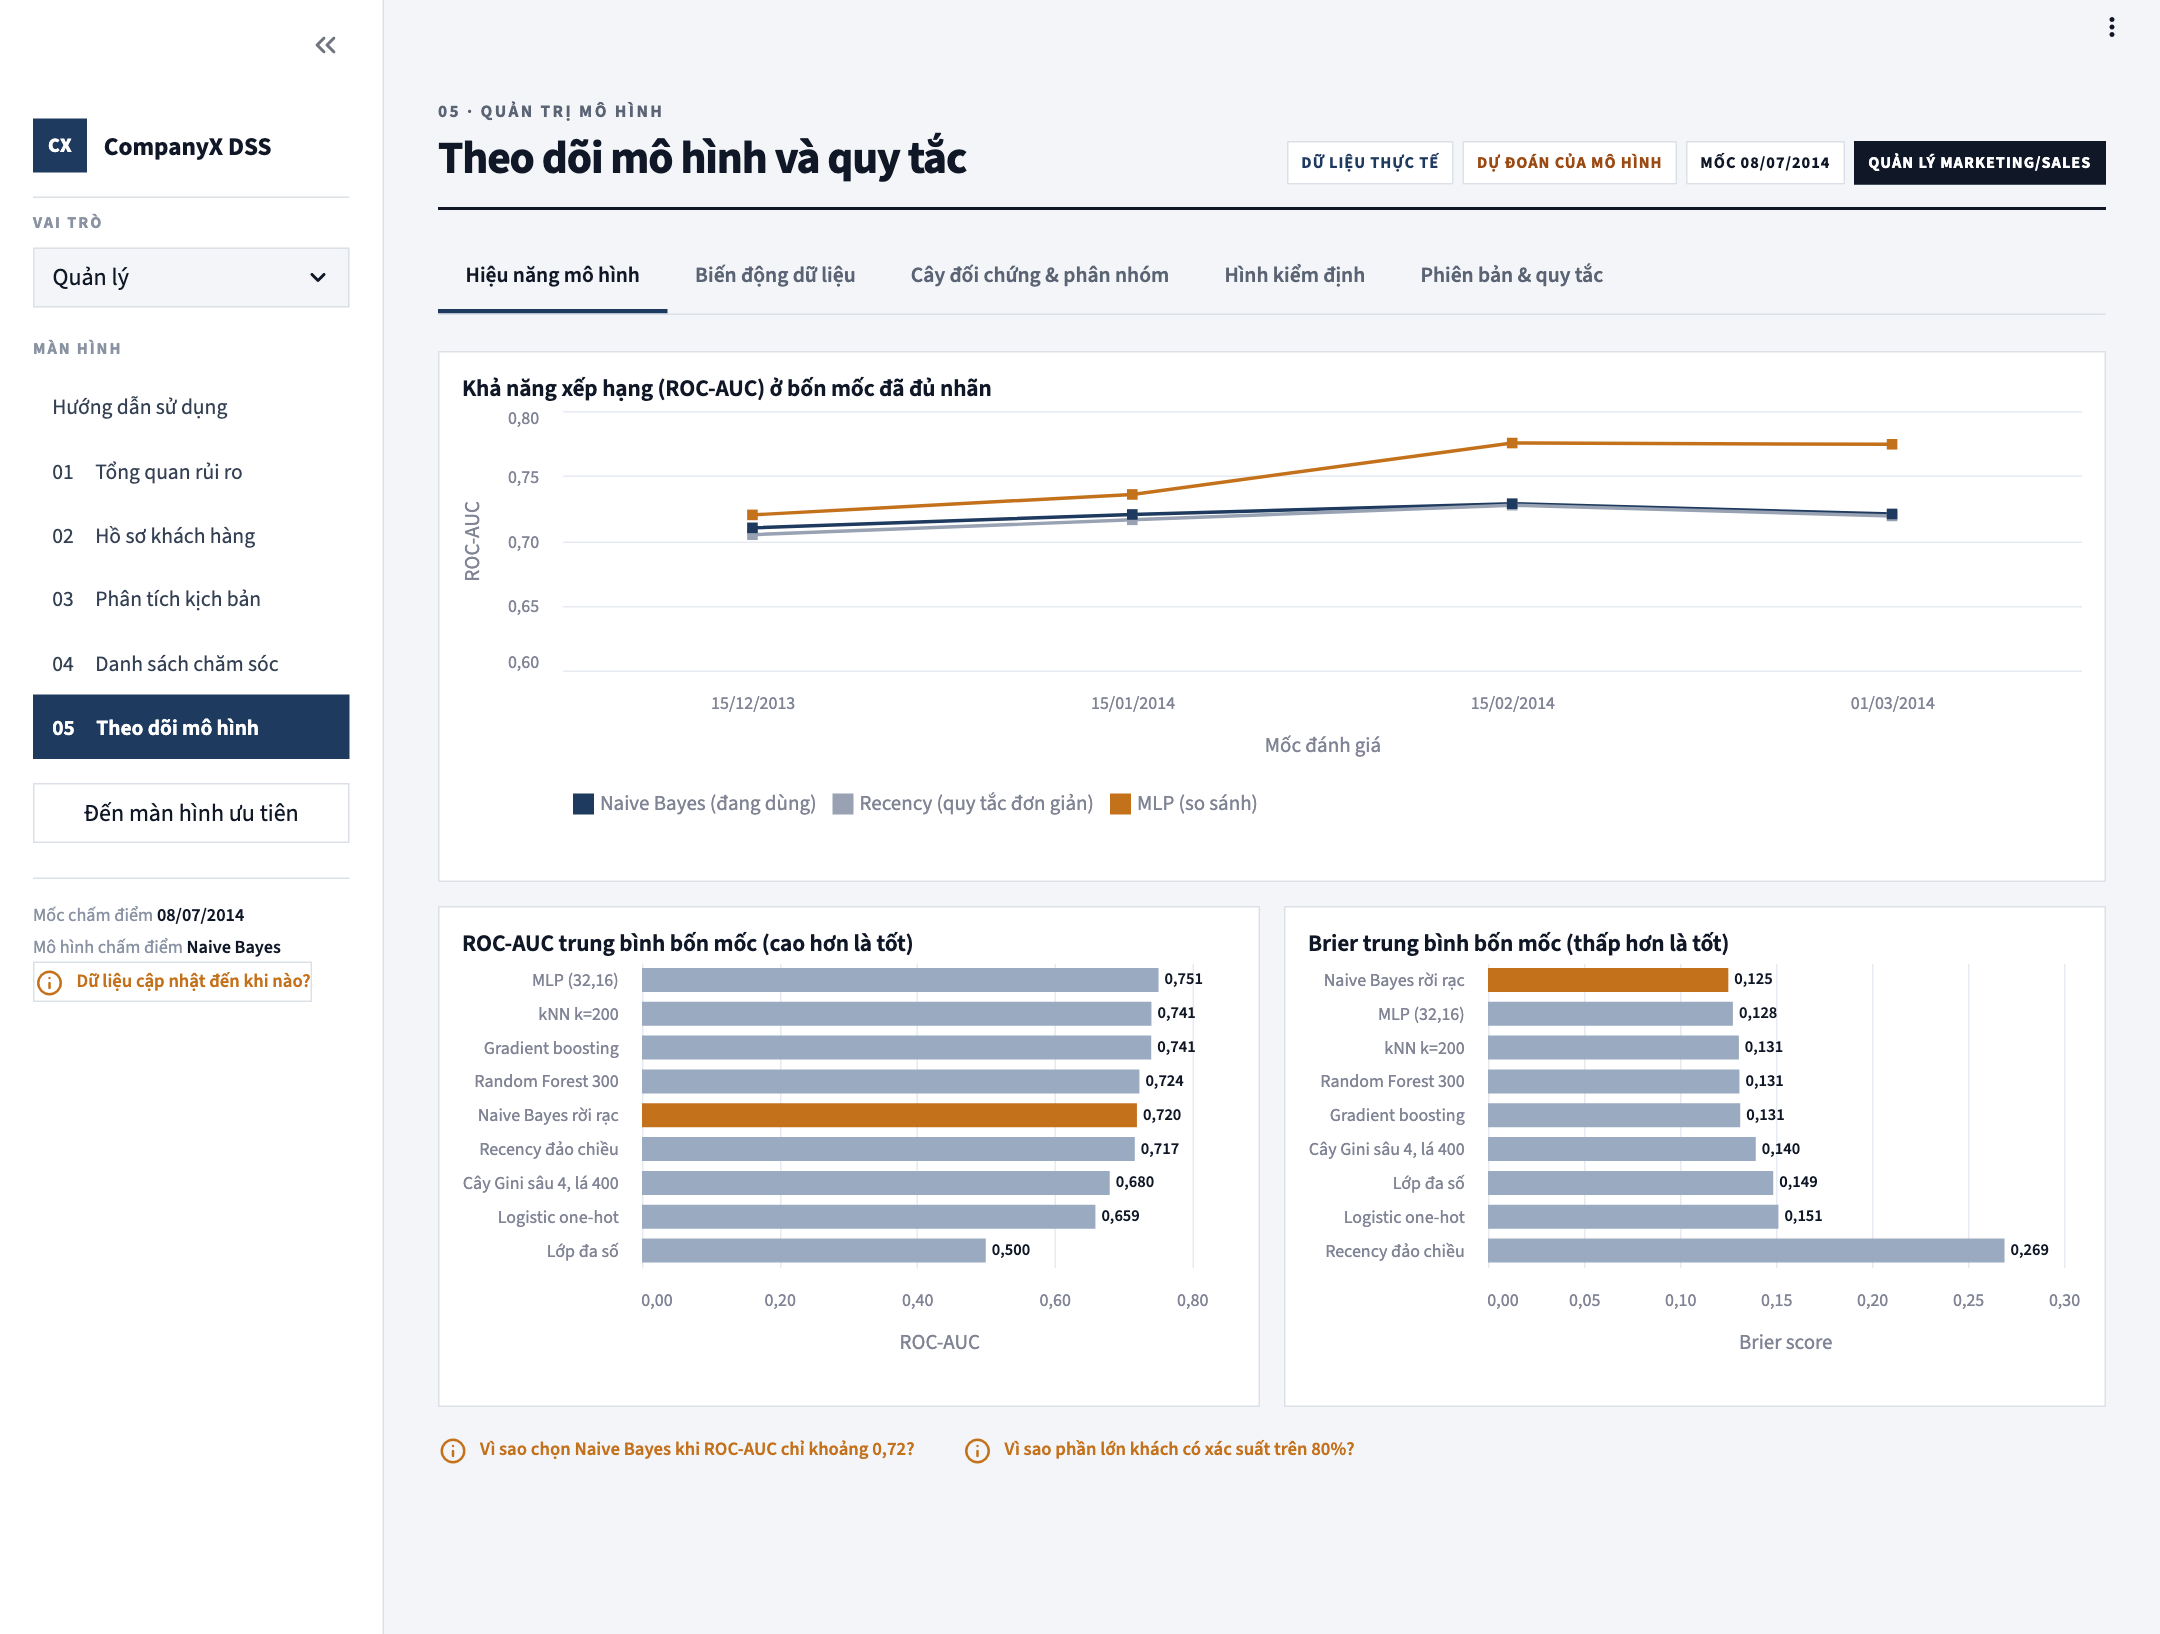
\includegraphics[width=0.95\textwidth]{d_man_hinh_5.png}
\caption{Màn hình 5: theo dõi mô hình và quy tắc, thẻ hiệu năng mô hình}
\label{fig:man5}
\end{figure}

\subsection{Hiện thực DSS: giao diện và demo}
\subsubsection{Người dùng, vai trò và màn hình}\label{sec:vaitro}
Phân hệ giao diện nhận lệnh và tham số của người dùng, chuyển cho ba phân hệ dữ liệu, mô hình và tri thức, rồi trình bày kết quả~\cite{turban2011} (Hình~\ref{fig:uims}). Giao diện là ứng dụng web Streamlit gồm năm màn hình (Bảng~\ref{tab:manhinh}) đi theo bốn pha ở Bảng~\ref{tab:quytrinh}, nhưng người dùng mở được màn hình theo thứ tự bất kỳ. Thao tác kiểu OLAP (roll-up, drill-down, slice và dice) thực hiện bằng truy vấn tổng hợp trên kho~\cite{kimball2013}, không dùng máy chủ OLAP riêng. Xác suất và tỷ lệ khách rủi ro cao không cộng dồn được (gộp hai nhóm thì phải tính lại tỷ lệ trên tổng số khách, không cộng hai tỷ lệ), nên khi gộp lên mức cao hơn hệ thống tính lại trên số khách phân biệt trong cùng một mốc. Mỗi con số trên màn hình có nhãn cho biết là dữ liệu thực tế, dự đoán của mô hình hay theo giả định, kèm ngày chấm điểm và phiên bản mô hình. Khi người quản lý thêm hoặc bớt khách, hệ thống tính lại chi phí và $Z$, kiểm tra ràng buộc ngân sách và quy tắc R2. Hình~\ref{fig:man2} minh hoạ màn hình 2 với hồ sơ khách 26339.

\begin{figure}[!htbp]
\centering
\begin{tikzpicture}[
  box/.style={draw, rounded corners=2pt, align=center, font=\small, minimum height=0.9cm},
  cert/.style={-{Stealth[length=2mm]}}]
  \node[box, text width=2.2cm, minimum height=2.2cm] (u) at (0,0) {Người dùng};
  \node[box, text width=3.0cm, minimum height=2.2cm] (m) at (5.2,0) {Phân hệ giao diện\\(quản lý hội thoại)};
  \node[box, text width=2.8cm] (d) at (10.6,1.4) {Phân hệ dữ liệu};
  \node[box, text width=2.8cm] (mo) at (10.6,0) {Phân hệ mô hình};
  \node[box, text width=2.8cm] (t) at (10.6,-1.4) {Phân hệ tri thức};
  \draw[cert] ([yshift=0.45cm]u.east) -- node[above, font=\scriptsize, text width=2.6cm, align=center] {ngôn ngữ hành động: chọn mốc, lọc, nhập tham số, duyệt} ([yshift=0.45cm]m.west);
  \draw[cert] ([yshift=-0.45cm]m.west) -- node[below, font=\scriptsize, text width=2.6cm, align=center] {ngôn ngữ hiển thị: thẻ chỉ số, biểu đồ, bảng, danh sách} ([yshift=-0.45cm]u.east);
  \draw[cert, <->, {Stealth[length=2mm]}-{Stealth[length=2mm]}] (m.east) -- (d.west);
  \draw[{Stealth[length=2mm]}-{Stealth[length=2mm]}] (m.east) -- (mo.west);
  \draw[{Stealth[length=2mm]}-{Stealth[length=2mm]}] (m.east) -- (t.west);
\end{tikzpicture}

\caption{Kiến trúc phân hệ giao diện người dùng của DSS}
\label{fig:uims}
\end{figure}

\begin{table}[!htbp]
\centering
\caption{Năm màn hình của CompanyX DSS}
\label{tab:manhinh}
\footnotesize
\begin{tabular}{p{0.6cm}p{2.8cm}p{9.2cm}p{1.8cm}}
\toprule
STT & Màn hình & Chức năng chính & Pha \\
\midrule
1 & Tổng quan rủi ro & Chọn mốc, lọc theo nhóm và hạng ABC, xem số khách, tỷ lệ khách mức Cao, phân bố xác suất, ma trận Rủi ro $\times$ Giá trị, cơ cấu năm nhóm, xu hướng kinh doanh và khách cần xem xét & Tìm hiểu \\
2 & Hồ sơ khách hàng & Tìm theo mã khách, xem RFM, lịch sử mua, \texttt{RiskScore} và \texttt{TreeScore}, luật của lá và cờ lệch giữa hai mô hình, nhóm, hạng, khuyến nghị và quy tắc đã kích hoạt & Tìm hiểu, lựa chọn \\
3 & Phân tích kịch bản & Ba thanh trượt $r$, $c$, $B$, bốn chỉ số kết quả ($Z$, số khách, chi phí, số khách giữ lại kỳ vọng), đường $Z$ theo ngân sách, lưu và so sánh kịch bản, độ nhạy, tìm mục tiêu, $Z$ theo ngân sách khi chưa biết $r$, mô phỏng, theo kênh & Thiết kế, lựa chọn \\
4 & Danh sách chăm sóc & Ngân sách và tuỳ chọn chi phí theo kênh, thêm hoặc bớt khách (bắt buộc ghi lý do), nhật ký điều chỉnh, $Z$ tích luỹ theo chi phí, bảng chi tiết giải thích vì sao khách được chọn, xuất CSV & Lựa chọn, thực hiện \\
5 & Theo dõi mô hình và quy tắc & ROC-AUC và Brier ở các mốc đã đủ nhãn so với quy tắc Recency, biến động cơ cấu khách, cây đối chứng và phân nhóm, phiên bản mô hình và quy tắc, đề xuất quy tắc mới (chờ duyệt) & Thực hiện \\
\bottomrule
\end{tabular}
\end{table}

\begin{figure}[!htbp]
\centering
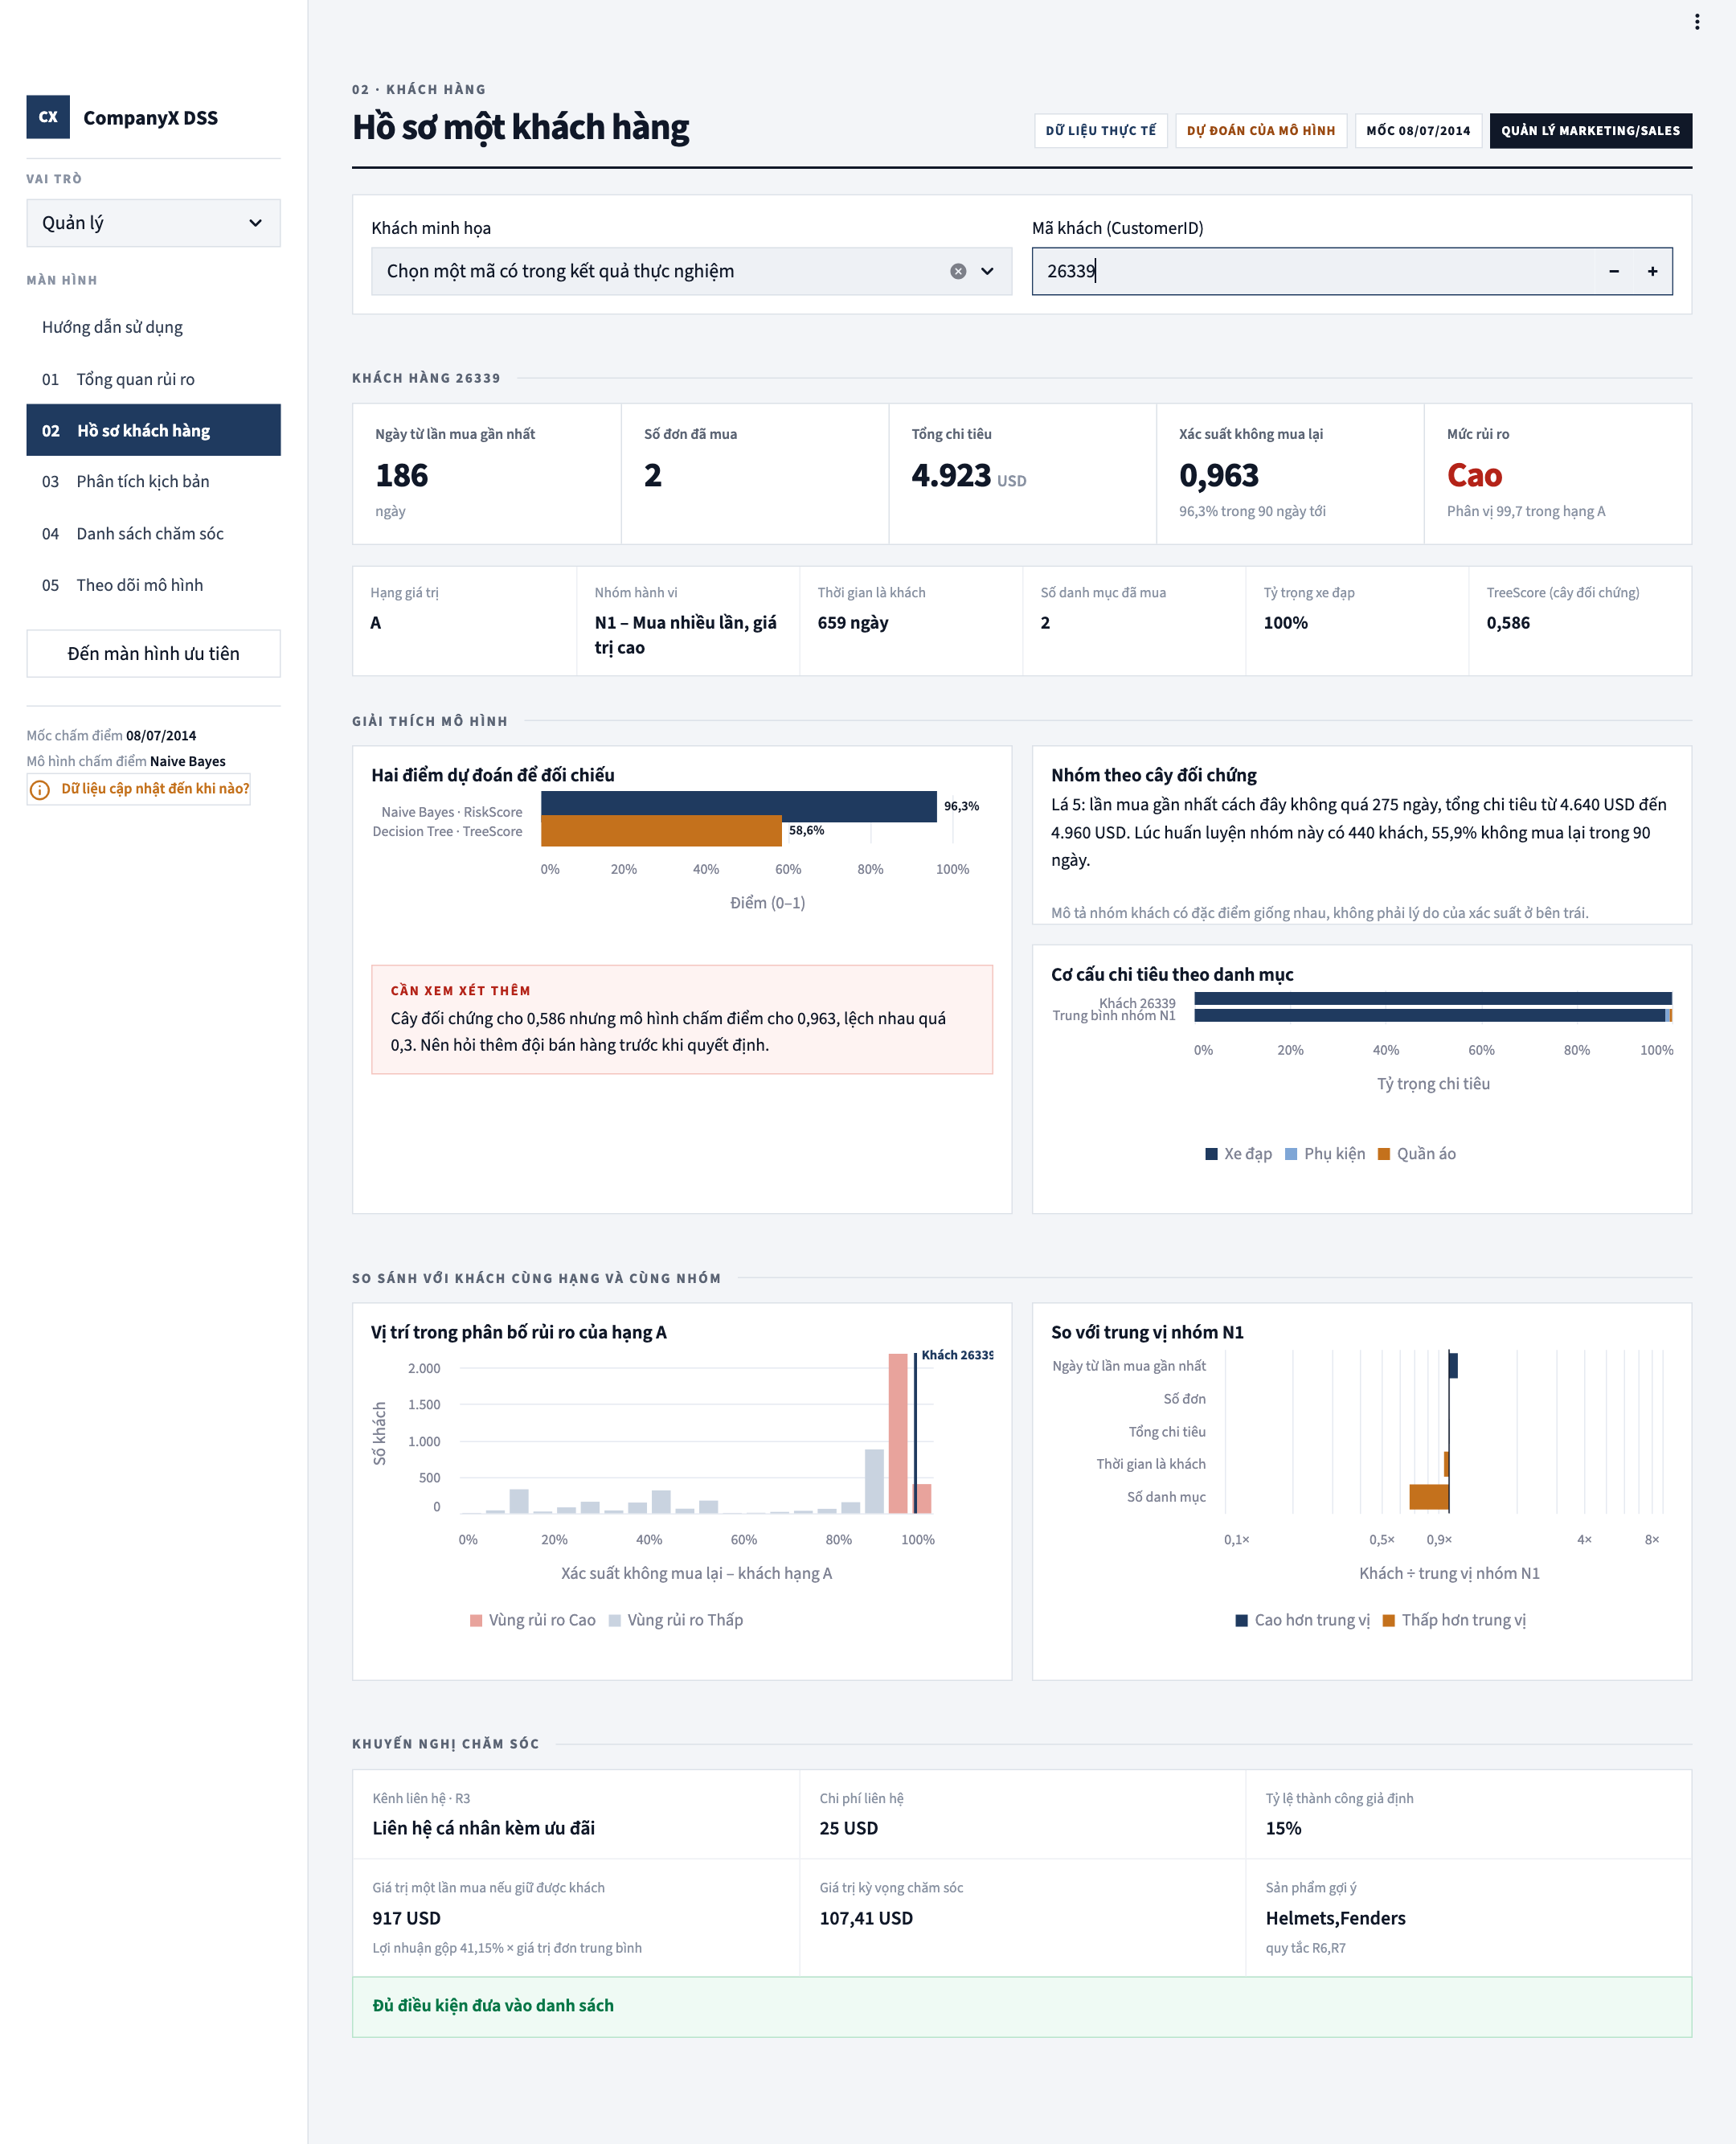
\includegraphics[width=0.95\textwidth]{d_man_hinh_2.png}
\caption{Màn hình 2: tra cứu hồ sơ và đối chiếu kết quả dự đoán của khách hàng 26339}
\label{fig:man2}
\end{figure}

Giao diện phân quyền theo ba nhóm người dùng (Bảng~\ref{tab:quyen}). Bản demo hiện thực một phần: cả ba vai trò mở được cả năm màn hình, khác nhau ở màn hình mở đầu và ở hai chức năng xuất danh sách và đề xuất quy tắc. Bản demo chưa có đăng nhập, vai trò chọn ở thanh bên chỉ để minh hoạ. Đề tài chỉ dùng giao diện đồ hoạ trên web, chưa có bộ xử lý ngôn ngữ tự nhiên như kiến trúc đầy đủ trong~\cite{turban2011}.

\begin{table}[!htbp]
\centering
\caption{Ba nhóm người dùng: quyền hạn theo thiết kế và phần đã hiện thực trong demo}
\label{tab:quyen}
\footnotesize
\begin{tabular}{p{3.0cm}p{5.4cm}p{6.0cm}}
\toprule
Người dùng & Quyền hạn theo thiết kế & Trong bản demo \\
\midrule
Quản lý Marketing/Sales & Xem, chạy kịch bản, duyệt danh sách, phê duyệt quy tắc mới hoặc sửa đổi & Mở đầu ở màn hình 1. Xuất CSV danh sách đã duyệt, đề xuất quy tắc mới (chờ duyệt) \\
Nhân viên phân tích dữ liệu & Xem, chạy chấm điểm, tạo và sửa quy tắc ở trạng thái chờ duyệt, không duyệt danh sách & Mở đầu ở màn hình 5. Chỉ xem danh sách, không có nút xuất CSV. Đề xuất quy tắc mới \\
Nhân viên chăm sóc khách hàng & Xem danh sách đã duyệt, xuất CSV, cập nhật kết quả liên hệ & Mở đầu ở màn hình 4. Xuất CSV để liên hệ khách. Không thấy mục đề xuất quy tắc \\
\bottomrule
\end{tabular}
\end{table}

\subsubsection{Công nghệ và tích hợp}\label{sec:congnghe}
Bảng~\ref{tab:congnghe} nêu các thành phần công nghệ của bản hiện thực và việc mỗi thành phần đảm nhiệm.

\begin{table}[!htbp]
\centering
\caption{Thành phần công nghệ của CompanyX DSS}
\label{tab:congnghe}
\footnotesize
\begin{tabular}{p{3.3cm}p{4.2cm}p{7.2cm}}
\toprule
Thành phần & Công nghệ & Việc đảm nhiệm \\
\midrule
Kho dữ liệu & SQL Server, CSDL \texttt{CompanyX\_DW} & Lưu các bảng của kho và các bảng \texttt{analytics} (điểm rủi ro, phân nhóm, đăng ký mô hình, quy tắc chăm sóc) \\
Mô hình và phân tích & Python, scikit-learn, scipy & Học Naive Bayes và cây, chấm điểm và sinh tệp SQL để ghi điểm vào kho, giải bài toán chọn khách bằng quy hoạch nguyên \\
Kết nối & pyodbc, ODBC Driver 18 & Nối Python với SQL Server, thông tin kết nối đọc từ biến môi trường, không ghi trong mã \\
Giao diện & Streamlit, pandas, Altair & Năm màn hình, bộ lọc, biểu đồ, xuất CSV \\
\bottomrule
\end{tabular}
\end{table}

Ứng dụng có hai chế độ đọc dữ liệu. Ở chế độ mặc định, ứng dụng đọc các tệp kết quả đã xuất (\texttt{dss\_khach.csv} và các bảng kết quả ở \texttt{results}), nên chạy được khi không có SQL Server, phù hợp cho demo. Khi đặt biến môi trường \texttt{DSS\_SOURCE=db}, ứng dụng đọc điểm rủi ro, phân vị, mức rủi ro, \texttt{TreeScore}, \texttt{TopFactors} và hạng ABC trực tiếp từ \texttt{analytics.\allowbreak CustomerRiskScore} nối với \texttt{analytics.\allowbreak CustomerSegment}, và chỉ lấy điểm của phiên bản mô hình đang dùng trong \texttt{analytics.\allowbreak ModelRegistry}. Nếu không nối được kho, ứng dụng quay về dữ liệu đã xuất và báo ở thanh bên. Các cột còn lại, như nhóm khách, kênh chăm sóc và giá trị một lần mua, vẫn đọc từ tệp đã xuất ở cả hai chế độ. Việc chọn khách theo ngân sách và các phân tích what-if được tính bằng Python trên dữ liệu đã nạp vào bộ nhớ. Điều chỉnh của người dùng và quy tắc đề xuất mới chưa được ghi ngược vào kho.

Để chạy lại hệ thống, nhóm dựng kho từ các tệp SQL (hoặc khôi phục bản sao lưu), cài môi trường Python, đặt biến môi trường kết nối, chạy chuỗi tập lệnh phân tích để sinh kết quả và các tệp SQL ghi điểm vào kho, rồi mở ứng dụng bằng lệnh \texttt{streamlit run python/app\_dss.py}.

\subsubsection{Kịch bản demo}
Bản demo dùng dữ liệu tại mốc 08/07/2014, các kết quả đã tính sẵn và lưu trong kho nên giao diện không phải chạy lại mô hình. Demo đi theo một tình huống xuyên suốt.
\begin{enumerate}
    \item Người quản lý xem tổng quan rủi ro (Hình~\ref{fig:man1}).
    \item Tra cứu khách 26339, có \texttt{RiskScore} 0,963 và \texttt{TreeScore} 0,586 (Hình~\ref{fig:man2}). Chênh lệch 0,377 vượt ngưỡng 0,3 nên DSS gắn cờ để người quản lý xem xét, không tự sửa điểm.
    \item Thử các kịch bản ngân sách (Hình~\ref{fig:man3}), xem phương án theo kênh rồi chuyển sang danh sách chăm sóc.
    \item Tại danh sách chăm sóc (Hình~\ref{fig:man4}), bớt khách 26339 kèm lý do và xuất CSV với vai trò được phép.
    \item Màn hình theo dõi (Hình~\ref{fig:man5}) cho nhân viên phân tích xem ROC-AUC, Brier, biến động dữ liệu, kết quả phân nhóm và phiên bản mô hình.
\end{enumerate}
Việc gửi chiến dịch và ghi nhận phản hồi nằm ngoài phạm vi demo, DSS cung cấp căn cứ và đề xuất, quyết định cuối thuộc về người quản lý.

\subsubsection{Các đặc điểm DSS mà hệ thống đáp ứng đầy đủ}
Trong 14 đặc điểm của DSS theo Turban và Aronson~\cite{turban2005} (Hình~\ref{fig:dac_trung_dss}), thiết kế nhắm vào ba đặc điểm gắn trực tiếp với bài toán: hỗ trợ bài toán bán cấu trúc, mô hình hoá và phân tích, và con người kiểm soát máy. Máy tính phần có cấu trúc, người quản lý quyết phần phán đoán ($r$, $c$, kênh liên hệ, duyệt danh sách, phê duyệt quy tắc), nhờ vậy bài toán bán cấu trúc giải được. Bảng~\ref{tab:dacdiem} liệt kê bốn đặc điểm mà bản triển khai đáp ứng đầy đủ, gồm ba đặc điểm trên và đặc điểm hỗ trợ nhiều phong cách ra quyết định, kèm bằng chứng trong báo cáo.

\begin{table}[!htbp]
\centering
\caption{Bốn đặc điểm DSS mà bản triển khai đáp ứng đầy đủ}
\label{tab:dacdiem}
\footnotesize
\renewcommand{\arraystretch}{1.1}
\begin{tabular}{>{\raggedright\arraybackslash}p{0.6cm}>{\raggedright\arraybackslash}p{4.6cm}>{\raggedright\arraybackslash}p{9.4cm}}
\toprule
STT & Đặc điểm & Bằng chứng \\
\midrule
1 & Giải quyết bài toán bán cấu trúc và phi cấu trúc & Hệ thống tính xác suất, $EV$ và danh sách (mục 6.2), người quản lý đặt $r$, $c$, $B$ và điều chỉnh danh sách (Hình~\ref{fig:man3}, \ref{fig:man4}) \\
6 & Hỗ trợ nhiều quy trình và phong cách ra quyết định & Lạc quan, bi quan, giá trị kỳ vọng (Bảng~\ref{tab:payoff}) và mô phỏng (Hình~\ref{fig:mophong}) \\
10 & Con người kiểm soát máy & Điều chỉnh thủ công bắt buộc có lý do, lý do ghi vào tệp xuất (Hình~\ref{fig:man4}) \\
12 & Mô hình hoá và phân tích & Phân lớp, gom cụm, luật kết hợp, quy hoạch nguyên, what-if, độ nhạy, tìm mục tiêu, mô phỏng, dự báo (Chương 5, mục 6.2 đến 6.5) \\
\bottomrule
\end{tabular}
\end{table}

\subsubsection{Đánh giá khả dụng}\label{sec:nielsen}
Khả dụng gồm ba mặt là hiệu quả, hiệu suất và mức hài lòng~\cite{iso9241}. Nhóm rà soát nội bộ giao diện theo 10 nguyên tắc của Nielsen~\cite{nielsen1994} (Bảng~\ref{tab:nielsen}, Phụ lục~\ref{sec:pl_nielsen}), gọi là nội bộ vì do chính nhóm làm, không phải chuyên gia độc lập. Nhóm tìm ra 18 vấn đề, đã sửa 14, còn 4 vấn đề nhẹ hoặc thuộc giới hạn phạm vi. Hai vấn đề cuối (số 17 và 18) được phát hiện sau đợt rà soát đầu, khi kiểm thử chức năng ở mục~\ref{sec:kiemthu}. Hai vấn đề nặng nhất (mức 3) đều đã sửa. Ứng dụng có tab Hướng dẫn sử dụng gồm năm bước và các câu hỏi thường gặp. Nhóm chưa thử với người dùng thật nên chưa kết luận về mức hài lòng.

Giới hạn còn lại của DSS: R1, R9 và nhóm đối chứng cần dữ liệu CRM, và chức năng đề xuất quy tắc mới ở màn hình 5 mới là bản trình diễn, chưa lưu vào kho. Các hạn chế này được tổng hợp ở Chương 7.

\subsubsection{Kiểm thử chức năng}\label{sec:kiemthu}
Rà soát theo Nielsen (mục~\ref{sec:nielsen}) trả lời câu hỏi giao diện có dễ dùng không. Mục này trả lời một câu hỏi khác: hệ thống có làm đúng những gì đã thiết kế ở các mục 6.1 đến 6.6.1 không. Nhóm kiểm thử hộp đen trên bản demo, tức chỉ thao tác qua giao diện rồi so kết quả hiển thị với kết quả mong đợi, không dựa vào mã nguồn.

Kết quả mong đợi lấy từ các tệp kết quả đã tính ở Chương 5 và 6 (\texttt{dss\_khach.csv} và các bảng \texttt{bang\_4\_4\_*.csv}, tương ứng Bảng~\ref{tab:abc}, \ref{tab:whatif}, \ref{tab:theokenh} và \ref{tab:payoff}), và từ truy vấn SQL trực tiếp trên kho \texttt{CompanyX\_DW}. Nhờ vậy một con số sai trên màn hình bị phát hiện ngay, thay vì chỉ nhìn bằng mắt rồi cho là đúng. Các ca được thiết kế bằng bốn kỹ thuật:
\begin{itemize}
    \item \textbf{Phân vùng tương đương:} chia đầu vào thành nhóm hợp lệ và không hợp lệ, mỗi nhóm thử một đại diện, ví dụ mã khách có điểm và mã không có trong dữ liệu.
    \item \textbf{Giá trị biên:} thử ở mức ngân sách mà danh sách đã hết khách có giá trị kỳ vọng dương ($B$ = 100.000 USD) và khi ngân sách đã dùng gần hết.
    \item \textbf{Bảng quyết định:} phân quyền theo ba vai trò ở Bảng~\ref{tab:quyen}, mỗi vai trò một ca.
    \item \textbf{Đối chiếu với kho:} con số trên giao diện phải khớp với truy vấn SQL trên các bảng analytics.
\end{itemize}
Mọi ca dùng mốc chấm điểm 08/07/2014 và phiên bản Naive Bayes đang dùng. Các ca TC01 đến TC24 chạy ở chế độ mặc định của ứng dụng (đọc tệp kết quả đã xuất), còn TC25 đối chiếu số trên màn hình với kho. Bảng~\ref{tab:kiemthu} ở Phụ lục~\ref{sec:pl_kiemthu} liệt kê đủ 25 ca theo năm màn hình, phân quyền và đối chiếu dữ liệu, kèm kết quả quan sát của từng ca.

Nhóm đã chạy đủ 25 ca. Lần chạy đầu có hai ca không khớp mong đợi. Ca TC16 thật sự thiếu chức năng nên nhóm sửa ứng dụng và chạy lại thì đạt. Ca TC23 có mong đợi viết cho thiết kế cũ (thẻ hiệu năng riêng cho mốc chấm điểm), nên nhóm đổi mong đợi theo thiết kế hiện tại, khi đó ca này đạt. Kết quả cuối: 21 ca đạt và 4 ca đạt có lưu ý (TC07, TC12, TC15 và TC19). Bốn lưu ý đều là chênh lệch nhỏ giữa mô tả và cách ứng dụng hoạt động, không ca nào cho số liệu sai.

Kiểm thử chức năng có ba giới hạn. Các ca được chạy thủ công một lần trên bản demo, chưa có bộ kiểm thử tự động để chạy lại mỗi khi sửa mã. Nhóm chưa kiểm thử hiệu năng khi nhiều người dùng truy cập cùng lúc. Nhóm cũng chưa kiểm thử bảo mật, vì bản demo chưa có đăng nhập và vai trò chỉ chọn ở thanh bên để minh hoạ.

\clearpage
% Chương Đánh giá và hạn chế
% Số liệu lấy từ Chương 3 (kho, ETL), Chương 5 (mô hình), Chương 6 (DSS) và results/cum4c (dư địa cải tiến).
% Chương này chỉ giữ phần đối chiếu và phần mới (bốn cách chọn khách, lift, dư địa), không kể lại kết quả của Chương 5 và 6.
\section{Đánh giá và hạn chế}

Chương này đối chiếu ba thành phần đã xây dựng với tiêu chí đặt ra từ trước và với khung lý thuyết của tài liệu môn học~\cite{tlmh}: kho dữ liệu cùng ETL (7.1), mô hình dự đoán (7.2) và DSS (7.3). Mục 7.4 tổng hợp hạn chế và hướng cải tiến.

\subsection{Kho dữ liệu và ETL}
Chất lượng dữ liệu được đánh giá theo sáu chiều ở mục~\ref{sec:ltetl}. Bảng~\ref{tab:sauchieu} đối chiếu các nhóm kiểm tra ở Chương 3 (Bảng~\ref{tab:kt44} và~\ref{tab:kt21}) với sáu chiều này.

\begin{table}[!htbp]
\centering
\caption{Đánh giá kho dữ liệu \texttt{CompanyX\_DW} theo sáu chiều chất lượng dữ liệu}
\label{tab:sauchieu}
\footnotesize
\begin{tabular}{p{1.9cm}p{4.2cm}p{6.0cm}p{2.1cm}}
\toprule
Chiều & Phép kiểm tra tương ứng & Kết quả & Mức đáp ứng \\
\midrule
Đầy đủ & Số lượng bản ghi, mã định danh nguồn, giá trị thiếu trong Snapshot & 8/8 và 8/8 đạt (Bảng~\ref{tab:kt44}), 21/21 đạt (Bảng~\ref{tab:kt21}) & Đạt \\
Duy nhất & Khoá trùng trong kho, bản ghi trùng theo cặp khách và mốc & Nhóm khoá và quan hệ 6/6 đạt, 21/21 đạt ở Snapshot & Đạt \\
Kịp thời & Snapshot chỉ dùng dữ liệu trước mốc, cửa sổ nhãn kết thúc trước 01/06/2014 & Chưa có phép kiểm tra tự động riêng. Tháng 6/2014 có 930 đơn nhưng không có đơn xe đạp nào, được nhận ra khi khảo sát dữ liệu & Một phần \\
Hợp lệ & Loại khách, trạng thái đơn, ngày, giá, số lượng, mã ánh xạ, bản ghi bất thường & 8/8 và 6/6 đạt. 6 đơn và 75 dòng chi tiết ngoài phạm vi được ghi vào \texttt{etl.\allowbreak RejectedRow} & Đạt \\
Chính xác & Đối chiếu tổng tiền hàng và tổng tiền đơn giữa nguồn và kho & 4/4 đạt. 29.052.549,9450 và 32.103.068,4755 khớp ở cả hai cơ sở dữ liệu & Đạt khi so với nguồn \\
Nhất quán & Liên kết giữa bảng sự kiện và bảng chiều, quan hệ giữa các thành phần giá trị đơn & Nhóm khoá và quan hệ 6/6 đạt, không sai lệch quá 0,01 & Đạt \\
\bottomrule
\end{tabular}
\end{table}

Năm trong sáu chiều có phép kiểm tra trực tiếp và đều đạt: 44/44 phép kiểm tra sau ETL và 21/21 phép kiểm tra Snapshot không có lỗi. Kết quả nạp khớp phạm vi đã định: trong 19.820 bản ghi khách, 18.484 khách cá nhân được nạp và 1.336 bản ghi ngoài phạm vi bị loại. Hai điểm cần nói rõ. Tính chính xác mới kiểm ở mức kho khớp nguồn, vì nhóm không có nguồn độc lập để đối chiếu, nên nếu nguồn sai thì kho sai theo. Tính kịp thời chưa có phép kiểm tra tự động, nhóm xử lý gián tiếp bằng cách chỉ dùng dữ liệu trước mốc khi tạo Snapshot và dừng cửa sổ nhãn trước 01/06/2014 (hướng cải tiến ở mục~\ref{sec:hanche}).

\subsection{Mô hình dự đoán}
Chương 5 đã chọn Naive Bayes theo ba điều kiện trên bốn fold theo thời gian (Bảng~\ref{tab:trungbinh}). Mục này không kể lại kết quả đó mà trả lời ba câu hỏi còn mở: mô hình có đáng dùng hơn một quy tắc đơn giản không, chỉ số nào phản ánh đúng cách DSS dùng mô hình, và mô hình còn cách mức tốt nhất bao xa.

\subsubsection{So với quy tắc đơn giản}
Về xếp hạng, Naive Bayes gần như không hơn quy tắc Recency đảo chiều (ROC-AUC trung bình bốn mốc 0,720 so với 0,717). Nguyên nhân nằm ở dữ liệu nhiều hơn ở mô hình: 69,3\% khách tại mốc 01/03/2014 mới chỉ mua một đơn, nên thời gian từ lần mua gần nhất gần như là toàn bộ tín hiệu có trong dữ liệu giao dịch. Mạng nơ-ron dùng đủ 11 thuộc tính cũng chỉ đạt 0,751, và khi đổi sang nhãn 180 ngày cả hai bên cùng tăng (mục~\ref{sec:nhan180}).

Nhưng DSS không chọn khách bằng thứ hạng mà bằng $p \cdot v$. Bảng~\ref{tab:zrecency} đặt bốn cách chọn cạnh nhau trên cùng ngân sách 40.000 USD ở từng mốc, cột ``lấp'' là phần khoảng cách từ cách chọn chỉ theo $v$ lên mức trần mà cách chọn đó đạt được. Trên giá trị quyết định, Naive Bayes hơn quy tắc Recency ở cả bốn mốc, trung bình 15,2\% (291.883 so với 253.315 USD), lớn hơn nhiều so với chênh lệch ROC-AUC. Quy tắc Recency còn không dùng được trong DSS, vì nó chỉ cho thứ hạng chứ không cho xác suất (Brier 0,269 so với 0,125): khi đưa thứ hạng vào công thức $p \cdot v$, thứ tự ưu tiên bị sai và $Z$ thấp hơn cả cách chỉ chọn theo giá trị ở ba trong bốn mốc. Cách chọn chỉ theo giá trị đã đạt 74,8\% mức trần tại mốc 01/03/2014, nên phần mô hình đóng góp thêm có giới hạn. Trong phần còn lại đó, Naive Bayes lấp được 40,8\% tại mốc này và 28,7\% trung bình bốn mốc. Recency đủ để biết ai có nguy cơ, nhưng cần xác suất tốt để quyết định chi ngân sách cho ai.

\begin{table}[!htbp]
\centering
\caption{Giá trị ròng $Z$ của bốn cách chọn khách ở bốn mốc đánh giá}
\label{tab:zrecency}
\footnotesize
\resizebox{\textwidth}{!}{\begin{tabular}{lrrrrrrr}
\toprule
Mốc $E$ & Naive Bayes & Quy tắc Recency & Chỉ theo $v$ & Trần & NB hơn quy tắc & NB lấp & Quy tắc lấp \\
\midrule
15/12/2013 & 292.046 & 239.002 & 281.432 & 351.437 & 22,2\% & 15,2\% & $-$60,6\% \\
15/01/2014 & 293.085 & 253.929 & 276.413 & 349.757 & 15,4\% & 22,7\% & $-$30,7\% \\
15/02/2014 & 293.156 & 260.677 & 264.034 & 344.430 & 12,5\% & 36,2\% & $-$4,2\% \\
01/03/2014 & 289.246 & 259.653 & 254.293 & 339.886 & 11,4\% & 40,8\% & 6,3\% \\
Trung bình & 291.883 & 253.315 & 269.043 & 346.378 & 15,2\% & 28,7\% & $-$22,3\% \\
\bottomrule
\end{tabular}
}
\end{table}

\subsubsection{Chỉ số theo cách DSS dùng mô hình}
Vì lớp $y=1$ chiếm khoảng 82\% số khách, accuracy và F1 không đủ để đánh giá (Bảng~\ref{tab:lop1}, mục 5.3.3). Chỉ số phù hợp là precision ở mức Cao, vì DSS chỉ chăm sóc một phần tư khách có điểm cao nhất: precision 0,898 so với tỷ lệ nền 0,820 nghĩa là danh sách ưu tiên ít nhầm. Bảng~\ref{tab:lift} trình bày lift theo decile (mục~\ref{sec:chisobosung}), cách đọc quen thuộc với bài toán churn. Vì tỷ lệ chung đã là 82,0\%, lift tối đa chỉ có thể là 1,22. Decile rủi ro cao nhất đạt lift 1,12, còn hai decile thấp nhất chỉ có 65,7\% và 35,0\% khách $y=1$. Mô hình mạnh ở việc nhận ra khách sẽ quay lại hơn là xếp thứ tự trong nhóm sẽ rời bỏ. Với DSS, điều này đủ dùng, vì mục đích là loại khách sẽ quay lại khỏi danh sách chăm sóc để không tốn chi phí.

\begin{table}[!htbp]
\centering
\caption{Lift theo decile của Naive Bayes tại mốc 01/03/2014 (tỷ lệ $y=1$ chung 82,0\%)}
\label{tab:lift}
\footnotesize
\begin{tabular}{crrrr}
\toprule
Decile (10\% khách, rủi ro giảm dần) & Số khách & Tỷ lệ $y=1$ & Lift & Tích luỹ khách $y=1$ bắt được \\
\midrule
1 & 1.417 & 91,5\% & 1,12 & 11,2\% \\
2 & 1.417 & 88,8\% & 1,08 & 22,0\% \\
3 & 1.417 & 87,2\% & 1,06 & 32,6\% \\
4 & 1.416 & 89,2\% & 1,09 & 43,5\% \\
5 & 1.417 & 87,0\% & 1,06 & 54,1\% \\
6 & 1.417 & 95,0\% & 1,16 & 65,7\% \\
7 & 1.416 & 89,3\% & 1,09 & 76,6\% \\
8 & 1.417 & 90,8\% & 1,11 & 87,7\% \\
9 & 1.417 & 65,7\% & 0,80 & 95,7\% \\
10 & 1.416 & 35,0\% & 0,43 & 100,0\% \\
\bottomrule
\end{tabular}

\end{table}

\subsubsection{Dư địa cải tiến mô hình}\label{sec:dudia}
Để biết mô hình còn cách mức tốt nhất bao xa, nhóm trả lời ba câu hỏi bằng thực nghiệm trên cùng bốn fold và cùng cách tính $Z$ (kết quả trong \texttt{results/cum4c}).

\textbf{Mô hình đã khai thác hết thuộc tính đang dùng chưa?} Bảng~\ref{tab:dudiatran} so $Z$ của Naive Bayes với các mức trần. Trần của một tập thuộc tính là $Z$ khi xác suất của mỗi khách được thay bằng tỷ lệ $y=1$ thật của chính ô thuộc tính đó tại mốc đánh giá, tức mô hình không còn sai số học, chỉ còn phần ngẫu nhiên trong ô. Trần này tính trong mẫu nên là mức lạc quan. Với đúng 5 thuộc tính đang dùng, trần chỉ cao hơn Naive Bayes 0,7\%, nghĩa là mô hình đã đạt 99,3\% mức mà cách biểu diễn này cho phép. Vì vậy đổi thuật toán trên cùng 5 thuộc tính không cải thiện được $Z$, đúng như Bảng~\ref{tab:trungbinh} đã cho thấy. Trong khoảng cách từ Naive Bayes đến mức biết trước nhãn, 69\% nằm trên trần của tập thuộc tính rộng nhất, tức là phần ngẫu nhiên của nhãn 90 ngày mà không thuộc tính nào trước mốc lý giải được.

\begin{table}[!htbp]
\centering
\caption{Giá trị ròng $Z$ của Naive Bayes so với các mức trần, trung bình bốn mốc}
\label{tab:dudiatran}
\footnotesize
\begin{tabular}{p{8.6cm}rr}
\toprule
Cách chọn khách & $Z$ (USD) & So với Naive Bayes \\
\midrule
Naive Bayes thực tế (học ở mốc trước, dự đoán mốc sau) & 291.883 & -- \\
Trần của 5 thuộc tính đang dùng (116 ô) & 293.907 & 0,7\% \\
Trần khi thêm vùng bán hàng & 300.673 & 3,0\% \\
Trần khi thêm vùng, đơn gần nhất có xe đạp, thu nhập (1.606 ô) & 308.532 & 5,7\% \\
Trần khi biết trước nhãn & 346.378 & 18,7\% \\
\bottomrule
\end{tabular}

\end{table}

\textbf{Dữ liệu nguồn chưa đưa vào kho có giúp không?} Cơ sở dữ liệu gốc còn nhân khẩu học của khách (thu nhập, học vấn, nghề nghiệp, số xe, số con, nhà riêng, hôn nhân, giới tính, tuổi, đăng ký nhận email), vùng bán hàng, lý do mua và loại tiền tệ của từng đơn. Nhóm trích hai nguồn này (bảng nhân khẩu học \texttt{Sales.vPersonDemographics} và bảng đơn hàng \texttt{Sales.SalesOrderHeader} kèm lý do mua), tính thêm 23 thuộc tính tại mỗi mốc (chỉ dùng đơn trước mốc), rồi đưa vào gradient boosting có trọng số hiệu chỉnh dịch chuyển phân bố Recency giữa mốc huấn luyện và mốc dự đoán (cả hai ngoài nội dung môn học). Bảng~\ref{tab:dudianguon} cho thấy ROC-AUC tăng từ 0,720 lên 0,811, và trung bình với Naive Bayes đạt 0,822 với Brier 0,114, tốt hơn mọi mô hình ở Chương 5. Tín hiệu mạnh nhất là vùng bán hàng và đơn ngoại tệ (ROC-AUC đơn lẻ 0,645 và 0,652), còn từng thuộc tính nhân khẩu học riêng lẻ đều dưới 0,535. Tuy vậy $Z$ ở ngân sách 40.000 USD gần như không đổi (292.149 so với 291.883 USD).

\begin{table}[!htbp]
\centering
\caption{Mô hình dùng thêm dữ liệu nguồn chưa có trong kho}
\label{tab:dudianguon}
\footnotesize
\resizebox{\textwidth}{!}{\begin{tabular}{p{6.6cm}rrrc}
\toprule
Mô hình & ROC-AUC & Brier & $Z$ (USD) & Mốc có $Z$ cao hơn Naive Bayes \\
\midrule
Naive Bayes rời rạc (đang dùng) & 0,720 & 0,125 & 291.883 & 0/4 \\
Gradient boosting, 11 thuộc tính, trọng số dịch chuyển & 0,755 & 0,129 & 284.604 & 0/4 \\
Gradient boosting, thêm nhân khẩu học và hành vi theo đơn & 0,811 & 0,121 & 289.916 & 1/4 \\
Trung bình Naive Bayes và gradient boosting đủ thuộc tính & 0,822 & 0,114 & 292.149 & 3/4 \\
\bottomrule
\end{tabular}
}
\end{table}

\textbf{Khi nào xếp hạng tốt hơn mới đổi thành tiền?} Bảng~\ref{tab:zngansach} tính $Z$ theo ngân sách. Ở 40.000 USD trở lên, ngân sách đủ để lấy gần hết khách xe đạp có giá trị, nên cách chọn của Naive Bayes đã sát trần và xếp hạng tốt hơn không đổi được kết quả. Ở ngân sách chặt 20.000 USD, mô hình dùng dữ liệu nguồn cho $Z$ cao hơn 9,7\% (180.656 so với 164.678 USD), vì lúc đó phải chọn kỹ 2.000 khách. DSS vì vậy biết khi nào cần thêm dữ liệu: khi ngân sách nhỏ so với số khách có giá trị.

\begin{table}[!htbp]
\centering
\caption{Giá trị ròng $Z$ (USD) theo ngân sách $B$, trung bình bốn mốc đánh giá}
\label{tab:zngansach}
\footnotesize
\resizebox{\textwidth}{!}{\begin{tabular}{p{6.2cm}rrrr}
\toprule
Cách chọn khách & $B = 20.000$ & $B = 40.000$ & $B = 60.000$ & $B = 100.000$ \\
\midrule
Naive Bayes rời rạc (đang dùng) & 164.678 & 291.883 & 354.548 & 366.756 \\
Trung bình Naive Bayes và gradient boosting đủ thuộc tính & 180.656 & 292.149 & 354.858 & 366.788 \\
Chỉ theo giá trị $v$ & 164.265 & 269.043 & 352.074 & 347.887 \\
Trần khi biết trước nhãn & 214.420 & 346.378 & 382.258 & 351.656 \\
\bottomrule
\end{tabular}
}
\end{table}

Ba kết quả này cho một kết luận chung. Với dữ liệu giao dịch và nhãn 90 ngày, Naive Bayes đã ở sát mức tốt nhất có thể cho quyết định ở kịch bản cơ sở, và nhóm giữ mô hình này vì đơn giản, giải thích được và nằm trong nội dung môn học. Dư địa còn lại nằm ở ba chỗ: đưa vùng bán hàng và lý do mua vào kho để dùng khi ngân sách chặt, dùng nhãn 180 ngày khi lịch sử đủ dài, và đo tỷ lệ chăm sóc thành công bằng chiến dịch thật.

\subsection{Khả năng hỗ trợ quyết định}
\subsubsection{Các câu hỏi kinh doanh hệ thống trả lời được}
Bảng~\ref{tab:cauhoi} đối chiếu bốn câu hỏi ở Chương 1 với chức năng của DSS và bằng chứng đã có, theo ba bậc: trả lời được, trả lời được nhưng phụ thuộc giả định, và trả lời một phần.

\begin{table}[!htbp]
\centering
\caption{Bốn câu hỏi kinh doanh của đề tài và mức trả lời của DSS}
\label{tab:cauhoi}
\footnotesize
\begin{tabular}{p{2.9cm}p{3.6cm}p{5.3cm}p{2.3cm}}
\toprule
Câu hỏi & Chức năng & Bằng chứng & Mức trả lời \\
\midrule
Q1. Khách nào có nguy cơ không mua lại & \texttt{RiskScore} của Naive Bayes, mức rủi ro theo từng hạng ABC & 4.592 khách mức Cao trong 18.360 khách chấm ngày 08/07/2014 (hạng A 1.285, B 646, C 2.661). Tại mốc 01/03/2014, precision ở mức Cao là 0,898 & Trả lời được, theo nhãn thay thế 90 ngày \\
Q2. Hành vi mua thay đổi thế nào & Snapshot 20 mốc, năm nhóm khách K-means, luật kết hợp Apriori, dự báo theo tháng & Cơ cấu khách theo mốc, hồ sơ năm nhóm, 26 luật dùng làm gợi ý trong 164 luật, sai số dự báo MAPE tháng 4--5/2014 là 8,2\% với số đơn và 15,4\% với doanh thu & Trả lời được \\
Q3. Nên ưu tiên giữ chân khách nào & Giá trị kỳ vọng, ma trận Rủi ro $\times$ Giá trị, chọn khách theo ngân sách & Kịch bản cơ sở chọn 4.000 khách với $Z$ kỳ vọng 292.595 USD tại mốc 08/07/2014 (còn 291.883 USD là $Z$ thực hiện trung bình bốn mốc kiểm tra). Bài toán theo kênh chọn 6.124 khách với $Z$ là 256.502 USD & Trả lời được, phụ thuộc giả định $r$ và $c$ \\
Q4. Nên dùng hành động giữ chân nào & Quy tắc R1 đến R9, ba kênh R3, R4, R5, gợi ý sản phẩm & R3 có 983 khách, R5 có 5.141 khách, R4 chỉ có khách khi ngân sách từ khoảng 61.213 USD. R1, R9 và nhóm đối chứng cần dữ liệu CRM & Một phần \\
\bottomrule
\end{tabular}
\end{table}

\subsubsection{Giá trị thêm của DSS so với cách làm thủ công}
DSS giúp chọn khách tốt hơn cách đơn giản ở hai mức: chọn theo $p \cdot v$ cho $Z$ cao hơn 13,7\% so với chọn chỉ theo giá trị tại mốc 01/03/2014 (Bảng~\ref{tab:zrecency}), và trong bài toán theo kênh, xếp theo lợi trên mỗi USD chi phí cho $Z$ cao hơn 6,9\% so với bỏ qua chi phí kênh. Kết quả vẫn dương khi giả định bất lợi hơn: trừ khách chưa đến kỳ khỏi lợi ích thì $Z$ cơ sở còn 205.555 USD, và mô phỏng với $r$ chưa biết cho xác suất lỗ 1,7\%. Một điểm quan trọng với người quản lý là danh sách ưu tiên không phụ thuộc giả định $r$: trong kịch bản cơ sở, $r$, $g$ và $c$ giống nhau cho mọi khách nên $r$ chỉ quyết định ngưỡng hoà vốn (1,20\%) và độ lớn của $Z$, không đổi thứ tự khách. Ở cả bốn mốc, ngân sách 40.000 USD hết trước khi gặp khách có giá trị kỳ vọng âm, nên tăng $r$ không đổi danh sách, giảm $r$ chỉ cắt bớt khách cuối danh sách. Riêng bài toán theo kênh dùng $r$ khác nhau cho từng kênh nên thứ tự chọn có phụ thuộc tỷ lệ giữa các $r_k$. Các kết quả này đúng với lý do cần DSS theo tài liệu môn học: người quản lý khó tự xếp 18.360 khách theo xác suất, giá trị và chi phí kênh trong một ngân sách cố định~\cite{tlmh}.

Theo bốn pha ra quyết định, DSS hỗ trợ tốt ba pha tìm hiểu, thiết kế (mô hình có đủ ba loại biến, Bảng~\ref{tab:bien}) và lựa chọn, còn pha thực hiện và theo dõi mới đạt một phần vì chiến dịch do bộ phận CRM thực hiện và chưa có dữ liệu phản hồi. Trong cả ba pha, DSS không quyết thay người: khách có hai mô hình không thống nhất được gắn cờ để người quản lý xem xét (2.560 khách, Hình~\ref{fig:man2}), và khi $r$ chưa biết DSS đưa ra phương án cho từng phong cách ra quyết định (mục 6.5). Bảng~\ref{tab:dacdiem} (Chương 6) cho thấy bản triển khai đạt đầy đủ 4 trong 14 đặc điểm của DSS, 9 một phần và 1 hạn chế. Về khả dụng, rà soát nội bộ theo Nielsen (mục~\ref{sec:nielsen}) tìm ra 18 vấn đề và đã sửa 14, gồm hai vấn đề nặng nhất, nhưng chưa thử với người dùng thật nên chưa kết luận về mức hài lòng, mặt thứ ba của khả dụng~\cite{iso9241}.

\subsection{Hạn chế và hướng cải tiến}\label{sec:hanche}
Bảng~\ref{tab:hanche} tóm tắt các hạn chế rút ra từ ba mục trên, kèm ảnh hưởng và hướng cải tiến.

{\footnotesize
\begin{longtable}{p{0.6cm}p{4.2cm}p{5.0cm}p{4.2cm}}
\caption{Hạn chế của đề tài và hướng cải tiến}\label{tab:hanche}\\
\toprule
STT & Hạn chế & Ảnh hưởng & Hướng cải tiến \\
\midrule
\endfirsthead
\toprule
STT & Hạn chế & Ảnh hưởng & Hướng cải tiến \\
\midrule
\endhead
\bottomrule
\endlastfoot
1 & Kho chỉ có một nguồn dữ liệu tác nghiệp, ghi đè thông tin cũ (SCD kiểu 1) & Không xem lại được thông tin khách trong quá khứ, thiếu dữ liệu ngoài giao dịch & Dùng SCD kiểu 2, tích hợp thêm nguồn CRM \\
2 & Kho nạp một lần từ bản sao lưu tĩnh, chưa kiểm tra độ mới và chưa ghi nhật ký sử dụng & Dữ liệu thiếu như tháng 6/2014 chỉ lộ ra khi khảo sát. Kho mới được đối chiếu với nguồn, chưa đối chiếu với thực tế & Kiểm tra ngày dữ liệu mới nhất trước mỗi lần nạp, ghi nhật ký truy cập và thời gian phản hồi \\
3 & Chưa có nhãn churn thực tế, chỉ dùng nhãn 90 ngày & Trung bình 26,2\% khách $y=1$ là khách chưa đến kỳ. Trừ nhóm này, $Z$ cơ sở còn 205.555 USD & Dùng thêm nhãn 180 ngày, xác nhận khách rời bỏ bằng dữ liệu CRM \\
4 & Lịch sử dữ liệu ngắn & Chỉ 19 mốc có nhãn đầy đủ, từ 01/06/2013 đến 01/03/2014 & Bổ sung dữ liệu mới, học lại mô hình mỗi lần chấm điểm \\
5 & Bốn mốc đánh giá cũng là tập dùng để chọn mô hình & Kết quả có thể lạc quan. Ngưỡng Youden trên mốc huấn luyện cảnh báo 82,2\% khách, ngoài mẫu chỉ 64,4\% & Đối chiếu với nhãn thật khi có dữ liệu sau 08/07/2014, giữ một giai đoạn kiểm thử riêng \\
6 & Khả năng xếp hạng chỉ ngang quy tắc Recency & ROC-AUC 0,7207 so với 0,7191. Mô hình đã đạt 99,3\% trần của 5 thuộc tính đang dùng, phần còn lại là ngẫu nhiên của nhãn (mục~\ref{sec:dudia}). Mô hình hơn quy tắc ở xác suất và ở $Z$ (15,2\%) & Đưa vùng bán hàng, lý do mua và nhân khẩu học vào kho (ROC-AUC lên 0,82, $Z$ tăng 9,7\% khi ngân sách chặt), thêm phản hồi chiến dịch \\
7 & Chưa có dữ liệu chiến dịch & $r$ và $c$ là giả định, quy tắc R1, R9 và nhóm đối chứng chưa chạy được & Chạy chiến dịch có nhóm đối chứng để đo $r$ thay cho giả định \\
8 & Pha thực hiện dừng ở xuất CSV, quy tắc mới chưa lưu vào kho & Kết quả chiến dịch chưa quay lại DSS & Kết nối CRM, lưu quy tắc mới vào kho \\
9 & Chưa thử nghiệm khả dụng với người dùng thật & Kết luận về khả dụng mới dựa trên rà soát nội bộ & Thử với người dùng thật, chấm phiếu SUS (System Usability Scale, thang đo mức hài lòng gồm 10 câu) \\
\end{longtable}
}

Tóm lại, kho dữ liệu đạt năm trong sáu chiều chất lượng. Mô hình Naive Bayes không xếp hạng tốt hơn nhiều so với quy tắc đơn giản nhưng cho xác suất đủ tốt để chọn khách có giá trị hơn, với $Z$ cao hơn quy tắc Recency 15,2\% trung bình bốn mốc. DSS hỗ trợ tốt ba pha tìm hiểu, thiết kế và lựa chọn, còn pha thực hiện và theo dõi mới đạt một phần vì phụ thuộc hệ thống CRM. Chương~\ref{sec:kl} tổng kết các kết quả này.

\clearpage
% Chương Kết luận và hướng phát triển
% Số liệu lấy từ Chương 3 đến 7 và results/. Hướng phát triển lấy từ Bảng hạn chế ở Chương 7, không thêm hướng ngoài bảng này.
\section{Kết luận và hướng phát triển}\label{sec:kl}

\subsection{Kết luận}
Đề tài xây dựng một hệ thống giúp CompanyX phát hiện sớm khách hàng cá nhân có nguy cơ không mua lại và chọn khách đáng chăm sóc nhất trong một ngân sách cố định. Kết quả gắn với bốn câu hỏi kinh doanh ở Chương 1 như sau.
\begin{itemize}
    \item \textbf{Kho dữ liệu và ETL.} Kho \texttt{CompanyX\_DW} theo mô hình hình sao, nạp bằng quy trình ETL 11 bước viết bằng T-SQL. Kho giữ 18.484 khách cá nhân, 27.382 đơn và 59.795 dòng chi tiết sau khi loại phần ngoài phạm vi (1.336 khách, 4.083 đơn và 61.522 dòng chi tiết). Cả 44 phép kiểm tra sau ETL và 21 phép kiểm tra bảng Customer Snapshot đều đạt. Kho đạt năm trong sáu chiều chất lượng dữ liệu, riêng tính kịp thời chưa có phép kiểm tra tự động.
    \item \textbf{Mô hình dự đoán (câu hỏi 1).} Vì dữ liệu không có nhãn rời bỏ, nhóm đặt luật: khách không đặt đơn nào trong 90 ngày sau một mốc thì có nguy cơ rời bỏ. Naive Bayes trên năm thuộc tính được chọn vì đạt cả ba điều kiện ở 4/4 fold và cho $Z$ cao hơn mạng nơ-ron ở cả bốn mốc, dù ROC-AUC thấp hơn (0,720 so với 0,751). Mô hình được học lại ở mốc gần nhất trước mỗi lần chấm điểm vì cơ cấu khách thay đổi nhanh, cách này cho $Z$ 291.883 USD so với 283.465 USD nếu chỉ học một lần. Mô hình chấm 18.360 khách tại mốc 08/07/2014 và gắn mức Cao cho 4.592 khách (25,0\%). Tại mốc 01/03/2014, nhóm mức Cao có precision 0,898 so với tỷ lệ nền 0,820. Cây Gini làm đối chứng, sinh 11 luật mô tả nhóm khách, hiện trong hồ sơ từng khách (\texttt{TopFactors}).
    \item \textbf{Hành vi mua theo thời gian (câu hỏi 2).} Bảng Snapshot chụp hành vi từng khách tại 20 mốc và cho thấy cơ cấu khách đổi nhanh: tỷ lệ khách chỉ mua một đơn giảm từ 100\% xuống 63,2\% tại mốc chấm điểm. Khách được chia thành năm nhóm bằng K-means, Apriori cho 26 luật gợi ý sản phẩm trong 164 luật. Dự báo hồi quy theo tháng có MAPE 8,2\% với số đơn và 15,4\% với doanh thu ở hai tháng ngoài mẫu, và đã phát hiện tháng 6/2014 bất thường.
    \item \textbf{Chọn khách và biện pháp chăm sóc (câu hỏi 3 và 4).} DSS kết hợp xác suất với giá trị khách để chọn danh sách trong ngân sách. Với kịch bản cơ sở (ngân sách 40.000 USD, chi phí 10 USD mỗi khách, tỷ lệ thành công giả định 10\%), hệ thống chọn 4.000 khách với $Z$ 292.595 USD. Khi dùng chi phí và tỷ lệ thành công riêng của ba kênh R3 đến R5, DSS chọn 6.124 khách với $Z$ 256.502 USD, cao hơn 6,9\% so với cách xếp bỏ qua chi phí kênh. Hệ thống còn cho thử giả định bằng what-if, độ nhạy, tìm mục tiêu và mô phỏng, rồi gợi ý kênh chăm sóc theo kho quy tắc. Câu hỏi 4 mới được trả lời một phần vì thiếu dữ liệu chiến dịch.
\end{itemize}
Có ba giới hạn cần nhớ khi dùng kết quả. Naive Bayes xếp hạng khách gần như không hơn quy tắc Recency đảo chiều (ROC-AUC 0,7207 so với 0,7191), lợi thế nằm ở chất lượng xác suất và ở giá trị quyết định, với $Z$ cao hơn quy tắc này 15,2\% trung bình bốn mốc. Nhãn 90 ngày lẫn khách chưa đến kỳ mua lại: trung bình 26,2\% khách bị gắn nhãn rời bỏ có mua lại trong ngày 90 đến 180. Tỷ lệ chăm sóc thành công là giả định chưa đo, nên $Z$ dùng để so các lựa chọn chứ không phải dự báo doanh thu.

\subsection{Đóng góp của đề tài}
\begin{enumerate}
    \item \textbf{Một chuỗi làm việc liền mạch từ dữ liệu đến quyết định, kiểm tra ở từng bước.} Kho dữ liệu, bảng Snapshot, mô hình và DSS nối với nhau qua các bảng trong kho. Mỗi bước có kiểm tra riêng (65 phép kiểm tra dữ liệu, đánh giá mô hình theo thời gian trên bốn fold) và điểm của mô hình được ghi lại trong kho cùng phiên bản mô hình.
    \item \textbf{Chọn mô hình bằng giá trị quyết định, không chỉ bằng độ chính xác.} Nhóm đặt trước ba điều kiện chọn mô hình, gồm một điều kiện về $Z$. Nhờ vậy mô hình có ROC-AUC cao nhất không được chọn khi nó cho quyết định kém hơn và kém ổn định hơn, và báo cáo thừa nhận rõ mô hình chọn chỉ nhỉnh hơn quy tắc đơn giản về xếp hạng.
    \item \textbf{DSS biến xác suất thành danh sách chăm sóc trong ngân sách.} DSS kết hợp rủi ro với giá trị khách, cho người quản lý thử giả định và giữ quyền quyết định cuối. Khi hai mô hình không thống nhất (2.560 khách, 13,9\%), hệ thống gắn cờ để người quản lý xem xét thay vì tự sửa điểm.
\end{enumerate}

\subsubsection{Các kỹ thuật mở rộng ngoài nội dung môn học}\label{sec:bonus}
Ngoài các nội dung trong slide, đề tài dùng thêm các kỹ thuật dưới đây. Danh sách chỉ gồm những kỹ thuật mà nhóm không thấy trong slide môn học.
\begin{itemize}
    \item Các mô hình mạng nơ-ron MLP, Random Forest, gradient boosting và kNN, dùng để so sánh với Naive Bayes và cây quyết định (Bảng~\ref{tab:cacmohinh}).
    \item Bootstrap để tính khoảng tin cậy của ROC-AUC, và các chỉ số ROC-AUC, Brier, ECE, lift theo decile để đánh giá xác suất (mục~\ref{sec:chisobosung}).
    \item Chỉ số PSI để so sánh phân bố dữ liệu giữa mốc huấn luyện và mốc dự đoán (Chương 4).
    \item Mô phỏng Monte Carlo với tỷ lệ thành công $r$ theo phân phối Beta (Hình~\ref{fig:mophong}).
    \item Thử nghiệm thêm dữ liệu nhân khẩu học, vùng bán hàng và lý do mua từ cơ sở dữ liệu gốc (mục~\ref{sec:dudia}).
\end{itemize}

\subsection{Hướng phát triển}
Các hướng dưới đây lấy từ các hạn chế ở Chương 7 (Bảng~\ref{tab:hanche}).
\begin{itemize}
    \item \textbf{Đo tỷ lệ chăm sóc thành công bằng chiến dịch có nhóm đối chứng.} Đây là việc quan trọng nhất, vì hiện nay tỷ lệ này và chi phí chăm sóc đều là giả định. Kết quả chiến dịch cũng cho phép bật hai quy tắc R1 và R9.
    \item \textbf{Xác nhận khách rời bỏ bằng dữ liệu CRM và dùng thêm nhãn 180 ngày} khi lịch sử dữ liệu đủ dài (hiện chỉ 19 mốc có nhãn đầy đủ), để giảm nhiễu do khách chưa đến kỳ mua lại.
    \item \textbf{Kiểm định bằng nhãn thật.} Đối chiếu điểm đã chấm tại 08/07/2014 với hành vi mua thật khi có dữ liệu sau ngày này, và giữ một giai đoạn kiểm thử riêng không dùng để chọn mô hình.
    \item \textbf{Đưa thêm dữ liệu nguồn vào kho.} Vùng bán hàng, lý do mua từng đơn và nhân khẩu học của khách đã có trong cơ sở dữ liệu gốc nhưng chưa vào kho. Thử nghiệm ở Chương 7 cho thấy chúng nâng ROC-AUC từ 0,720 lên 0,811 (0,822 khi kết hợp với Naive Bayes) và tăng $Z$ 9,7\% khi ngân sách chăm sóc chặt, dù ở kịch bản cơ sở $Z$ không đổi.
    \item \textbf{Nâng cấp kho dữ liệu.} Dùng SCD kiểu 2 để giữ lịch sử thay đổi thông tin khách, tích hợp thêm nguồn CRM, kiểm tra độ mới của dữ liệu trước mỗi lần nạp và ghi nhật ký truy cập, thời gian phản hồi.
    \item \textbf{Khép kín vòng quyết định.} Kết nối DSS với hệ thống CRM để kết quả chiến dịch quay lại DSS và quy tắc mới được lưu vào kho, thay cho bước xuất tệp CSV hiện nay.
    \item \textbf{Thử nghiệm khả dụng với người dùng thật}, ví dụ bằng phiếu SUS, vì hiện chỉ có rà soát nội bộ theo 10 nguyên tắc của Nielsen.
\end{itemize}


\newpage
% Tài liệu tham khảo và khai báo sử dụng công cụ AI
% Các mục Breiman, Brier, Efron, Fawcett, Flores, Hastie, Hubert, Pedregosa, Rousseeuw, Saito,
% Simon, Sprague, Turban-Sharda-Delen, Youden, Lemmens lấy từ danh sách "Tài liệu tham khảo chương 3" của nhóm trên Google Doc (tab t.0).
% Elmasri, Han, Inmon, Kimball, tài liệu môn học, Turban-Aronson có sẵn trong báo cáo LaTeX từ trước.
% Nielsen (1994), ISO 9241-11 và Streamlit được thêm khi viết Chương 6 và 7.
% Buckinx (2005) và Neslin (2006) thêm ngày 07/11 sau khi đối chiếu tóm tắt bài báo, bỏ nguồn web Empire Data Systems.
% Han 3rd ed. phát hành 2011 (bản in ghi bản quyền 2012). Turban-Sharda-Delen 9th ed. bản quyền 2011 (in 2010).
\addcontentsline{toc}{section}{Tài liệu tham khảo}
\begin{thebibliography}{99}
\bibitem{breiman2001} L. Breiman, ``Random forests'', \textit{Machine Learning}, 45(1), 2001, pp. 5--32.
\bibitem{brier1950} G. W. Brier, ``Verification of forecasts expressed in terms of probability'', \textit{Monthly Weather Review}, 78(1), 1950, pp. 1--3.
\bibitem{buckinx2005} W. Buckinx, D. Van den Poel, ``Customer base analysis: partial defection of behaviourally loyal clients in a non-contractual FMCG retail setting'', \textit{European Journal of Operational Research}, 164(1), 2005, pp. 252--268.
\bibitem{efron1993} B. Efron, R. J. Tibshirani, \textit{An Introduction to the Bootstrap}, Chapman \& Hall/CRC, 1993.
\bibitem{elmasri2016} R. Elmasri, S. B. Navathe, \textit{Fundamentals of Database Systems}, 7th ed., Addison-Wesley, 2016.
\bibitem{fawcett2006} T. Fawcett, ``An introduction to ROC analysis'', \textit{Pattern Recognition Letters}, 27(8), 2006, pp. 861--874.
\bibitem{flores1986} B. E. Flores, D. C. Whybark, ``Multiple criteria ABC analysis'', \textit{International Journal of Operations \& Production Management}, 6(3), 1986, pp. 38--46.
\bibitem{han2011} J. Han, M. Kamber, J. Pei, \textit{Data Mining: Concepts and Techniques}, 3rd ed., Morgan Kaufmann, 2011.
\bibitem{hastie2009} T. Hastie, R. Tibshirani, J. Friedman, \textit{The Elements of Statistical Learning: Data Mining, Inference, and Prediction}, 2nd ed., Springer, 2009.
\bibitem{hubert1985} L. Hubert, P. Arabie, ``Comparing partitions'', \textit{Journal of Classification}, 2(1), 1985, pp. 193--218.
\bibitem{inmon2005} W. H. Inmon, \textit{Building the Data Warehouse}, 4th ed., Wiley, 2005.
\bibitem{iso9241} ISO 9241-11:2018, \textit{Ergonomics of human-system interaction --- Part 11: Usability: Definitions and concepts}, International Organization for Standardization, 2018.
\bibitem{kimball2013} R. Kimball, M. Ross, \textit{The Data Warehouse Toolkit: The Definitive Guide to Dimensional Modeling}, 3rd ed., Wiley, 2013.
\bibitem{lemmens2020} A. Lemmens, S. Gupta, ``Managing churn to maximize profits'', \textit{Marketing Science}, 39(5), 2020, pp. 956--973.
\bibitem{neslin2006} S. A. Neslin, S. Gupta, W. Kamakura, J. Lu, C. H. Mason, ``Defection detection: measuring and understanding the predictive accuracy of customer churn models'', \textit{Journal of Marketing Research}, 43(2), 2006, pp. 204--211.
\bibitem{nielsen1994} J. Nielsen, ``Enhancing the explanatory power of usability heuristics'', \textit{Proceedings of the SIGCHI Conference on Human Factors in Computing Systems (CHI '94)}, ACM, 1994, pp. 152--158.
\bibitem{pedregosa2011} F. Pedregosa et al., ``Scikit-learn: machine learning in Python'', \textit{Journal of Machine Learning Research}, 12, 2011, pp. 2825--2830, \url{https://scikit-learn.org/stable/user_guide.html}.
\bibitem{tlmh} Phan Trọng Nhân, \textit{Data Warehouses and Decision Support Systems}, tài liệu môn học, Trường Đại học Bách Khoa, ĐHQG-HCM, 2026.
\bibitem{rousseeuw1987} P. J. Rousseeuw, ``Silhouettes: a graphical aid to the interpretation and validation of cluster analysis'', \textit{Journal of Computational and Applied Mathematics}, 20, 1987, pp. 53--65.
\bibitem{saito2015} T. Saito, M. Rehmsmeier, ``The precision-recall plot is more informative than the ROC plot when evaluating binary classifiers on imbalanced datasets'', \textit{PLoS ONE}, 10(3), 2015, e0118432.
\bibitem{simon1977} H. A. Simon, \textit{The New Science of Management Decision}, revised ed., Prentice Hall, 1977.
\bibitem{sprague1980} R. H. Sprague, ``A framework for the development of decision support systems'', \textit{MIS Quarterly}, 4(4), 1980, pp. 1--26.
\bibitem{streamlit} Streamlit Inc., \textit{Streamlit documentation}, \url{https://docs.streamlit.io}, truy cập tháng 11/2026.
\bibitem{turban2005} E. Turban, J. E. Aronson, \textit{Decision Support Systems and Intelligent Systems}, 7th ed., Prentice Hall, 2005.
\bibitem{turban2011} E. Turban, R. Sharda, D. Delen, \textit{Decision Support and Business Intelligence Systems}, 9th ed., Pearson, 2011.
\bibitem{youden1950} W. J. Youden, ``Index for rating diagnostic tests'', \textit{Cancer}, 3(1), 1950, pp. 32--35.
\end{thebibliography}

\vspace{1.2em}
\section*{Khai báo sử dụng công cụ AI}
\addcontentsline{toc}{section}{Khai báo sử dụng công cụ AI}

Nhóm có sử dụng công cụ AI để hỗ trợ làm báo cáo, theo quy định của môn học là chỉ dùng để hỗ trợ và phải khai báo công cụ cùng cách dùng. Bảng~\ref{tab:khaibaoai} nêu từng công cụ và việc nó được dùng vào.

\begin{table}[!htbp]
\centering
\caption{Công cụ AI đã sử dụng và mục đích sử dụng}
\label{tab:khaibaoai}
\footnotesize
\begin{tabular}{p{3.5cm}p{11.5cm}}
\toprule
Công cụ & Cách sử dụng \\
\midrule
NotebookLM (Google) & Nạp các slide môn học làm nguồn, rồi dùng để tra cứu nội dung lý thuyết trong slide, đối chiếu từng câu lý thuyết của báo cáo với slide trước khi đưa vào bài (chỉ ghi ``theo tài liệu môn học'' khi slide có nội dung đó), và phản biện cách trình bày. \\
\mbox{Claude (Anthropic)} & Hỗ trợ soạn thảo và chỉnh sửa nội dung báo cáo, chuyển nội dung sang LaTeX, viết các đoạn mã Python sinh bảng và hình từ file kết quả, chạy lại và đối chiếu số liệu trong báo cáo với kết quả phân tích, chụp lại màn hình ứng dụng, biên dịch báo cáo và kiểm tra bố cục. \\
\bottomrule
\end{tabular}
\end{table}

Các công cụ này không thay nhóm trong phần chuyên môn. Dữ liệu được nhóm xử lý và các mô hình được nhóm huấn luyện bằng mã chạy trên dữ liệu của đề tài. Mọi con số trong báo cáo lấy từ kết quả chạy đó, và nội dung do AI gợi ý đều được nhóm đối chiếu lại với slide môn học hoặc với số liệu trước khi đưa vào báo cáo. Nhóm chịu trách nhiệm về toàn bộ nội dung báo cáo.



\end{document}
